% \iffalse meta-comment
%
% Copyright (C) 2019-2021 by Southern University of Science and Technology Computer Research Association <cra@sustech.edu.cn>
%
%
% This work may be distributed and/or modified under the
% conditions of the LaTeX Project Public License, either version 1.3
% of this license or (at your option) any later version.
% The latest version of this license is in
%   http://www.latex-project.org/lppl.txt
% and version 1.3 or later is part of all distributions of LaTeX
% version 2005/12/01 or later.
%
% This work has the LPPL maintenance status `maintained'.
%
% \fi
%
% \iffalse
%<*driver>
\ProvidesFile{sustechthesis.dtx}[2022/03/30 1.3.12 Southern University of Science and Technology Thesis Template]
\documentclass{ltxdoc}
\usepackage{dtx-style}
\EnableCrossrefs
\CodelineIndex
\begin{document}
  \DocInput{\jobname.dtx}
\end{document}
%</driver>
% \fi
%
% \DoNotIndex{\newenvironment,\@bsphack,\@empty,\@esphack,\sfcode}
% \DoNotIndex{\addtocounter,\label,\let,\linewidth,\newcounter}
% \DoNotIndex{\noindent,\normalfont,\par,\parskip,\phantomsection}
% \DoNotIndex{\providecommand,\ProvidesPackage,\refstepcounter}
% \DoNotIndex{\RequirePackage,\setcounter,\setlength,\string,\strut}
% \DoNotIndex{\textbackslash,\texttt,\ttfamily,\usepackage}
% \DoNotIndex{\begin,\end,\begingroup,\endgroup,\par,\\}
% \DoNotIndex{\if,\ifx,\ifdim,\ifnum,\ifcase,\else,\or,\fi}
% \DoNotIndex{\let,\def,\xdef,\edef,\newcommand,\renewcommand}
% \DoNotIndex{\expandafter,\csname,\endcsname,\relax,\protect}
% \DoNotIndex{\Huge,\huge,\LARGE,\Large,\large,\normalsize}
% \DoNotIndex{\small,\footnotesize,\scriptsize,\tiny}
% \DoNotIndex{\normalfont,\bfseries,\slshape,\sffamily,\interlinepenalty}
% \DoNotIndex{\textbf,\textit,\textsf,\textsc}
% \DoNotIndex{\hfil,\par,\hskip,\vskip,\vspace,\quad}
% \DoNotIndex{\centering,\raggedright,\ref}
% \DoNotIndex{\c@secnumdepth,\@startsection,\@setfontsize}
% \DoNotIndex{\ ,\@plus,\@minus,\p@,\z@,\@m,\@M,\@ne,\m@ne}
% \DoNotIndex{\@@par,\DeclareOperation,\RequirePackage,\LoadClass}
% \DoNotIndex{\AtBeginDocument,\AtEndDocument}
%
% \GetFileInfo{\jobname.dtx}
%
% \def\indexname{索引}
% \IndexPrologue{\section{\indexname}}
%
% \title{\bfseries\color{violet}\sustechthesis :南方科技大学学位论文模板}
% \author{{\fangsong 南方科技大学计算机研究协会 CRA}\\{\fangsong 清华大学 TUNA 协会驻南方科技大学联络代表处}\\[5pt]\texttt{cra@sustech.edu.cn}}
% \date{v\fileversion\ (\filedate)}
% \maketitle\thispagestyle{empty}
%
%
% \begin{abstract}\noindent
%   此宏包旨在建立一个简单易用的南方科技大学学位论文模板,目前仅包括硕士
%   论文、博士论文。
% \end{abstract}
%
% \vskip2cm
% \def\abstractname{免责声明}
% \begin{abstract}
% \noindent
% \begin{enumerate}
% \item 本模板的发布遵守 \href{https://www.latex-project.org/lppl/lppl-1-3c.txt}{\LaTeX{} Project Public License (1.3.c)},使用前请认真阅读协议内
%   容。
% \item 本模板为作者根据
%   南方科技大学研究生院颁发的
%   \href{https://gs.sustech.edu.cn/xueweishouyuzhengce}{%
%   《学位授予的政策文件》(以下或改称《写作指南》)}
%   编写而成,旨在供南方科技大学毕业生撰写学位论文使用,如有冲突以官网规定为准。。
% \item 任何个人或组织以本模板为基础进行修改、扩展而生成的新的专用模板,请严格遵
%   守 \LaTeX{} Project Public License 协议。由于违犯协议而引起的任何纠纷争端均与
%   本模板作者无关。
% \end{enumerate}
% \end{abstract}
%
%
% \clearpage
% \pagestyle{fancy}
% \begin{multicols}{2}[
%   \setlength{\columnseprule}{.4pt}
%   \setlength{\columnsep}{18pt}]
%   \tableofcontents
% \end{multicols}
% \clearpage
%
% \section{模板介绍}
% \sustechthesis{} (\textbf{S}outhern \textbf{U}niversity of
% \textbf{S}cience and \textbf{T}echnology \LaTeX{} \textbf{Thesis} Template)
% 是为了帮助南方科技大学毕业生撰写毕业论文而编写的 \LaTeX{} 论文模板。
%
% 本文档将尽量完整的介绍模板的使用方法,如有不清楚之处,或者想提出改进建议,
% 可以在 \href{https://github.com/SUSTech-CRA/sustech-master-thesis/issues/}{GitHub Issues}
% 参与讨论或提问。
% 有兴趣者都可以参与完善此手册,也非常欢迎对代码的贡献。
%
% \note[注意:]{模板的作用在于减少论文写作过程中格式调整的时间。前提是遵守模板的
% 用法,否则即便用了 \sustechthesis{} 也难以保证输出的论文符合学校规范。}
%
% 用户如果遇到 bug,或者发现与学校《写作指南》 的要求不一致,可以尝试以下办法:
% \begin{enumerate}
%   \item 将模板升级到最新,见第~\ref{sec:upgrade} 节;
%   \item 在 GitHub Issues 中按照说明
%     \href{https://github.com/SUSTech-CRA/sustech-master-thesis/issues/new?template=bug_report.md}{报告 bug};
%   \item 在 南科大 \LaTeX{} 学习交流群中提问。
% \end{enumerate}
%
% \section{贡献者}
% \label{sec:contributors}
%
% \sustechthesis{} 的开发过程中,参与的维护者包括:
%
% \begin{itemize}
%  \item 李子强(\githubuser{liziwl}):2019 级研究生,主要维护者。
%  \item 李可明(\githubuser{ghlkm}):2020 级研究生,主要维护者。
% \end{itemize}
%
% 以及支持本项目,并提供诸多宝贵的修改建议的同学:
% \begin{itemize}
%  \item 樊青远(\githubuser{sparkcyf}):2018 级本科生,CRA 会长,为校内 \LaTeX{} 活动提供支持。
%  \item 王玫骅:2019 级研究生,协调该模版 Word 与 \LaTeX{}的不一致,并提供修改建议。
%  \item 张志旭:研究生院学位办实习老师,协调该模版 Word 与 \LaTeX{}的不一致,并提供修改建议。
%  \item 梁钰栋(\githubuser{Iydon}):2017 级本科生,开发维护本科生毕业生模版,为该模版提供建议。
% \end{itemize}
%
% \sustechthesis{} 由 \thuthesis{} v7.1.0 适配,感谢清华大学 TUNA 协会为模版易用性所做出的努力。
%
% 同时,也要感谢南方科技大学研究生院的老师们的支持,以及所有在 GitHub 和 QQ 交流群上提出问题与贡献代码的同学。
% \sustechthesis{} 的持续发展,离不开你们的帮助与支持。
%
% \section{安装}
% \label{sec:installation}
%
% 建议从下列途径下载最新发布版:
% \begin{description}
%  \item[GitHub] \url{https://github.com/SUSTech-CRA/sustech-master-thesis}, 从 Release 中下载 zip 文件。
%  \item[南方科技大学镜像站] \url{https://mirrors.sustech.edu.cn/github-release/SUSTech-CRA/sustech-master-thesis/}
% \end{description}
%
% 模板支持在 TeX Live、MacTeX 本地编译器和 Overleaf 在线平台下进行编译,但要求 2019 年或更新的发行版。
% 当然,尽可能使用最新的版本可以避免 bug。
%
% \subsection{模板的组成}
% 下表列出了 \sustechthesis{} 的主要文件及其功能介绍:
%
% \begin{longtable}{l|p{8cm}}
% \toprule
% {\heiti 文件(夹)} & {\heiti 功能描述}\\\midrule
% \endfirsthead
% \midrule
% {\heiti 文件(夹)} & {\heiti 功能描述}\\\midrule
% \endhead
% \endfoot
% \endlastfoot
% sustechthesis.ins & \textsc{DocStrip} 驱动文件(开发用) \\
% sustechthesis.dtx & \textsc{DocStrip} 源文件(开发用)\\\midrule
% sustechthesis.cls & 模板类文件\\
% sustechthesis-example.tex & 示例文档主文件\\
% ref/ & 示例文档参考文献目录\\
% data/ & 示例文档章节具体内容\\
% figures/ & 示例文档图片路径\\
% sustech-setup.tex & 示例文档基本配置\\\midrule
% Makefile & Makefile\\
% latexmkrc & latexmk 配置文件 \\
% README.md & Readme\\
% \textbf{sustechthesis.pdf} & 用户手册(本文档)\\\bottomrule
% \end{longtable}
%
% 几点说明:
% \begin{itemize}
% \item 由于开发仓促,模版仍有大量命令含有 \file{thu} 前缀。
%   计划对此进行重构,但是需要保证功能完好的情形下。
% \item \file{sustechthesis.cls} 可由 \file{sustechthesis.ins}
%   和 \file{sustechthesis.dtx} 生成,但为了降低新手用户的使用难度,故
%   将 \file{sustechthesis.cls} 文件一起发布。
% \item 使用前阅读文档:\file{sustechthesis.pdf}。
% \end{itemize}
%
% \subsection{生成模板}
% \label{sec:generate-cls}
% 模板的源文件(\file{sustechthesis.dtx})中包含了大量的注释,需要将注释去掉生成轻量
% 级的 \file{.cls} 文件供 \cs{documentclass} 调用。
%
% \begin{shell}
%   $ xetex sustechthesis.ins
% \end{shell}
%
% ^^A\note[注意:]{如果没有生成的模板 \file{sustechthesis.cls} 文件
% ^^A  (跟 \file{sustechthesis-example.tex} 同一目录下),
% ^^A  \LaTeX{} 在编译时可能找到发行版中较旧版本的 \file{.cls},从而造成冲突。}
%
% \subsection{编译论文}
% \label{sec:generate-thesis}
% 本节介绍几种常见的生成论文的方法。用户可根据自己的情况选择。
%
% 在撰写论文时,我们\textbf{不推荐}使用原有的 \file{sustechthesis-example.tex} 这一名称。
% 建议将其复制一份,改为其他的名字(如 \file{thesis.tex} 或者 \file{main.tex})。
% 需要注意,如果使用了来自 \file{data} 目录中的 \file{tex} 文件,
% 则重命名主文件后,其顶端的 \texttt{!TeX root} 选项也需要相应修改。
%
% \subsubsection{GNU make}
% \label{sec:make}
% 如果用户可以使用 GNU make 工具,这是最方便的办法。
% 所以 \sustechthesis{} 提供了 \file{Makefile}:
% \begin{shell}
%   $ make thesis    # 生成论文示例 sustechthesis-example.pdf
%   $ make doc       # 生成说明文档 sustechthesis.pdf
%   $ make clean     # 清理编译生成的辅助文件
% \end{shell}
% \note[注意:]{Makefile 还提供其他命令,可以自行查看。}
%
% 需要注意,如果更改了主文件的名称,则需要修改 \file{Makefile} 顶端的 \texttt{THESIS} 变量定义。
%
% \subsubsection{latexmk}
% \label{sec:latexmk}
% \texttt{latexmk} 命令支持全自动生成 \LaTeX{} 编写的文档,并且支持使用不同的工具
% 链来进行生成,它会自动运行多次工具直到交叉引用都被解决。建议没有配置 GNU make 工具的 Windows 用户
% 采用该种方式。
% \begin{shell}
%   $ latexmk sustechthesis-example.tex  # 生成示例论文 sustechthesis-example.pdf
%   $ latexmk sustechthesis.dtx          # 生成说明文档 sustechthesis.pdf
%   $ latexmk -c                         # 清理编译生成的辅助文件
% \end{shell}
% \texttt{latexmk} 的编译过程是通过 \file{latexmkrc} 文件来配置的,如果要进一步了解,
% 可以参考 \pkg{latexmk} 文档。
%
% \subsubsection{\XeLaTeX}
% \label{sec:xelatex}
% 如果用户无法使用以上两种较为方便的编译方法,就只能按照以下复杂的办法手动编译。
%
% 首先,更新模板:
% \begin{shell}
%   $ xetex sustechthesis.ins                       # 生成 sustechthesis.cls
% \end{shell}
%
% 然后,生成论文:
% \begin{shell}
%   $ xelatex sustechthesis-example.tex
%   $ bibtex sustechthesis-example.aux              # 生成 bbl 文件
%   $ xelatex sustechthesis-example.tex             # 解决引用
%   $ xelatex sustechthesis-example.tex             # 生成论文 PDF
% \end{shell}
%
% 下面的命令用来生成用户手册:
% \begin{shell}
%   $ xelatex -shell-escape sustechthesis.dtx
%   $ makeindex -s gind.ist -o sustechthesis.ind sustechthesis.idx
%   $ xelatex -shell-escape sustechthesis.dtx
%   $ xelatex -shell-escape sustechthesis.dtx  # 生成说明文档 sustechthesis.pdf
% \end{shell}
%
% \subsection{升级}
% \label{sec:upgrade}
% 如果需要升级 \sustechthesis{},应当从 GitHub 下载最新的版本,
% 将 \file{sustechthesis.dtx} 和 \file{sustechthesis.ins} 拷贝至工作目录覆盖相应的文件,然后按照
% 第~\ref{sec:generate-cls} 节的内容生成新的模板和使用说明。
%
% 有时模板可能进行了重要的修改,不兼容已写好的正文内容,用户应按照示例
% 文档重新调整。
%
% \section{使用说明}
% \label{sec:usage}
% 本手册假定用户已经能处理一般的 \LaTeX{} 文档,并对 \hologo{BibTeX} 有一定了解。如果
% 从未接触过 \TeX{} 和 \LaTeX,建议先学习相关的基础知识。
%
% \subsection{示例文件}
% \label{sec:userguide}
%
% 模板核心文件有:\file{sustechthesis.cls},
% 但如果没有示例文档会较难下手,所以推荐从模板自带的示例文档入手。其中包括了论文
% 写作用到的所有命令及其使用方法,只需用自己的内容进行相应替换就可以。对于不清
% 楚的命令可以查阅本手册。下面的例子描述了模板中章节的组织形式,来自于示例文档,
% 具体内容可以参考模板附带的 \file{sustechthesis-example.tex}、\file{sustech-setup.tex}
% 和 \file{data/}。
%
% \subsection{论文选项}
% \label{sec:option}
% 绝大部分论文选项的设置位于 \file{sustech-setup.tex} 文件,对应选项附近也有相关注释。
% 其他论文选项设置位于 \file{sustechthesis-example.tex}。
%
% 本节中的 \emph{key-value} 选项只能在文档类 \file{sustechthesis-example.tex} 的选项中进行设置,
% 不能用于 \file{sustech-setup.tex} 中的 \cs{thusetup} 命令。
%
% \subsubsection{学位}
% \DescribeOption{degree}
% 选择学位,可选:
% \option{master}(默认),\option{doctor}。
%
% \begin{latex}
%   % 硕士论文
%   \documentclass[degree=master]{sustechthesis}
% \end{latex}
%
% \subsubsection{书写语言}
% \DescribeOption{language}
% 定义论文的主要语言,如章节标题等。
% 在正文中设置 \option{language} 只修改接下来部分的书写语言,
% 如标点格式、图表名称,但不影响章节标题等。
% \begin{latex}
%   % 英文为主要语言
%   \documentclass[language=english]{sustechthesis}
% \end{latex}
%
% 论文的一些部分(如英文摘要)要求使用特定的语言,
% 模板已经进行配置,并在这些部分结束后自动恢复为主要语言。
%
% 注意,\textbf{用户须提前与导师和院系的审查教师确认使用何种语言书写论文}。
% 例如:部分院系允许(或要求)外籍导师的学生采用英文书写论文,然而中国籍导师的学生仅能使用中文。
% 不过不同院系执行严格程度不同,请自行确认。
%
%
% \subsection{字体配置}
% \label{sec:font-config}
% 模板默认可以自动检测操作系统,并配置改平台上合适的字体,
% 具体的配置策略如表~\ref{tab:font}。
% \begin{table}[htb]
%   \centering
%   \caption{\thuthesis{} 自动配置字体策略}
%   \label{tab:font}
%   \begin{tabular}{ccc}
%     \toprule
%     Windows         & macOS           & 其他            \\
%     \midrule
%     Times New Roman & Times New Roman & TeX Gyre Termes \\
%     Arial           & Arial           & TeX Gyre Heros  \\
%     Courier         & Menlo           & TeX Gyre Cursor \\
%     中易宋体        & 华文宋体        & Fandol 宋体     \\
%     中易黑体        & 华文黑体        & Fandol 黑体     \\
%     \bottomrule
%   \end{tabular}
% \end{table}
%
% 然而自动配置的字体只能保证编译通过,但是还存在一些问题:
% \begin{enumerate}
%   \item 在其他平台上配置的 TeX Gyre 系列字体,虽然在风格上比较接近 Times 和 Arial,
%     但是毕竟跟《写作指南》要求的字体不完全一致;
%   \item Fandol 字库的字形较少,常常出现缺字的情况;
%   \item 华文字库和 Fandol 字库虽然不违反《写作指南》的要求,
%     但是其字形跟中易字库有所差别,这导致封面、标题的视觉效果与学校的 Word 示例不一致,
%     可能被审查老师认为格式不符合要求。
% \end{enumerate}
%
% 所以建议在提交最终版前使用 Windows 平台的字体进行编译。
%
% 用户也可以在调用 \sustechthesis{} 时手动指定使用系统自带的字库,如:
%
% \begin{latex}
%   \documentclass[fontset=windows]{sustechthesis}
% \end{latex}
%
% 允许的选项有 \option{windows}、\option{mac}、\option{fandol},详
% 见 \pkg{ctex}、\pkg{xeCJK}、\pkg{fontspec} 等宏包的使用说明。
%
% 如在非 Windows 系统下还想使用其字体,可使用 \option{external} 选项调用包内带的 Windows 字体:
%
% \begin{latex}
%   \documentclass[cjk-font=external]{sustechthesis}
% \end{latex}
%
% 允许的选项有 \option{windows}、\option{mac}、\option{fandol}、
% \option{external},等。
%
% \subsection{论文设置}
% 论文的设置可以通过 \file{sustech-setup.tex} 中的统一命令 \cs{thusetup} 设置 \emph{key=value} 形式完成。
%
% \DescribeMacro{\thusetup}
% \cs{thusetup} 用法与常见 \emph{key=value} 命令相同,如下:
% \begin{latex}
%   \thusetup{
%     key1 = value1,
%     key2 = {a value, with comma},
%   }
%   % 可以多次调用
%   \thusetup{
%     key3 = value3,
%     key1 = value11,  % 覆盖 value1
%   }
% \end{latex}
%
% \note[注意:]{\cs{thusetup} 使用 \pkg{kvsetkeys} 机制,所以配置项之间不能有空行,否则
% 会报错。此外 \emph{key=value} 后的英文逗号不可删除。}
%
% \subsubsection{输出格式}
% \DescribeOption{output}
% 选择输出的格式是打印版还是电子版(用于提交),可选:\option{print}(默认)、\option{electronic}。
% \sustechthesis{}将\textbf{不会}在插入扫描的 PDF 文件时自动生成页码。因此定稿后确认页码不变,
% 再\textbf{插入已签名的扫描声明页},以防页码出错。
%
% ^^A 一些院系要求提交的电子版不含空白页,但是这对打印并不友好,
% ^^A 比如正文第一页可能会在左侧;以及一些部分需要单面打印,需要插入空白页。
% ^^A 注意在不同选项下,生成的声明页码很可能不同。为了避免页码错误,
% ^^A \thuthesis{}将会在插入扫描的 PDF 文件时自动生成页码,因此\textbf{扫描声明页时请移除底部的页码},以防重叠。
%
% \begin{latex}
%   \thusetup{
%     output = electronic,
%   }
% \end{latex}
%
% ^^A另外本科生要求有 0.2cm 留给装订线的宽度,这只有在打印版中才会生效。
%
%
% \subsection{封面信息}
% \label{sec:titlepage}
% 封面信息可以通过统一设置命令 \cs{thusetup} 设置 \emph{key=value} 形式完成;
% 带 * 号的键通常是对应的英文。
%
% \subsubsection{论文标题}
% 中英文标题。可以在标题内部使用换行|\\|,如不需要使用副标题,需要注释掉该行。
% \begin{latex}
%   \thusetup{
%     title  = {论文中文题目},
%     title* = {Thesis English Title},
%     subtitle = {论文中文副题目},
%     subtitle* = {Thesis English optional Subtitle},
%   }
% \end{latex}
%
% \subsubsection{申请学位名称}
% 学位的设置要复杂一些:
%
%  \begin{table}[htp]
%    \centering
%    \begin{tabular}{ll}
%    \toprule
%    选项             & 可选值                  \\ \midrule
%    degree-domain  & 理学,工学,医学             \\
%    degree-domain* & Science, Engineering, Medicine \\
%    gongshuo        & true (专业型,如工程硕士), false (学术型,如学术硕士或其他) \\
%    \bottomrule
%    \end{tabular}
%  \end{table}
%
% \begin{latex}
%   \thusetup{
%     degree-domain  = {学位领域},
%     degree-domain* = {Degree domain in English},
%     gongshuo = false,
%   }
% \end{latex}
%
% \subsubsection{院系名称}
% 院系名称,名称超长时可以使用换行|\\|。
% \begin{latex}
%   \thusetup{
%     department = {系名全称},
%     department* = {Department name in English}}
%   }
% \end{latex}
%
% \subsubsection{学科名称}
%
% \begin{itemize}
%   \item 学术型学位:获得一级学科授权的学科填写一级学科名称,其他填写二级学科名称;
%   \item 工程硕士:工程领域名称;
%   \item 其他专业型学位:-
% \end{itemize}
%
% \begin{latex}
%   \thusetup{
%     discipline  = {学科名称},
%     discipline* = {Discipline in English},
%   }
% \end{latex}
%
% \subsubsection{作者姓名}
% 作者姓名。
% \begin{latex}
%   \thusetup{
%     author  = {中文姓名},
%     author* = {Name in Pinyin},
%   }
% \end{latex}
%
% \subsubsection{导师}
% \myentry{导师}
% \begin{latex}
%   \thusetup{
%     supervisor  = {某某某(Alice Bob)助理教授},
%     supervisor* = {Assistant Professor Alice Bob},
%   }
% \end{latex}
%
% \subsubsection{发布日期、答辩日期}
% 默认为当前日期,也可以自己指定(\textbf{推荐}),要求使用 ISO 格式,即是 YYYY-MM-DD 的形式。
% \begin{latex}
%   \thusetup{
%     date = {2010-12-20},
%     defense-date = {2020-12-20},
%   }
% \end{latex}
%
% \subsubsection{密级}
% \label{sec:setup-secret}
% 定义秘密级别。可选:公开,秘密,机密,绝密。
% \begin{latex}
%   \thusetup{
%     statesecrets = {公开},
%   }
% \end{latex}
%
% \subsubsection{图书分类号}
% 定义国内图书分类号,国际图书分类号。
% \begin{latex}
%   \thusetup{
%     natclassifiedindex={TM301.2},
%     intclassifiedindex={62-5},
%   }
% \end{latex}
%
% \myentry{生成封面}
% \DescribeMacro{\maketitle}
% 生成封面,不含授权说明,摘要等。
% \begin{latex}
%   % 直接生成封面
%   \maketitle
% \end{latex}
%
% \subsection{前言部分}
%
% \subsubsection{公开评阅人和答辩委员会名单}
% \myentry{答辩委员会名单}
% \DescribeEnv{committee}
% 学位论文公开评阅人和答辩委员会名单可以由 \env{committee} 环境生成,
% 其中的可选参数可以使用 \option{name} 根据是有无指导小组设置合适的标题,比如
% \begin{latex}
%   \begin{committee}[name={学位论文公开评阅人和答辩委员会名单}]
%     ...
%   \end{committee}
% \end{latex}
%
% 答辩委员会名单中的表格使用 LaTeX 生成可能略麻烦,也可以导入 Word 版转成的 PDF 文件,
% \begin{latex}
%   \begin{committee}[file=figures/scan-committee.pdf]
%   \end{committee}
% \end{latex}
%
%
% \subsubsection{摘要}
% \myentry{摘要正文}
% \DescribeEnv{abstract}
% \DescribeEnv{abstract*}
%
% 摘要直接在正文中使用 \env{abstract}、\env{abstract*} 环境生成。
%
% \begin{latex}
%   \begin{abstract}
%     摘要请写在这里...
%   \end{abstract}
%
%   \begin{abstract*}
%     Here comes the abstract in English...
%   \end{abstract*}
% \end{latex}
%
% \myentry{关键词}
% 关键词需要使用 \cs{thusetup} 进行设置。关键词之间以\emph{西文逗号}隔开,模板会
% 自动调整为要求的格式。关键词的设置只要在摘要环境结束前即可。
% \begin{latex}
%   \thusetup{
%     keywords  = {关键词 1, 关键词 2},
%     keywords* = {keyword 1, keyword 2},
%   }
% \end{latex}
%
% \subsubsection{目录和索引表}
% 目录、插图、表格、公式和算法等索引命令分别如下,将其插入到期望的位置即可(带*的命令表
% 示对应的索引表不会出现在目录中):
%
% \DescribeMacro{\tableofcontents}
% \DescribeMacro{\listoffigures}
% \DescribeMacro{\listoffigures*}
% \DescribeMacro{\listoftables}
% \DescribeMacro{\listoftables*}
% \DescribeMacro{\listofequations}
% \DescribeMacro{\listofequations*}
% \DescribeMacro{\listofalgorithms}
% \DescribeMacro{\listofalgorithms*}
% \begin{longtable}{ll}
% \toprule
%   {\heiti 用途} & {\heiti 命令} \\\midrule
% 目录     & \cs{tableofcontents} \\\midrule
% 插图索引 & \cs{listoffigures}   \\
%          & \cs{listoffigures*}  \\\midrule
% 表格索引 & \cs{listoftables}    \\
%          & \cs{listoftables*}   \\\midrule
% 公式索引 & \cs{listofequations} \\
%          & \cs{listofequations*}\\\midrule
% 算法索引 & \cs{listofalgorithms} \\
%          & \cs{listofalgorithms*}\\\bottomrule
% \end{longtable}
%
% \LaTeX{} 默认支持插图和表格索引,是通过 \cs{caption} 命令完成的,因此它们必须出
% 现在浮动环境中,否则不被计数。
%
% 如果不想让某个表格或者图片出现在索引里面,那么请使用命令 \cs{caption*},这
% 个命令不会给表格编号,也就是出来的只有标题文字而没有“表~xx”,“图~xx”,否则
% 索引里面序号不连续就显得不伦不类,这也是 \LaTeX{} 里星号命令默认的规则。
%
% 如果的确想让其编号,但又不想出现在索引中的话,目前模板暂不支持。
%
% 公式索引为本模板扩展,模板扩展了 \pkg{amsmath} 几个内部命令,使得公式编号样式和
% 自动索引功能非常方便。一般来说,你用到的所有数学环境编号都没问题了,这个可以参
% 看示例文档。如果你有个非常特殊的数学环境需要加入公式索引,那么请使
% 用 \cs{equcaption}\marg{编号}。此命令表示 equation caption,带一个参数,即显示
% 在索引中的编号。因为公式与图表不同,我们很少给一个公式附加一个标题,之所以起这
% 么个名字是因为图表就是通过 \cs{caption} 加入索引的,\cs{equcaption} 完全就是为
% 了生成公式列表,不产生什么标题。
%
% 使用方法如下。假如有一个非 equation 数学环境 \texttt{mymath},只要在其中写一
% 句 \cs{equcaption} 就可以将它加入公式列表。
% \begin{latex}
%   \begin{mymath}
%     \label{eq:emc2}\equcaption{\ref{eq:emc2}}
%     E=mc^2
%   \end{mymath}
% \end{latex}
%
% \texttt{mymath} 中公式的编号需要自己来做。
%
% 同图表一样,附录中的公式有时也不希望它跟全文统一编号,而且不希望它出现在公式
% 索引中。目前的办法是利用 \cs{tag*}\marg{公式编号} 来解决。用法比较简单,此
% 处不再罗嗦,实例请参看示例文档附录 A 的前两个公式。
%
% \subsubsection{符号对照表}
% \DescribeEnv{denotation}
% 主要符号表环境,跟 \env{description} 类似,使用方法参见示例文件。带一个可选参数,
% 用来指定符号列的宽度(默认为 2.5cm)。
% \begin{latex}
%   \begin{denotation}
%     \item[E] 能量
%     \item[m] 质量
%     \item[c] 光速
%   \end{denotation}
% \end{latex}
%
% 如果默认符号列的宽度不满意,可以通过参数来调整:
% \begin{latex}
%   \begin{denotation}[1.5cm] % 设置为 1.5cm
%     \item[E] 能量
%     \item[m] 质量
%     \item[c] 光速
%   \end{denotation}
% \end{latex}
%
% 符号对照表的另外一种方法是调用 \pkg{nomencl} 宏包,需要在导言区设置:
%
% \begin{latex}
%   \usepackage{nomencl}
%   \makenomenclature
% \end{latex}
%
% 然后在正文中任意位置使用 \cs{nomenclature} 声明需要添加到主要符号表的符号:
%
% \begin{latex}
%   \nomenclature{$m$}{The mass of one angel}
% \end{latex}
%
% 最后使用 \cs{printnomenclature} 命令生成符号表。更详细的使用方法参
% 见 \pkg{nomencl} 宏包的文档。
%
% \subsection{正文部分}
%
% \subsubsection{数学符号}
% \label{sec:math}
% 数学符号应遵循 GB/T 3102.11—1993《物理科学和技术中使用的数学符号》
% 模板中使用 \pkg{unicode-math} 宏包来配置数学符号,
% 与 \LaTeX{} 默认的英美国家的符号习惯有所差异:
% \newcommand\dif{\mathop{}\!\mathrm{d}}
% \begin{enumerate}
%   \item 大写希腊字母默认为斜体,如 \cs{Delta}:$\Delta$。
%   \item 有限增量符号 $\increment$(U2206)应使用 \pkg{unicode-math} 宏包提供的
%     \cs{increment} 命令。
%   \item 向量、矩阵和张量要求粗斜体,应使用 \cs{symbf} 命令,
%     如 \verb|\symbf{A}|、\verb|\symbf{\alpha}|。
%   \item 数学常数和特殊函数要求用正体,应使用 \cs{symup} 命令,
%     如 $\symup{\pi} = 3.14\dots$; $\symup{e} = 2.718\dots$,
%   \item 微分号和积分号使用使用正体,比如 $\int f(x) \dif x$。
% \end{enumerate}
%
% \DescribeOption{math-style}
% 用户可以通过设置 \option{math-style} 选择数学符号样式(可选:
% \option{GB}(中文默认),\option{TeX}(英文默认)),比如:
% \begin{latex}
%   \thusetup{
%     math-style = GB,
%   }
% \end{latex}
%
% 关于数学符号更多的用法,参考
% \href{http://mirrors.ctan.org/macros/latex/contrib/unicode-math/unicode-math.pdf}{\pkg{unicode-math}}
% 宏包的使用说明,
% 全部数学符号命的令参考
% \href{http://mirrors.ctan.org/macros/latex/contrib/unicode-math/unimath-symbols.pdf}{\pkg{unimath-symbols}}。
%
% 注意,\pkg{unicode-math} 宏包与 \pkg{amsfonts}、\pkg{amssymb}、\pkg{bm}、
% \pkg{mathrsfs}、\pkg{upgreek} 等宏包\emph{不}兼容。
% 模板作了处理,用户可以直接使用这些宏包的命令,如 \cs{bm}、\cs{mathscr}、
% \cs{uppi}。
%
% \subsubsection{定理环境}
% \label{sec:theorem}
% \sustechthesis{} 定义了常用的数学环境:
%
% \begin{center}
% \begin{tabular}{*{7}{l}}\toprule
%   axiom & theorem & definition & proposition & lemma & conjecture &\\
%   公理 & 定理 & 定义 & 命题 & 引理 & 猜想 &\\\midrule
%   proof & corollary & example & exercise & assumption & remark & problem \\
%   证明 & 推论 & 例子& 练习 & 假设 & 注释 & 问题\\\bottomrule
% \end{tabular}
% \end{center}
%
% 比如:
% \begin{latex}
%   \begin{definition}
%     道千乘之国,敬事而信,节用而爱人,使民以时。
%   \end{definition}
% \end{latex}
% 产生(自动编号):
% \medskip
%
% \noindent\framebox[\linewidth][l]{{\heiti 定义~1.1~~~} % {道千乘之国,敬事而信,节用而爱人,使民以时。}}
%
% \smallskip
% 列举出来的数学环境毕竟是有限的,如果想用\emph{胡说}这样的数学环境,那么可以定义:
% \begin{latex}
%   \newtheorem{nonsense}{胡说}[chapter]
% \end{latex}
%
% 然后这样使用:
% \begin{latex}
%   \begin{nonsense}
%     契丹武士要来中原夺武林秘笈。—— 慕容博
%   \end{nonsense}
% \end{latex}
%
% 产生(自动编号):
%
% \medskip
% \noindent\framebox[\linewidth][l]{{\heiti 胡说~1.1~~~} % {契丹武士要来中原夺武林秘笈。—— 慕容博}}
%
% \subsubsection{列表环境}
% \DescribeEnv{itemize}
% \DescribeEnv{enumerate}
% \DescribeEnv{description}
% 为了适合中文习惯,模板将这三个常用的列表环境用 \pkg{enumitem} 进行了纵向间距压
% 缩。一方面清除了多余空间,另一方面用户可以自己指定列表环境的样式(如标签符号,
% 缩进等)。细节请参看 \pkg{enumitem} 文档,此处不再赘述。
%
% \subsubsection{引用方式}
% \label{sec:citestyle}
% 模板支持两种引用方式,分别为理工科常用的“顺序编码制”和文科常用
% 的“著者-出版年制”,对于\textbf{南方科技大学的毕业生使用“顺序编码制”即可}。
% 使用者在设置参考文献表的格式
% (\cs{bibliographystyle},见第~\ref{sec:bibliography} 节)时,
% 正文中引用文献的标注会自动调整为对应的格式。
%
% 如果需要标出引文的页码,可以写在 \cs{cite} 的可选参数中,如
% |\cite[42]{knuth84}|。
%
% \paragraph{顺序编码制}
% \DescribeMacro{\inlinecite}
% 顺序编码制的参考文献引用分为两种模式:
% \begin{enumerate}
%   \item 上标模式(super),比如“同样的工作有很多\textsuperscript{[1-2]}……”;
%   \item 正文模式(inline),比如“文 [3] 中详细说明了……”。
% \end{enumerate}
%
% \paragraph{著者-出版年制}
% 著者-出版年制的参考文献引用有两种模式:
% \begin{enumerate}
%   \item \cs{citep}:著者与年份均在括号中,比如“(Zhang, 2008)”,
%     同默认的 \cs{cite} 命令;
%   \item \cs{citet}:著者姓名作为正文的一部分,比如“Zhang (2008)”;
% \end{enumerate}
%
% 另外,\pkg{natbib} 还提供了其他方便引用的命令,
% 比如 \cs{citeauthor}、\cs{citeyear} 等,
% 更多细节参考 \pkg{natbib} 的文档。
%
% \subsection{其他部分}
%
% \subsubsection{参考文献}
% \label{sec:bibliography}
%
% 参考文献使用 \hologo{BibTeX} 生成。
% \hologo{BibTeX} 是 LaTeX 处理参考文献的传统的方式,
% 需要在使用 \cs{bibliographystyle}\marg{style} 选择样式
% 并用 \cs{bibliography} 设置 \file{.bib} 的路径。
% 然后使用 \texttt{bibtex} 对 \file{.aux} 文件进行编译得到 \file{.bbl} 文件。
% 其中的参考文献表内容会在后续编译时替换到 \cs{bibliography} 的位置。
%
% \subsubsection{致谢}
%
% \DescribeEnv{acknowledgements}
% 把致谢做成一个环境更好一些,直接往里面写感谢的话就可以啦。
%
% \begin{latex}
%   \begin{acknowledgements}
%     …
%     还要特别感谢 \sustechthesis{} 节省了论文排版时间!
%   \end{acknowledgements}
% \end{latex}
%
% \subsubsection{原创性声明与授权说明}
% \myentry{原创性声明与授权说明}
% \DescribeMacro{\statementcopyright}
% 可选参数为扫描得到的 PDF 文件名,例如:
% \begin{latex}
%   生成未签名的声明
%   \statementcopyright
%   % 将签字扫描后授权文件 scan-statement.pdf 替换原始页面
%   \statementcopyright[scan-statement.pdf]
% \end{latex}
%
% \subsubsection{附录}
%
% 附录由 \cs{appendix} 命令开启,然后像正文一样书写。
% \begin{latex}
%   \appendix
%   \chapter{...}
%   ...
% \end{latex}
%
% \DescribeOption{toc-depth}
% 一些院系要求目录中只出现附录的章标题,不出现附录中的一级、二级节标题。模板默认
% 如此设置,用户也可以在 \cs{appendix} 命令后手动控制加入目录的标题层级,其
% 中 |0| 表示章标题,|1| 表示一级节标题,以此类推。
%
% \begin{latex}
%   \appendix
%   \thusetup{toc-depth=0}  % 目录只出现章标题
% \end{latex}
%
%
% \subsubsection{个人简历、在学期间完成的相关学术成果}
% \DescribeEnv{resume}
% 研究生的标题为为“个人简历、在学期间完成的相关学术成果”,
%
% \DescribeEnv{achievements}
% 本章的其他标题同样使用 \cs{section*},\cs{subsection*} 等命令生成,
% “学术论文”和“申请及已获得的专利”使用 \env{localref} 环境生成,环境内使用 \cs{nocite}\marg{citekey} 引用参考文献
% (与 \cs{cite}\marg{citekey}使用方式一致)。
% 《指南》要求引用编号连续,故自行计算起始编号作为 \env{localref} 环境参数。
% “参与的科研项目及获奖情况”使用 \env{achievements} 环境生成,使用方式同 \env{enumerate} 环境,
% 同样需要指定起始编号以满足《指南》要求。
%
% \begin{latex}
%   \begin{resume}
%     \section*{个人简历}
%     ……
%
%     \section*{在学期间完成的相关学术成果}
%
%     \subsection*{学术论文}
%     \begin{localref}{ref/refs}[number]
%         \nocite{....}
%         \nocite{....}
%       \end{localref}
%
%     \subsection*{申请及已获得的专利(无获奖时此项不必列出)}
%     \begin{localref}{ref/refs}[number]
%       \nocite{....}
%       \nocite{....}
%     \end{localref}
%
%     \subsection*{参与的科研项目及获奖情况(无获奖时此项不必列出)}
%     \begin{achievements}[start=number]
%       \item ……
%       \item ……
%     \end{achievements}
%   \end{resume}
% \end{latex}
%
%
% \section{致谢}
% \label{sec:thanks}
% 感谢这些年来一直陪伴 \sustechthesis{} 成长的新老同学!
%
% 欢迎各位到 \href{https://github.com/SUSTech-CRA/sustech-master-thesis}{\sustechthesis{} GitHub 主页}贡献!
%
%
% ^^A redefine some commands in markdown package to remove annoying section numbering
% \renewcommand{\markdownRendererHeadingTwo}[1]{\subsection*{#1}}
% \renewcommand{\markdownRendererHeadingThree}[1]{\subsubsection*{#1}}
% ^^A render changelog from markdown
% \markdownInput{CHANGELOG.md}
%
%
% \StopEventually{\PrintIndex}
% \clearpage
%
% \section{实现细节}
%
% \subsection{基本信息}
%    \begin{macrocode}
%<cls>\NeedsTeXFormat{LaTeX2e}[2017/04/15]
%<cls>\ProvidesClass{sustechthesis}
%<cls>[2022/03/30 1.3.12 Southern University of Science and Technology Thesis Template]
%    \end{macrocode}
%
% 报错
%    \begin{macrocode}
\newcommand\thu@error[1]{%
  \ClassError{sustechthesis}{#1}{}%
}
\newcommand\thu@warning[1]{%
  \ClassWarning{sustechthesis}{#1}%
}
\newcommand\thu@patch@error[1]{%
  \thu@error{Failed to patch command \protect#1}%
}
\newcommand\thu@deprecate[2]{%
  \def\thu@@tmp{#2}%
  \thu@warning{%
    The #1 is deprecated%
    \ifx\thu@@tmp\@empty\else
      . Use #2 instead%
    \fi
  }%
}
%    \end{macrocode}
%
% 检查 \LaTeXe{} kernel 版本
% 使用了 bibtex-gbt7714 2.0 版本的接口,故要求至少 TeX Live 2020
%    \begin{macrocode}
\@ifl@t@r\fmtversion{2020/01/01}{}{
  \thu@error{%
    TeX Live 2020 or later version is required to compile this document%
  }
}
%    \end{macrocode}
%
% 检查编译引擎,要求使用 \XeLaTeX。
%    \begin{macrocode}
\RequirePackage{iftex}
\ifXeTeX\else
  \thu@error{XeLaTeX is required to compile this document}
\fi
%    \end{macrocode}
%
% \subsection{定义选项}
% \label{sec:defoption}
% 定义论文类型以及是否涉密
%    \begin{macrocode}
%<*cls>
\hyphenation{Thu-Thesis SUSTech-Thesis}
\def\thuthesis{ThuThesis}
\def\sustechthesis{SUSTechThesis}
\def\version{1.3.12}
\RequirePackage{kvdefinekeys}
\RequirePackage{kvsetkeys}
\RequirePackage{kvoptions}
\SetupKeyvalOptions{
  family=thu,
  prefix=thu@,
  setkeys=\kvsetkeys}
%    \end{macrocode}
%
% \begin{macro}{\thusetup}
% 提供一个 \cs{thusetup} 命令支持 \emph{key-value} 的方式来设置。
%    \begin{macrocode}
\newcommand\thusetup[1]{%
  \kvsetkeys{thu}{#1}%
}
%    \end{macrocode}
% \end{macro}
%
% 同时用 \emph{key-value} 的方式来定义这些接口:
% \begin{latex}
%   \thu@define@key{
%     <key> = {
%       name = <name>,
%       choices = {
%         <choice1>,
%         <choice2>,
%       },
%       default = <default>,
%     },
%   }
% \end{latex}
%
% 其中 |choices| 设置允许使用的值,默认为第一个(或者 \meta{default});
% \meta{code} 是相应的内容被设置时执行的代码。
%
%    \begin{macrocode}
\newcommand\thu@define@key[1]{%
  \kvsetkeys{thu@key}{#1}%
}
\kv@set@family@handler{thu@key}{%
%    \end{macrocode}
%
% \cs{thusetup} 会将 \meta{value} 存到 \cs{thu@\meta{key}},
% 但是宏的名字包含 “-” 这样的特殊字符时不方便直接调用,比如 |key = math-style|,
% 这时可以用 |name| 设置 \meta{key} 的别称,比如 |key = math@style|,
% 这样就可以通过 \cs{thu@math@style} 来引用。
% |default| 是定义该 \meta{key} 时默认的值,缺省为空。
%
%    \begin{macrocode}
  \@namedef{thu@#1@@name}{#1}%
  \def\thu@@default{}%
  \def\thu@@choices{}%
  \kv@define@key{thu@value}{name}{%
    \@namedef{thu@#1@@name}{##1}%
  }%
%    \end{macrocode}
%
% 由于在定义接口时,\cs{thu@\meta{key}@@code} 不一定有定义,
% 而且在文档类/宏包中还有可能对该 |key| 的 |code| 进行添加。
% 所以 \cs{thu@\meta{key}@@code} 会检查如果在定义文档类/宏包时则推迟执行,否则立即执行。
%
%    \begin{macrocode}
  \@namedef{thu@#1@@check}{}%
  \@namedef{thu@#1@@code}{}%
%    \end{macrocode}
%
% 保存下 |choices = {}| 定义的内容,在定义 \cs{thu@\meta{name}} 后再执行。
%
%    \begin{macrocode}
  \kv@define@key{thu@value}{choices}{%
    \def\thu@@choices{##1}%
    \@namedef{thu@#1@@reset}{}%
%    \end{macrocode}
%
% \cs{thu@\meta{key}@check} 检查 |value| 是否有效,
% 并设置 \cs{ifthu@\meta{name}@\meta{value}}。
%
%    \begin{macrocode}
    \@namedef{thu@#1@@check}{%
      \@ifundefined{%
        ifthu@\@nameuse{thu@#1@@name}@\@nameuse{thu@\@nameuse{thu@#1@@name}}%
      }{%
        \thu@error{Invalid value "#1 = \@nameuse{thu@\@nameuse{thu@#1@@name}}"}%
      }%
      \@nameuse{thu@#1@@reset}%
      \@nameuse{thu@\@nameuse{thu@#1@@name}@\@nameuse{thu@\@nameuse{thu@#1@@name}}true}%
    }%
  }%
  \kv@define@key{thu@value}{default}{%
    \def\thu@@default{##1}%
  }%
  \kvsetkeys{thu@value}{#2}%
  \@namedef{thu@\@nameuse{thu@#1@@name}}{}%
%    \end{macrocode}
%
% 第一个 \meta{choice} 设为 \meta{default},
% 并且对每个 \meta{choice} 定义 \cs{ifthu@\meta{name}@\meta{choice}}。
%
%    \begin{macrocode}
  \kv@set@family@handler{thu@choice}{%
    \ifx\thu@@default\@empty
      \def\thu@@default{##1}%
    \fi
    \expandafter\newif\csname ifthu@\@nameuse{thu@#1@@name}@##1\endcsname
    \expandafter\g@addto@macro\csname thu@#1@@reset\endcsname{%
      \@nameuse{thu@\@nameuse{thu@#1@@name}@##1false}%
    }%
  }%
  \kvsetkeys@expandafter{thu@choice}{\thu@@choices}%
%    \end{macrocode}
%
% 将 \meta{default} 赋值到 \cs{thu@\meta{name}},如果非空则执行相应的代码。
%
%    \begin{macrocode}
  \expandafter\let\csname thu@\@nameuse{thu@#1@@name}\endcsname\thu@@default
  \expandafter\ifx\csname thu@\@nameuse{thu@#1@@name}\endcsname\@empty\else
    \@nameuse{thu@#1@@check}%
  \fi
%    \end{macrocode}
%
% 定义 \cs{thusetup} 接口。
%
%    \begin{macrocode}
  \kv@define@key{thu}{#1}{%
    \@namedef{thu@\@nameuse{thu@#1@@name}}{##1}%
    \@nameuse{thu@#1@@check}%
    \@nameuse{thu@#1@@code}%
  }%
}
%    \end{macrocode}
%
% 定义接口向 |key| 添加 |code|:
%
%    \begin{macrocode}
\newcommand\thu@option@hook[2]{%
  \expandafter\g@addto@macro\csname thu@#1@@code\endcsname{#2}%
}
%    \end{macrocode}
%
%    \begin{macrocode}
\thu@define@key{
  degree = {
    choices = {
      bachelor,
      master,
      doctor,
      postdoc,
    },
    default = master,
  },
  degree-type = {
    choices = {
      academic,
      professional,
    },
    name = degree@type,
  },
%    \end{macrocode}
%
% 论文的主要语言。
%    \begin{macrocode}
  main-language = {
    name = main@language,
    choices = {
      chinese,
      english,
    },
  },
%    \end{macrocode}
%
% 用于设置局部语言。
%    \begin{macrocode}
  language = {
    choices = {
      chinese,
      english,
    },
  },
%    \end{macrocode}
%
% 字体
%    \begin{macrocode}
  fontset = {
    choices = {
      windows,
      mac,
      ubuntu,
      fandol,
      none,
    },
    default = none,
  },
  system = {
    choices = {
      mac,
      unix,
      windows,
      auto,
    },
    default = auto,
  },
  font = {
    choices = {
      times,
      termes,
      auto,
      none,
    },
    default = auto,
  },
  cjk-font = {
    name = cjk@font,
    choices = {
      windows,
      mac,
      noto,
      fandol,
      auto,
      none,
      external,
    },
    default = auto,
  },
  math-font = {
    name = math@font,
    choices = {
      cambria,
      xits,
      stix,
      none,
    },
    default = cambria,
  },
  math-style = {
    name = math@style,
    choices = {
      GB,
      TeX,
    },
  },
%    \end{macrocode}
%
% 选择打印版还是用于上传的电子版。
%    \begin{macrocode}
  output = {
    choices = {
      print,
      electronic,
    },
    default = print,
  },
}
\newif\ifthu@degree@graduate
\newcommand\thu@set@graduate{%
  \thu@degree@graduatefalse
  \ifthu@degree@doctor
    \thu@degree@graduatetrue
  \fi
  \ifthu@degree@master
    \thu@degree@graduatetrue
  \fi
}
\thu@set@graduate
\thu@option@hook{degree}{%
  \thu@set@graduate
}
%    \end{macrocode}
%
% 设置默认 \option{openany}。
%    \begin{macrocode}
\DeclareBoolOption[false]{openright}
\DeclareComplementaryOption{openany}{openright}
%    \end{macrocode}
%
% \option{raggedbottom} 选项(默认打开)
%    \begin{macrocode}
\DeclareBoolOption[true]{raggedbottom}
%    \end{macrocode}
%
% 将选项传递给 \pkg{ctexbook}。
%    \begin{macrocode}
\DeclareDefaultOption{\PassOptionsToClass{\CurrentOption}{ctexbook}}
%    \end{macrocode}
%
% 解析用户传递过来的选项,并加载 \pkg{ctexbook}。
%    \begin{macrocode}
\ProcessKeyvalOptions*
%    \end{macrocode}
%
% 设置默认 \option{openany}。
%    \begin{macrocode}
\ifthu@openright
  \PassOptionsToClass{openright}{book}
\else
  \PassOptionsToClass{openany}{book}
\fi
%    \end{macrocode}
%
% 使用 \pkg{ctexbook} 类,优于调用 \pkg{ctex} 宏包。
%    \begin{macrocode}
\PassOptionsToPackage{quiet}{fontspec}
\LoadClass[a4paper,UTF8,zihao=-4,scheme=plain,fontset=none]{ctexbook}[2017/04/01]
%    \end{macrocode}
%
%
% \subsection{装载宏包}
% \label{sec:loadpackage}
%
% 引用的宏包和相应的定义。
%    \begin{macrocode}
\RequirePackage{etoolbox}
\RequirePackage{filehook}
\RequirePackage{xparse}
%    \end{macrocode}
%
%    \begin{macrocode}
\RequirePackage{geometry}%
%    \end{macrocode}
%
% 利用 \pkg{fancyhdr} 设置页眉页脚。
%    \begin{macrocode}
\RequirePackage{fancyhdr}
%    \end{macrocode}
%
%    \begin{macrocode}
\RequirePackage{titletoc}
%    \end{macrocode}
%
% 利用 \pkg{notoccite} 避免目录中引用编号混乱。
%    \begin{macrocode}
\RequirePackage{notoccite}
%    \end{macrocode}
%
% \AmSTeX\ 宏包,用来排出更加漂亮的公式。
%    \begin{macrocode}
\RequirePackage{amsmath}
%    \end{macrocode}
%
% 使用 \pkg{unicode-math} 处理数学字体。
%    \begin{macrocode}
\RequirePackage{unicode-math}
%    \end{macrocode}
%
% 图形支持宏包。
%    \begin{macrocode}
\RequirePackage{graphicx}
%    \end{macrocode}
%
% 并排图形。\pkg{subfigure}、\pkg{subfig} 已经不再推荐,用新的 \pkg{subcaption}。
% 浮动图形和表格标题样式。\pkg{caption2} 已经不推荐使用,采用新的 \pkg{caption}。
%    \begin{macrocode}
\RequirePackage[labelformat=simple]{subcaption}
%    \end{macrocode}
%
% \pkg{pdfpages} 宏包便于我们插入扫描后的授权说明和声明页 PDF 文档。
%    \begin{macrocode}
\RequirePackage{pdfpages}
\includepdfset{fitpaper=true}
%    \end{macrocode}
%
% 更好的列表环境。
%    \begin{macrocode}
\RequirePackage[shortlabels]{enumitem}
\RequirePackage{environ}
%    \end{macrocode}
%
% 禁止 \LaTeX{} 自动调整多余的页面底部空白,并保持脚注仍然在底部。
% 脚注按页编号。
%    \begin{macrocode}
\ifthu@raggedbottom
  \RequirePackage[bottom,perpage,hang]{footmisc}
  \raggedbottom
\else
  \RequirePackage[perpage,hang]{footmisc}
\fi
%    \end{macrocode}
%
% 利用 \pkg{xeCJKfntef} 实现汉字的下划线和盒子内两段对齐,并可以避免
% \cs{makebox}\oarg{width}\oarg{s} 可能产生的 underful boxes。
%    \begin{macrocode}
\RequirePackage{xeCJKfntef}
\RequirePackage{soul}
%    \end{macrocode}
%
% 表格控制
%    \begin{macrocode}
\RequirePackage{array}
%    \end{macrocode}
%
% 使用三线表:\cs{toprule},\cs{midrule},\cs{bottomrule}。
%    \begin{macrocode}
\RequirePackage{booktabs}
%    \end{macrocode}
%
%    \begin{macrocode}
\RequirePackage{url}
%    \end{macrocode}
%
% 如果用户在导言区未调用 \pkg{biblatex},则自动调用 \pkg{natbib}。
%    \begin{macrocode}
\AtEndPreamble{
  \@ifpackageloaded{biblatex}{}{
    \@ifpackageloaded{apacite}{}{
      \RequirePackage{natbib}
    }
  }
}
\AtEndOfPackageFile*{natbib}{
  \@ifpackageloaded{apacite}{}{
    \RequirePackage{bibunits}
  }
}
%    \end{macrocode}
%
% 对冲突的宏包报错。
%    \begin{macrocode}
\newcommand\thu@package@conflict[2]{
  \AtBeginOfPackageFile*{#2}{
    \thu@error{The "#2" package is incompatible with required "#1"}
  }
}
\thu@package@conflict{unicode-math}{amscd}
\thu@package@conflict{unicode-math}{amsfonts}
\thu@package@conflict{unicode-math}{amssymb}
\thu@package@conflict{unicode-math}{bbm}
\thu@package@conflict{unicode-math}{bm}
\thu@package@conflict{unicode-math}{eucal}
\thu@package@conflict{unicode-math}{eufrak}
\thu@package@conflict{unicode-math}{mathrsfs}
% 禁止导入 setspace 包
\AtBeginOfPackageFile*{setspace}{
  \thu@error{The "setspace" package is incompatible with table environment, which will make invalidate the float format}
}
%    \end{macrocode}
%
%
% \subsection{页面设置}
% \label{sec:layout}
%
% 研究生《写作指南》:
% 页边距:上下左右均为 3.0 厘米,装订线 0 厘米;
% 页眉距边界:2.2 厘米,页脚距边界:2.2 厘米。
%
% 本科生《写作指南》:
% 页边距:上:3.8 厘米,下:3.2 厘米,左右:3 厘米,装订线:左 0.2 厘米。
% 本科生 Word 模板:
% 页眉距边界:1.5 厘米,页脚距边界:1.75 厘米。
%
%    \begin{macrocode}
\geometry{
  paper          = a4paper,  % 210 * 297mm
  marginparwidth = 2cm,
  marginparsep   = 0.5cm,
}
\newcommand\thu@set@geometry{%
  \ifthu@degree@bachelor
    \geometry{
      top        = 3.8cm,
      bottom     = 3.2cm,
      left       = 3.2cm,
      right      = 3cm,
      headheight = 0.5cm,
      headsep    = 1.8cm,
      footskip   = 1.45cm,
    }%
    \ifthu@output@print
      \geometry{
        left       = 3.2cm,
        right      = 3cm,
      }%
    \else
      \geometry{
        hmargin    = 3cm,
      }%
    \fi
  \else
    \geometry{
      margin     = 3cm,
      headheight = 0.5cm,
      headsep    = 0.3cm,
      footskip   = 0.8cm,
    }%
  \fi
}
\thu@set@geometry
\thu@option@hook{degree}{\thu@set@geometry}
\thu@option@hook{output}{\thu@set@geometry}
%    \end{macrocode}
%
% \subsection{主文档格式}
% \label{sec:mainbody}
%
% \subsubsection{Three matters}
% \begin{macro}{\cleardoublepage}
% 对于 \textsl{openright} 选项,必须保证章首页右开,且如果前章末页无内容须
% 清空其页眉页脚。
%    \begin{macrocode}
\def\cleardoublepage{%
  \clearpage
  \if@twoside
    \ifthu@output@print
      \ifodd\c@page
      \else
        \thispagestyle{empty}%
        \hbox{}%
        \newpage
        \if@twocolumn
          \hbox{}\newpage
        \fi
      \fi
    \fi
  \fi
}
%    \end{macrocode}
% \end{macro}
%
% \begin{macro}{\frontmatter}
% \begin{macro}{\mainmatter}
% \begin{macro}{\backmatter}
% 我们的单面和双面模式与常规的不太一样。
%    \begin{macrocode}
\renewcommand\frontmatter{%
  \cleardoublepage
  \@mainmatterfalse
  \pagenumbering{Roman}%
}
\renewcommand\mainmatter{%
  \cleardoublepage
  \@mainmattertrue
  \pagenumbering{arabic}%
}
\renewcommand\backmatter{%
  \if@openright
    \cleardoublepage
  \else
    \clearpage
  \fi
  \@mainmatterfalse
  \thusetup{toc-depth = 0}%
}
%    \end{macrocode}
% \end{macro}
% \end{macro}
% \end{macro}
%
% \subsubsection{字体}
% \label{sec:font}
% 使用 \pkg{fontspec} 配置字体。
%    \begin{macrocode}
\ifthu@fontset@mac
  \thusetup{
    font     = times,
    cjk-font = mac,
  }
\else
  \ifthu@fontset@windows
    \thusetup{
      font     = times,
      cjk-font = windows,
    }
  \else
    \ifthu@fontset@fandol
      \thusetup{
        font     = termes,
        cjk-font = fandol,
      }
    \else
      \ifthu@fontset@ubuntu
        \thusetup{
          font     = termes,
          cjk-font = noto,
        }
      \fi
    \fi
  \fi
\fi
%    \end{macrocode}
%
% 检测系统
%    \begin{macrocode}
\ifthu@system@auto
  \IfFileExists{/System/Library/Fonts/Menlo.ttc}{
    \thusetup{system = mac}
  }{
    \IfFileExists{/dev/null}{
      \IfFileExists{null:}{
        \thusetup{system = windows}
      }{
        \thusetup{system = unix}
      }
    }{
      \thusetup{system = windows}
    }
  }
\fi
%    \end{macrocode}
%
% XITS 字体于 2018-10-03 更改了字体的文件名,所以需要判断。
% 原文件名为 \file{xits-regular.otf}、\file{xits-math.otf} 等,
% 后改为 \file{XITS-Regular.otf}、\file{XITSMath-Regular.otf} 等。
%
% Libertinus 字体同样。
%    \begin{macrocode}
\let\thu@font@family@xits\@empty
\newcommand\thu@set@xits@names{%
  \ifx\thu@font@family@xits\@empty
    \IfFontExistsTF{XITSMath-Regular.otf}{%
      \gdef\thu@font@family@xits{XITS}%
      \gdef\thu@font@style@xits@rm{Regular}%
      \gdef\thu@font@style@xits@bf{Bold}%
      \gdef\thu@font@style@xits@it{Italic}%
      \gdef\thu@font@style@xits@bfit{BoldItalic}%
      \gdef\thu@font@name@xits@math@rm{XITSMath-Regular}%
      \gdef\thu@font@name@xits@math@bf{XITSMath-Bold}%
    }{%
      \gdef\thu@font@family@xits{xits}%
      \gdef\thu@font@style@xits@rm{regular}%
      \gdef\thu@font@style@xits@bf{bold}%
      \gdef\thu@font@style@xits@it{italic}%
      \gdef\thu@font@style@xits@bfit{bolditalic}%
      \gdef\thu@font@name@xits@math@rm{xits-math}%
      \gdef\thu@font@name@xits@math@bf{xits-mathbold}%
    }%
  \fi
}
\let\thu@font@family@libertinus\@empty
\newcommand\thu@set@libertinus@names{%
  \ifx\thu@font@family@libertinus\@empty
    \IfFontExistsTF{LibertinusSerif-Regular.otf}{%
      \gdef\thu@font@family@libertinus@serif{LibertinusSerif}%
      \gdef\thu@font@family@libertinus@sans{LibertinusSans}%
      \gdef\thu@font@name@libertinus@math{LibertinusMath-Regular}%
      \gdef\thu@font@style@libertinus@rm{Regular}%
      \gdef\thu@font@style@libertinus@bf{Bold}%
      \gdef\thu@font@style@libertinus@it{Italic}%
      \gdef\thu@font@style@libertinus@bfit{BoldItalic}%
    }{%
      \gdef\thu@font@family@libertinus@serif{libertinusserif}%
      \gdef\thu@font@family@libertinus@sans{libertinussans}%
      \gdef\thu@font@name@libertinus@math{libertinusmath-regular}%
      \gdef\thu@font@style@libertinus@rm{regular}%
      \gdef\thu@font@style@libertinus@bf{bold}%
      \gdef\thu@font@style@libertinus@it{italic}%
      \gdef\thu@font@style@libertinus@bfit{bolditalic}%
    }%
  \fi
}
%    \end{macrocode}
%
% 《撰写手册》要求西文字体使用 Times New Roman 和 Arial,
% 但是在 Linux 下没有这两个字体,所以使用它们的克隆版 TeX Gyre Termes 和
% TeX Gyre Heros。
%    \begin{macrocode}
\ifthu@font@auto
  \ifthu@system@unix
    \thusetup{font=termes}
  \else
    \thusetup{font=times}
  \fi
\fi
\newcommand\thu@load@font@times{%
  \setmainfont{Times New Roman}%
  \setsansfont{Arial}%
  \ifthu@system@mac
    \setmonofont{Menlo}[Scale = MatchLowercase]%
  \else
    \setmonofont{Courier New}[Scale = MatchLowercase]%
  \fi
}
\newcommand\thu@load@font@termes{%
  \setmainfont{texgyretermes}[
    Extension      = .otf,
    UprightFont    = *-regular,
    BoldFont       = *-bold,
    ItalicFont     = *-italic,
    BoldItalicFont = *-bolditalic,
  ]%
  \thu@load@texgyre@sans@mono
}
\newcommand\thu@load@texgyre@sans@mono{%
  \setsansfont{texgyreheros}[
    Extension      = .otf,
    UprightFont    = *-regular,
    BoldFont       = *-bold,
    ItalicFont     = *-italic,
    BoldItalicFont = *-bolditalic,
  ]%
  \setmonofont{texgyrecursor}[
    Extension      = .otf,
    UprightFont    = *-regular,
    BoldFont       = *-bold,
    ItalicFont     = *-italic,
    BoldItalicFont = *-bolditalic,
    Ligatures      = CommonOff,
  ]%
}
\newcommand\thu@load@font@xits{%
  \thu@set@xits@names
  \setmainfont{\thu@font@family@xits}[
    Extension      = .otf,
    UprightFont    = *-\thu@font@style@xits@rm,
    BoldFont       = *-\thu@font@style@xits@bf,
    ItalicFont     = *-\thu@font@style@xits@it,
    BoldItalicFont = *-\thu@font@style@xits@bfit,
  ]%
  \thu@load@texgyre@sans@mono
}
\newcommand\thu@load@font@libertinus{%
  \thu@set@libertinus@names
  \setmainfont{\thu@font@family@libertinus@serif}[
    Extension      = .otf,
    UprightFont    = *-\thu@font@style@libertinus@rm,
    BoldFont       = *-\thu@font@style@libertinus@bf,
    ItalicFont     = *-\thu@font@style@libertinus@it,
    BoldItalicFont = *-\thu@font@style@libertinus@bfit,
  ]%
  \setsansfont{\thu@font@family@libertinus@sans}[
    Extension      = .otf,
    UprightFont    = *-\thu@font@style@libertinus@rm,
    BoldFont       = *-\thu@font@style@libertinus@bf,
    ItalicFont     = *-\thu@font@style@libertinus@it,
  ]%
  \setmonofont{lmmonolt10}[
    Extension      = .otf,
    UprightFont    = *-regular,
    BoldFont       = *-bold,
    ItalicFont     = *-oblique,
    BoldItalicFont = *-boldoblique,
  ]%
}
\@namedef{thu@load@font@lm}{%
  \setmainfont{lmroman10}[
    Extension      = .otf,
    UprightFont    = *-regular,
    BoldFont       = *-bold,
    ItalicFont     = *-italic,
    BoldItalicFont = *-bolditalic,
  ]%
  \setsansfont{lmsans10}[
    Extension      = .otf,
    UprightFont    = *-regular,
    BoldFont       = *-bold,
    ItalicFont     = *-oblique,
    BoldItalicFont = *-boldoblique,
  ]%
  \setmonofont{lmmonolt10}[
    Extension      = .otf,
    UprightFont    = *-regular,
    BoldFont       = *-bold,
    ItalicFont     = *-oblique,
    BoldItalicFont = *-boldoblique,
  ]%
}
\newcommand\thu@load@font{%
  \@nameuse{thu@load@font@\thu@font}%
}
\thu@load@font
\thu@option@hook{font}{\thu@load@font}
%    \end{macrocode}
%
% 使用 \pkg{unicode-math} 配置数学字体
%    \begin{macrocode}
\ifthu@language@chinese
  \thusetup{math-style=GB}%
\else
  \thusetup{math-style=TeX}%
\fi
\thu@option@hook{language}{%
  \ifthu@language@chinese
    \thusetup{math-style=GB}%
  \else
    \thusetup{math-style=TeX}%
  \fi
}
\newcommand\thu@xits@integral@stylistic@set{%
  %\ifthu@language@english
  \ifthu@math@style@GB
    8%upright
  \fi
}
\newcommand\thu@load@math@font@xits{%
  \thu@set@xits@names
  \setmathfont{\thu@font@name@xits@math@rm}[
    Extension    = .otf,
    BoldFont     = \thu@font@name@xits@math@bf,
    StylisticSet = \thu@xits@integral@stylistic@set,
  ]%
  \setmathfont{\thu@font@name@xits@math@rm}[
    Extension    = .otf,
    StylisticSet = 1,
    range        = {cal,bfcal},
  ]%
}
\newcommand\thu@load@math@font@stix{%
  \setmathfont{STIX2Math}[
    Extension    = .otf,
    StylisticSet = \thu@xits@integral@stylistic@set,
  ]%
  \setmathfont{STIX2Math}[
    Extension    = .otf,
    StylisticSet = 1,
    range        = {cal,bfcal},
  ]%
}
\newcommand\thu@load@math@font@libertinus{%
  \thu@set@libertinus@names
  \setmathfont{\thu@font@name@libertinus@math .otf}%
}
\newcommand\thu@load@math@font@lm{%
  \setmathfont{latinmodern-math.otf}%
}
\newcommand\thu@load@math@font@cambria{%
  \setmathfont[Path = "fonts/"]{CambriaMath.otf}%
}
%    \end{macrocode}
%
% 中文字体
%    \begin{macrocode}
\ifthu@cjk@font@auto
  \ifthu@system@mac
    \thusetup{cjk-font = mac}
  \else
    \ifthu@system@windows
      \thusetup{cjk-font = windows}
    \else
      \IfFontExistsTF{Noto Serif CJK SC}{
        \thusetup{cjk-font = noto}
      }{
        \thusetup{cjk-font = fandol}
      }
    \fi
  \fi
\fi
\newcommand\thu@load@cjk@font@external{%
  \xeCJKsetup{EmboldenFactor=3}%
  \setCJKmainfont[
    AutoFakeBold = true,
    Path = "fonts/",
    ItalicFont   = SimKai.ttf,
  ]{SimSun.ttc}%
  \setCJKsansfont[Path = "fonts/",AutoFakeBold]{SimHei.ttf}%
  \setCJKmonofont[Path = "fonts/",AutoFakeBold]{SimFang.ttf}%
  \setCJKfamilyfont{zhsong}[Path = "fonts/",AutoFakeBold]{SimSun.ttc}%
  \setCJKfamilyfont{zhhei}[Path = "fonts/",AutoFakeBold]{SimHei.ttf}%
  \setCJKfamilyfont{zhkai}[Path = "fonts/",AutoFakeBold]{SimKai.ttf}%
  \setCJKfamilyfont{zhfs}[Path = "fonts/",AutoFakeBold]{SimFang.ttf}%
}
\newcommand\thu@load@cjk@font@windows{%
  \xeCJKsetup{EmboldenFactor=3}%
  \setCJKmainfont{SimSun}[
    AutoFakeBold = true,
    ItalicFont   = KaiTi,
  ]%
  \setCJKsansfont{SimHei}[AutoFakeBold]%
  \setCJKmonofont{FangSong}%
  \setCJKfamilyfont{zhsong}{SimSun}[AutoFakeBold]%
  \setCJKfamilyfont{zhhei}{SimHei}[AutoFakeBold]%
  \setCJKfamilyfont{zhkai}{KaiTi}%
  \setCJKfamilyfont{zhfs}{FangSong}%
}
\newcommand\thu@load@cjk@font@mac{%
  \setCJKmainfont{Songti SC}[
    UprightFont    = * Light,
    BoldFont       = * Bold,
    ItalicFont     = Kaiti SC,
    BoldItalicFont = Kaiti SC Bold,
  ]%
  \setCJKsansfont{Heiti SC}[BoldFont=* Medium]%
  \setCJKmonofont{STFangsong}
  \setCJKfamilyfont{zhsong}{Songti SC}[
    UprightFont = * Light,
      BoldFont  = * Bold,
  ]%
  \setCJKfamilyfont{zhhei}{Heiti SC}[
    UprightFont = * Light,
    BoldFont    = * Medium,
  ]%
  \setCJKfamilyfont{zhfs}{STFangsong}%
  \setCJKfamilyfont{zhkai}{Kaiti SC}[BoldFont = * Bold]%
  \setCJKfamilyfont{zhli}{Baoli SC}%
  \setCJKfamilyfont{zhyuan}{Yuanyi SC}[
    UprightFont = * Light,
    BoldFont    = * Bold,
  ]%
}
%    \end{macrocode}
%
% 注意 Noto CJK 的 regular 字重名字不带“Regular”。
%    \begin{macrocode}
\newcommand\thu@load@cjk@font@noto{%
  \setCJKmainfont{Noto Serif CJK SC}[
    UprightFont    = * Light,
    BoldFont       = * Bold,
    ItalicFont     = FandolKai-Regular,
    ItalicFeatures = {Extension = .otf},
  ]%
  \setCJKsansfont{Noto Sans CJK SC}[
    BoldFont    = * Medium,
  ]%
  \setCJKmonofont{Noto Sans Mono CJK SC}%
  \setCJKfamilyfont{zhsong}{Noto Serif CJK SC}[
    UprightFont = * Light,
    UprightFont = * Bold,
  ]%
  \setCJKfamilyfont{zhhei}{Noto Sans CJK SC}[
    BoldFont    = * Medium,
  ]%
  \setCJKfamilyfont{zhfs}{FandolFang}[
    Extension   = .otf,
    UprightFont = *-Regular,
  ]%
  \setCJKfamilyfont{zhkai}{FandolKai}[
    Extension   = .otf,
    UprightFont = *-Regular,
  ]%
}
\newcommand\thu@load@cjk@font@fandol{%
  \setCJKmainfont{FandolSong}[
    Extension   = .otf,
    UprightFont = *-Regular,
    BoldFont    = *-Bold,
    ItalicFont  = FandolKai-Regular,
  ]%
  \setCJKsansfont{FandolHei}[
    Extension   = .otf,
    UprightFont = *-Regular,
    BoldFont    = *-Bold,
  ]%
  \setCJKmonofont{FandolFang}[
    Extension   = .otf,
    UprightFont = *-Regular,
  ]%
  \setCJKfamilyfont{zhsong}{FandolSong}[
    Extension   = .otf,
    UprightFont = *-Regular,
    BoldFont    = *-Bold,
  ]%
  \setCJKfamilyfont{zhhei}{FandolHei}[
    Extension   = .otf,
    UprightFont = *-Regular,
    BoldFont    = *-Bold,
  ]%
  \setCJKfamilyfont{zhfs}{FandolFang}[
    Extension   = .otf,
    UprightFont = *-Regular,
  ]%
  \setCJKfamilyfont{zhkai}{FandolKai}[
    Extension   = .otf,
    UprightFont = *-Regular,
  ]%
}
\ifthu@cjk@font@none\else
  \providecommand\songti{\CJKfamily{zhsong}}
  \providecommand\heiti{\CJKfamily{zhhei}}
  \providecommand\fangsong{\CJKfamily{zhfs}}
  \providecommand\kaishu{\CJKfamily{zhkai}}
\fi
\newcommand\thu@load@cjk@font{%
  %\setCJKfamilyfont{FZXBSJ}[Path = "fonts/",AutoFakeBold]{FZXBSJ.otf}%
  %\setCJKfamilyfont{SourceHanSansCN}[Path = "fonts/"]{SourceHanSansCN-Regular.otf}%
  %\setCJKfamilyfont{SourceHanSerifCN}[Path = "fonts/"]{SourceHanSerifCN-Regular.otf}%
  %\newfontfamily\siyuanheiti@en[Path = "fonts/"]{SourceHanSansCN-Regular.otf}%
  %\newfontfamily\siyuansongti@en[Path = "fonts/"]{SourceHanSerifCN-Regular.otf}%
  \@nameuse{thu@load@cjk@font@\thu@cjk@font}%
  %\providecommand{\fzxbiaosong}{\CJKfamily{FZXBSJ}}
  %\providecommand{\siyuanheiti}{\CJKfamily{SourceHanSansCN}}
  %\providecommand{\siyuansongti}{\CJKfamily{SourceHanSerifCN}}
}
\thu@load@cjk@font
\thu@option@hook{cjk-font}{\thu@load@cjk@font}
%    \end{macrocode}
%
% \begin{macro}{\normalsize}
% 正文小四号 (12bp) 字,行距为固定值 20 bp。
% 其他字号的行距按照相同的比例设置。
%
% 表达式行的行距为单倍行距,段前空 6 磅,段后空 6 磅。
%    \begin{macrocode}
\renewcommand\normalsize{%
  \@setfontsize\normalsize{12bp}{20bp}%
  \abovedisplayskip 6bp%
  \abovedisplayshortskip 6bp%
  \belowdisplayshortskip 6bp%
  \belowdisplayskip \abovedisplayskip
}
\normalsize
\ifx\MakeRobust\@undefined \else
    \MakeRobust\normalsize
\fi
\DeclareRobustCommand\small{%
   \@setfontsize\small{10.5bp}{17.5bp}%
   \abovedisplayskip 6bp%
   \abovedisplayshortskip 6bp%
   \belowdisplayshortskip 6bp%
   \def\@listi{\leftmargin\leftmargini
               \topsep \z@skip
               \parsep \z@skip
               \itemsep \z@skip}%
   \belowdisplayskip \abovedisplayskip
}
\DeclareRobustCommand\footnotesize{%
   \@setfontsize\footnotesize{9bp}{15bp}%
   \abovedisplayskip 6bp%
   \abovedisplayshortskip 6bp%
   \belowdisplayshortskip 6bp%
   \def\@listi{\leftmargin\leftmargini
               \topsep \z@skip
               \parsep \z@skip
               \itemsep \z@skip}%
   \belowdisplayskip \abovedisplayskip
}
\DeclareRobustCommand\scriptsize{\@setfontsize\scriptsize{7.5bp}{12.5bp}}
\DeclareRobustCommand\tiny{\@setfontsize\tiny{6.5bp}{10.83bp}}
\DeclareRobustCommand\large{\@setfontsize\large{15bp}{25bp}}
\DeclareRobustCommand\Large{\@setfontsize\Large{18bp}{30bp}}
\DeclareRobustCommand\LARGE{\@setfontsize\LARGE{22bp}{36.67bp}}
\DeclareRobustCommand\huge{\@setfontsize\huge{24bp}{40bp}}
\DeclareRobustCommand\Huge{\@setfontsize\Huge{26bp}{43.33bp}}
%    \end{macrocode}
% \end{macro}
%
% WORD 中的字号对应该关系如下(1bp = 72.27/72 pt):
% \begin{center}
% \begin{longtable}{llll}
% \toprule
% 初号 & 42bp & 14.82mm & 42.1575pt \\
% 小初 & 36bp & 12.70mm & 36.135 pt \\
% 一号 & 26bp & 9.17mm & 26.0975pt \\
% 小一 & 24bp & 8.47mm & 24.09pt \\
% 二号 & 22bp & 7.76mm & 22.0825pt \\
% 小二 & 18bp & 6.35mm & 18.0675pt \\
% 三号 & 16bp & 5.64mm & 16.06pt \\
% 小三 & 15bp & 5.29mm & 15.05625pt \\
% 四号 & 14bp & 4.94mm & 14.0525pt \\
% 小四 & 12bp & 4.23mm & 12.045pt \\
% 五号 & 10.5bp & 3.70mm & 10.59375pt \\
% 小五 & 9bp & 3.18mm & 9.03375pt \\
% 六号 & 7.5bp & 2.56mm & \\
% 小六 & 6.5bp & 2.29mm & \\
% 七号 & 5.5bp & 1.94mm & \\
% 八号 & 5bp & 1.76mm & \\\bottomrule
% \end{longtable}
% \end{center}
%
% \begin{macro}{\thu@def@fontsize}
% 根据习惯定义字号。用法:
%
% \cs{thu@def@fontsize}\marg{字号名称}\marg{磅数}
%
% 避免了字号选择和行距的紧耦合。所有字号定义时为单倍行距,并提供选项指定行距倍数。
%    \begin{macrocode}
\def\thu@def@fontsize#1#2{%
  \expandafter\newcommand\csname #1\endcsname[1][1.3]{%
    \fontsize{#2}{##1\dimexpr #2}\selectfont}}
%    \end{macrocode}
% \end{macro}
%
% 一组字号定义。
%    \begin{macrocode}
\thu@def@fontsize{chuhao}{42bp}
\thu@def@fontsize{xiaochu}{36bp}
\thu@def@fontsize{yihao}{26bp}
\thu@def@fontsize{xiaoyi}{24bp}
\thu@def@fontsize{erhao}{22bp}
\thu@def@fontsize{xiaoer}{18bp}
\thu@def@fontsize{sanhao}{16bp}
\thu@def@fontsize{xiaosan}{15bp}
\thu@def@fontsize{sihao}{14bp}
\thu@def@fontsize{xiaosi}{12bp}
\thu@def@fontsize{wuhao}{10.5bp}
\thu@def@fontsize{xiaowu}{9bp}
\thu@def@fontsize{liuhao}{7.5bp}
\thu@def@fontsize{xiaoliu}{6.5bp}
\thu@def@fontsize{qihao}{5.5bp}
\thu@def@fontsize{bahao}{5bp}
%    \end{macrocode}
%
%
% \subsubsection{语言设置}
%
% 定义 \cs{thu@main@language},当在导言区修改 \option{language} 时,
% 保存为论文的主要语言;
% \cs{thu@reset@main@language} 则用于正文中恢复为主要语言。
%    \begin{macrocode}
\thusetup{main-language=\thu@language}%
\let\thu@main@language\thu@language
\thu@option@hook{language}{%
  \ifx\@begindocumenthook\@undefined\else
    \thusetup{main-language=\thu@language}%
    \let\thu@main@language\thu@language
  \fi
}
\newcommand\thu@reset@main@language{%
    \thusetup{language = \thu@main@language}%
    \let\thu@language\thu@main@language
}
%    \end{macrocode}
%
% 根据语言设置各章节的名称,只有在导言区设置 \option{degree} 和
% \option{language} 时会修改,而在正文局部切换语言时则不变。
%    \begin{macrocode}
\newcommand\thu@set@chapter@names{%
  \ifthu@main@language@chinese
    \def\bibname{参考文献}%
    \def\appendixname{附录}%
    \def\indexname{索引}%
    \def\thu@acknowledgements@name{致\quad 谢}%
    \def\thu@conclusion@name{结\quad 论}%
    \ifthu@degree@bachelor
      \def\contentsname{目\quad 录}%
      \def\listfigurename{插图索引}%
      \def\listtablename{表格索引}%
      \def\thu@list@figure@table@name{插图和附表索引}%
      \def\thu@list@algorithm@name{算法索引}%
      \def\listequationname{公式索引}%
      \def\thu@denotation@name{主要符号对照表}%
      \def\thu@resume@name{在学期间参加课题的研究成果}%
    \else
      \def\listfigurename{插图清单}%
      \def\listtablename{附表清单}%
      \def\thu@list@figure@table@name{插图和附表清单}%
      \def\thu@list@algorithm@name{算法清单}%
      \def\listequationname{公式清单}%
      \ifthu@degree@graduate
        \def\contentsname{目\quad 录}%
        \def\thu@denotation@name{符号和缩略语说明}%
        \def\thu@resume@name{个人简历、在学期间完成的相关学术成果}%
        \def\thu@statement@name{南方科技大学学位论文原创性声明和使用授权说明}%
        \def\thu@statement@toc@name{南方科技大学学位论文原创性声明和使用授权说明}%
      \else  % degree = postdoc
        \def\contentsname{目\qquad 次}%
        \def\thu@denotation@name{符号表}%
        \def\thu@resume@name{个人简历、发表的学术论文与科研成果}%
      \fi
    \fi
  \else
    \ifthu@main@language@english
      \def\indexname{Index}%
      \ifthu@degree@bachelor
        \def\contentsname{CONTENTS}%
        \def\listfigurename{FIGURES}%
        \def\listtablename{TABLES}%
        \def\thu@list@figure@table@name{FIGURES AND TABLES}%
        \def\thu@list@algorithm@name{ALGORITHMS}%
        \def\listequationname{EQUATIONS}%
        \def\thu@denotation@name{ABBREVIATIONS}%
        \def\bibname{REFERENCES}%
        \def\appendixname{APPENDIX}%
        \def\thu@acknowledgements@name{ACKNOWLEDGEMENTS}%
        \def\thu@resume@name{PUBLICATIONS}%
      \else
        \def\contentsname{TABLE OF CONTENTS}%
        \def\listfigurename{LIST OF FIGURES}%
        \def\listtablename{LIST OF TABLES}%
        \def\thu@list@figure@table@name{LIST OF FIGURES AND TABLES}%
        \def\thu@list@algorithm@name{LIST OF ALGORITHMS}%
        \def\listequationname{LIST OF EQUATIONS}%
        \def\thu@denotation@name{LIST OF SYMBOLS AND ACRONYMS}%
        \def\thu@conclusion@name{CONCLUSION}%
        \def\bibname{REFERENCES}%
        \def\appendixname{APPENDIX}%
        \def\thu@acknowledgements@name{ACKNOWLEDGEMENTS}%
        \def\thu@resume@name{RESUME AND ACADEMIC ACHIEVEMENTS}%
        \def\thu@statement@name{DECLARATION OF ORIGINALITY AND AUTHORIZATION OF THESIS}%
        \def\thu@statement@toc@name{DECLARATION OF ORIGINALITY AND AUTHORIZATION OF THESIS, SOUTHERN UNIVERSITY OF SCIENCE AND TECHNOLOGY}%
      \fi
    \fi
  \fi
}
\thu@set@chapter@names
\thu@option@hook{degree}{\thu@set@chapter@names}
\thu@option@hook{main-language}{\thu@set@chapter@names}
%    \end{macrocode}
%
% 这部分名称在正文中局部地修改语言时会发生变化,比如英文摘要、
% 本科生附录的阅读报告。
%    \begin{macrocode}
\newcommand\thu@set@names{%
  \ifthu@language@chinese
    \ctexset{
      figurename = 图,
      tablename  = 表,
    }%
    \def\thu@algorithm@name{算法}%
    \def\thu@equation@name{公式}%
    \def\thu@assumption@name{假设}%
    \def\thu@definition@name{定义}%
    \def\thu@proposition@name{命题}%
    \def\thu@lemma@name{引理}%
    \def\thu@theorem@name{定理}%
    \def\thu@axiom@name{公理}%
    \def\thu@corollary@name{推论}%
    \def\thu@exercise@name{练习}%
    \def\thu@example@name{例}%
    \def\thu@remark@name{注释}%
    \def\thu@problem@name{问题}%
    \def\thu@conjecture@name{猜想}%
    \def\thu@proof@name{证明}%
    \def\thu@theorem@separator{:}%
  \else
    \ifthu@language@english
      \ctexset{
        figurename = {Figure},
        tablename  = {Table},
      }%
      \def\thu@algorithm@name{Algorithm}%
      \def\thu@equation@name{Equation}%
      \def\thu@assumption@name{Assumption}%
      \def\thu@definition@name{Definition}%
      \def\thu@proposition@name{Proposition}%
      \def\thu@lemma@name{Lemma}%
      \def\thu@theorem@name{Theorem}%
      \def\thu@axiom@name{Axiom}%
      \def\thu@corollary@name{Corollary}%
      \def\thu@exercise@name{Exercise}%
      \def\thu@example@name{Example}%
      \def\thu@remark@name{Remark}%
      \def\thu@problem@name{Problem}%
      \def\thu@conjecture@name{Conjecture}%
      \def\thu@proof@name{Proof}%
      \def\thu@theorem@separator{: }%
    \fi
  \fi
}
\thu@set@names
\thu@option@hook{language}{\thu@set@names}
%    \end{macrocode}
%
% 带圈数字和星号使用中文字体。
%    \begin{macrocode}
\xeCJKDeclareCharClass{CJK}{"2460 -> "2473}
\xeCJKDeclareCharClass{CJK}{"2605}
%    \end{macrocode}
%
% \newcommand\unicodechar[1]{U#1(\symbol{"#1})}
% 由于 Unicode 的一些标点符号是中西文混用的:
% \unicodechar{00B7}、
% \unicodechar{2013}、
% \unicodechar{2014}、
% \unicodechar{2018}、
% \unicodechar{2019}、
% \unicodechar{201C}、
% \unicodechar{201D}、
% \unicodechar{2025}、
% \unicodechar{2026}、
% \unicodechar{2E3A},
% 所以要根据语言设置正确的字体。
% \footnote{\url{https://github.com/CTeX-org/ctex-kit/issues/389}}
% 此外切换语言时,有一部分名称是需要被重新定义的。
%    \begin{macrocode}
\newcommand\thu@set@punctuations{%
  \ifthu@language@chinese
    \xeCJKDeclareCharClass{FullLeft}{"2018, "201C}%
    \xeCJKDeclareCharClass{FullRight}{
      "00B7, "2019, "201D, "2013, "2014, "2025, "2026, "2E3A,
    }%
  \else
    \ifthu@language@english
      \xeCJKDeclareCharClass{HalfLeft}{"2018, "201C}%
      \xeCJKDeclareCharClass{HalfRight}{
        "00B7, "2019, "201D, "2013, "2014, "2025, "2026, "2E3A,
      }%
    \fi
  \fi
}
\thu@set@punctuations
\thu@option@hook{language}{\thu@set@punctuations}
%    \end{macrocode}
%
% \subsubsection{页眉页脚}
% \label{sec:headerfooter}
%
% \pkg{fancyhdr} 定义页眉页脚很方便,但是有一个非常隐蔽的坑。
% 第一次调用 \pkg{fancyhdr} 定义的样式时会修改 \cs{chaptermark},
% 这会导致页眉信息错误(多余章号并且英文大写)。
% 这是因为在 \cs{ps@fancy} 中对 \cs{chaptermark} 进行重定义,
% 所以我们先调用 \cs{ps@fancy},再修改 \cs{chaptermark}。
%    \begin{macrocode}
\pagestyle{fancy}
%    \end{macrocode}
%
% 定义页眉和页脚。
% 研究生要求:
% 页眉宋体五号字,宋体五号字居中书写;
% 页码五号 Times New Roman 体。
%
% 本科生要求:
% 页眉:无;
% 页码:位于页面底端,居中书写。
%
% 本科外文专业要求页码字号 12pt。
%    \begin{macrocode}
\fancypagestyle{plain}{%
  \fancyhf{}%
  \renewcommand\footrulewidth{0pt}%
  \ifthu@degree@bachelor
    \renewcommand\headrulewidth{0pt}%
    \fancyfoot[C]{
      \ifthu@main@language@chinese
        \xiaowu
      \else
        \normalsize
      \fi
      \thepage
    }%
    \let\@mkboth\@gobbletwo
    \let\chaptermark\@gobble
  \else
    \renewcommand\headrulewidth{0.75bp}%
    \fancyhead[C]{\wuhao\leftmark}%
    \fancyfoot[C]{\wuhao\thepage}%
    \let\@mkboth\markboth
    \ifthu@main@language@chinese
      \def\chaptermark##1{%
        \markboth{\CTEXifname{\CTEXthechapter\quad}{}##1}{}%
      }%
    \else
      \def\chaptermark##1{%
        \markboth{\MakeUppercase{\CTEXifname{\CTEXthechapter\quad}{}##1}}{}%
      }%
    \fi
  \fi
  \let\sectionmark\@gobble
}
\pagestyle{plain}
%    \end{macrocode}
%
% \cs{chapter} 会调用特殊的 page style。
%    \begin{macrocode}
\ctexset{chapter/pagestyle = plain}
%    \end{macrocode}
%
%
% \subsubsection{段落}
% \label{sec:paragraph}
%
% 全文首行缩进 2 字符,标点符号用全角
%    \begin{macrocode}
\ctexset{%
  punct=quanjiao,
  space=auto,
}
\newcommand\thu@set@indent{%
  \ifthu@main@language@english
    \ifthu@degree@bachelor
      \ctexset{autoindent=0.8cm}%
    \else
      \ctexset{autoindent=2}%
    \fi
  \else
    \ctexset{autoindent=2}%
  \fi
}
\thu@set@indent
\thu@option@hook{degree}{\thu@set@indent}
\thu@option@hook{main-language}{\thu@set@indent}
%    \end{macrocode}
%
% 设置 url 样式,与上下文一致
%    \begin{macrocode}
\urlstyle{same}
%    \end{macrocode}
%
% 使用 \pkg{xurl} 的方法,增加 URL 可断行的位置。
%    \begin{macrocode}
\g@addto@macro\UrlBreaks{%
  \do0\do1\do2\do3\do4\do5\do6\do7\do8\do9%
  \do\A\do\B\do\C\do\D\do\E\do\F\do\G\do\H\do\I\do\J\do\K\do\L\do\M
  \do\N\do\O\do\P\do\Q\do\R\do\S\do\T\do\U\do\V\do\W\do\X\do\Y\do\Z
  \do\a\do\b\do\c\do\d\do\e\do\f\do\g\do\h\do\i\do\j\do\k\do\l\do\m
  \do\n\do\o\do\p\do\q\do\r\do\s\do\t\do\u\do\v\do\w\do\x\do\y\do\z
}
\Urlmuskip=0mu plus 0.1mu
%    \end{macrocode}
%
% 取消列表的间距,以符合中文习惯。
%    \begin{macrocode}
\partopsep=\z@skip
\def\@listi{\leftmargin\leftmargini
            \parsep \z@skip
            \topsep \z@skip
            \itemsep\z@skip}
\let\@listI\@listi
\@listi
\def\@listii {\leftmargin\leftmarginii
              \labelwidth\leftmarginii
              \advance\labelwidth-\labelsep
              \topsep    \z@skip
              \parsep    \z@skip
              \itemsep   \z@skip}
\def\@listiii{\leftmargin\leftmarginiii
              \labelwidth\leftmarginiii
              \advance\labelwidth-\labelsep
              \topsep    \z@skip
              \parsep    \z@skip
              \partopsep \z@skip
              \itemsep   \z@skip}
%    \end{macrocode}
%
% 使用 \pkg{enumitem} 命令调整默认列表环境间的距离,条目要求首行左缩进 2 个汉字符。
%    \begin{macrocode}
\setlist{nosep}
%
\RequirePackage{tikz}
\newcommand*\sustech@enum@circ@item[1]{%
\begin{tikzpicture}[baseline=(C.base)]
\node[draw,circle,inner sep=1pt,minimum size=1em](C) {#1};
\end{tikzpicture}}
%
\setlist[enumerate,1]{label={(\arabic*)},labelsep=0em}
\setlist[enumerate]{labelsep=0.5em}
\setlist[enumerate,2]{label=\protect\sustech@enum@circ@item{\arabic*}}
\setlist[enumerate,3]{label={\alph*.}}
%
\setlist[1]{wide}
\setlist[2]{leftmargin=3\parindent}
\setlist[3]{leftmargin=\parindent}
\setlist[4]{leftmargin=\parindent}
%    \end{macrocode}
%
%
% \subsubsection{脚注}
% \label{sec:footnote}
% 脚注内容采用小五号字,中文用宋体,英文和数字用 Times New Roman 体按两端对齐格式书写,
% 单倍行距,段前段后均空 0 磅。
% 脚注的序号按页编排,不同页的脚注序号不需要连续。
%
% 脚注处序号“1,……,10”的字体是“正文”,不是“上标”,序号与脚注内容文字之间空半个汉字符,
% 脚注的段落格式为:单倍行距,段前空 0 磅,段后空 0 磅,悬挂缩进 1.5 字符;
% 字号为小五号字,汉字用宋体,外文用 Times New Roman 体。
%
% 脚注序号使用带圈数字。
% \begin{macro}{\thu@circled}
% 生成带圈的脚注数字,最多处理到 10。
%    \begin{macrocode}
\newcommand\thu@circled[1]{%
  \ifnum#1 >10\relax
    \thu@error{%
      Too many footnotes in this page.
      Keep footnote less than 10%
    }%
  \fi
  {\symbol{\the\numexpr#1+"245F\relax}}%
}
\renewcommand{\thefootnote}{\thu@circled{\c@footnote}}
\renewcommand{\thempfootnote}{\thu@circled{\c@mpfootnote}}
%    \end{macrocode}
% \end{macro}
%
% 定义脚注分割线,字号(宋体小五),以及悬挂缩进(1.5字符)。
%    \begin{macrocode}
\def\footnoterule{\vskip-3\p@\hrule\@width0.3\textwidth\@height0.4\p@\vskip2.6\p@}
\footnotemargin=13.5bp
%    \end{macrocode}
%
% 修改 \pkg{footmisc} 定义的脚注格式。
%    \begin{macrocode}
\long\def\@makefntext#1{%
  \begingroup
    % 序号取消上标
    \def\@makefnmark{\hbox{\normalfont\@thefnmark}}%
    \xiaowu
    \ifFN@hangfoot
      \bgroup
      \setbox\@tempboxa\hbox{%
        \ifdim\footnotemargin>\z@
          \hb@xt@\footnotemargin{\@makefnmark\hss}%
        \else
          \@makefnmark
        \fi
      }%
      \leftmargin\wd\@tempboxa
      \rightmargin\z@
      \linewidth \columnwidth
      \advance \linewidth -\leftmargin
      \parshape \@ne \leftmargin \linewidth
      % \footnotesize
      \xiaowu
      \@setpar{{\@@par}}%
      \leavevmode
      \llap{\box\@tempboxa}%
      \parskip\hangfootparskip\relax
      \parindent\hangfootparindent\relax
    \else
      \parindent1em%
      \noindent
      \ifdim\footnotemargin>\z@
        \hb@xt@ \footnotemargin{\hss\@makefnmark}%
      \else
        \ifdim\footnotemargin=\z@
          \llap{\@makefnmark}%
        \else
          \llap{\hb@xt@ -\footnotemargin{\@makefnmark\hss}}%
        \fi
      \fi
    \fi
    \footnotelayout#1%
    \ifFN@hangfoot
      \par\egroup
    \fi
  \endgroup
}
%    \end{macrocode}
%
%
% \subsubsection{数学相关}
% \label{sec:equation}
% \begin{macro}{\ldots}
% 省略号一律居中,所以 \cs{ldots} 不再居于底部。
%    \begin{macrocode}
\newcommand\thu@set@math@ellipsis{%
  \AtBeginDocument{%
    \ifthu@math@style@GB
      \DeclareRobustCommand\mathellipsis{\mathinner{\unicodecdots}}%
    \else
      \ifthu@math@style@TeX
        \DeclareRobustCommand\mathellipsis{\mathinner{\unicodeellipsis}}%
      \fi
    \fi
  }
}
%    \end{macrocode}
% \end{macro}
%
% \begin{macro}{\le}
% \begin{macro}{\ge}
% \begin{macro}{\leq}
% \begin{macro}{\geq}
% 小于等于号要使用倾斜的形式,仅中文生效。
%    \begin{macrocode}
\newcommand\thu@set@math@leq{%
  \AtBeginDocument{%
    \ifthu@math@style@GB
      \protected\def\le{\leqslant}
      \protected\def\ge{\geqslant}
      \renewcommand\leq{\leqslant}%
      \renewcommand\geq{\geqslant}%
    \fi
  }
}
%    \end{macrocode}
% \end{macro}
% \end{macro}
% \end{macro}
% \end{macro}
%
% \begin{macro}{\int}
% 积分号 \cs{int} 使用正体,并且上下限默认置于积分号上下两侧。
%    \begin{macrocode}
\newcommand\thu@set@unimath@integral@limits{
  \AtBeginDocument{%
    \ifthu@math@style@GB
      \removenolimits{%
        \int\iint\iiint\iiiint\oint\oiint\oiiint
        \intclockwise\varointclockwise\ointctrclockwise\sumint
        \intbar\intBar\fint\cirfnint\awint\rppolint
        \scpolint\npolint\pointint\sqint\intlarhk\intx
        \intcap\intcup\upint\lowint
      }%
    \else
      \ifthu@math@style@TeX
        \addnolimits{%
          \int\iint\iiint\iiiint\oint\oiint\oiiint
          \intclockwise\varointclockwise\ointctrclockwise\sumint
          \intbar\intBar\fint\cirfnint\awint\rppolint
          \scpolint\npolint\pointint\sqint\intlarhk\intx
          \intcap\intcup\upint\lowint
        }%
      \fi
    \fi
  }
}

%    \end{macrocode}
% \end{macro}
%
% \begin{macro}{\Re}
% \begin{macro}{\Im}
% 实部、虚部操作符使用罗马体 $\mathrm{Re}$、$\mathrm{Im}$ 而不是 fraktur 体
% $\Re$、$\Im$。
%    \begin{macrocode}
\newcommand\thu@set@unimath@real@part{%
  \AtBeginDocument{%
    \ifthu@math@style@GB
      \renewcommand{\Re}{\operatorname{Re}}%
      \renewcommand{\Im}{\operatorname{Im}}%
    \fi
  }
}
%    \end{macrocode}
% \end{macro}
% \end{macro}
%
% \begin{macro}{\nabla}
% \cs{nabla} 使用粗正体。
%    \begin{macrocode}
\newcommand\thu@set@unimath@nabla{
  \AtBeginDocument{%
    \ifthu@math@style@GB
      \renewcommand\nabla{\mbfnabla}%
    \fi
  }
}
%    \end{macrocode}
% \end{macro}
%
%    \begin{macrocode}
\newcommand\thu@set@unimath@style{%
  \thu@set@math@ellipsis
  \thu@set@math@leq
  \thu@set@unimath@integral@limits
  \thu@set@unimath@real@part
  \thu@set@unimath@nabla
}
\newcommand\thu@load@math@font{%
  \AtBeginDocument{%
    \unimathsetup{
      math-style = TeX,
      bold-style = TeX,
    }
    \ifthu@math@style@GB
      \unimathsetup{
        math-style = ISO,
        bold-style = ISO,
        nabla      = upright,
        partial    = upright,
      }
    \fi
    \@nameuse{thu@load@math@font@\thu@math@font}
  }
  \thu@set@unimath@style
}
\thu@load@math@font
\thu@option@hook{math-font}{\thu@load@math@font}
%    \end{macrocode}
%
% \begin{macro}{\bm}
% \begin{macro}{\boldsymbol}
% 兼容旧的粗体命令:\pkg{bm} 的 \cs{bm} 和 \pkg{amsmath} 的 \cs{boldsymbol}。
%    \begin{macrocode}
\DeclareRobustCommand\bm[1]{{\symbf{#1}}}
\DeclareRobustCommand\boldsymbol[1]{{\symbf{#1}}}
%    \end{macrocode}
% \end{macro}
% \end{macro}
%
% \begin{macro}{\square}
% 兼容 \pkg{amssymb} 中的命令。
%    \begin{macrocode}
\newcommand\square{\mdlgwhtsquare}
%    \end{macrocode}
% \end{macro}
%
% \begin{macro}{\checkmark}
% 允许在文本模式中使用 \cs{checkmark}。
%    \begin{macrocode}
\AtBeginDocument{%
  \renewcommand\checkmark{\ensuremath{✓}}%
}
%    \end{macrocode}
% \end{macro}
%
% 允许太长的公式断行、分页等。
%    \begin{macrocode}
\allowdisplaybreaks[4]
\renewcommand\theequation{\ifnum \c@chapter>\z@ \thechapter-\fi\@arabic\c@equation}
%    \end{macrocode}
%
% 公式距前后文的距离由 4 个参数控制,参见 \cs{normalsize} 的定义。
%
% \subsubsection{浮动对象:插图和表格}
% \label{sec:float}
%
% 图表浮动体的默认位置设为 |h|。
%    \begin{macrocode}
\def\fps@figure{h}
\def\fps@table{h}
%    \end{macrocode}
%
% 设置浮动对象和文字之间的距离
%    \begin{macrocode}
\setlength{\floatsep}{6bp}
\setlength{\textfloatsep}{6bp}
\setlength{\intextsep}{6bp}
\setlength{\@fptop}{0bp \@plus1.0fil}
\setlength{\@fpsep}{12bp \@plus2.0fil}
\setlength{\@fpbot}{0bp \@plus1.0fil}
%    \end{macrocode}
%
% 下面这组命令使浮动对象的缺省值稍微宽松一点,从而防止幅度对象占据过多的文本页面,
% 也可以防止在很大空白的浮动页上放置很小的图形。
%    \begin{macrocode}
\renewcommand{\textfraction}{0.15}
\renewcommand{\topfraction}{0.85}
\renewcommand{\bottomfraction}{0.65}
\renewcommand{\floatpagefraction}{0.60}
%    \end{macrocode}
%
% 研究生要求表单元格中的文字采用 11pt 宋体字,单倍行距,段前空 3 磅,段后空 3 磅。
% $(33) / (11 \times 1.3) \approx 0.4$
%    \begin{macrocode}
%    \end{macrocode}
%
% 定制浮动图形和表格标题样式,以及改变附录中浮动体的编号规则:
% \begin{itemize}
%   \item 图表标题字体为 11pt, 这里写作大五号
%   \item 去掉图表号后面的冒号,图序与图名文字之间空一个汉字符宽度
%   \item 本科生附录中的各种浮动体需要编号为类似 A-1 的形式
%   \item 图:caption 在下,段前空 6 磅,段后空 12 磅
%   \item 表:caption 在上,段前空 12 磅,段后空 6 磅
% \end{itemize}
%    \begin{macrocode}
% \ifthu@degree@bachelor
%   \AtBeginDocument{% delay the check until all packages are loaded
%     \g@addto@macro\appendix{\renewcommand*{\thefigure}{\thechapter-\arabic{figure}}}
%     \g@addto@macro\appendix{\renewcommand*{\thetable}{\thechapter-\arabic{table}}}
%   }
% \fi
%    \end{macrocode}
%
% todo: sustech(修订注释)
%    \begin{macrocode}
\DeclareCaptionFont{thu}{%
  \ifthu@degree@bachelor
    \fontsize{11bp}{15bp}\selectfont
  \else
    \ifthu@language@chinese
      \fontsize{11bp}{14.3bp}\selectfont
    \else
      \fontsize{11bp}{12.65bp}\selectfont
    \fi
  \fi
}
\captionsetup{
  font           = thu,
  labelsep       = quad,
  skip           = 6bp,
  figureposition = bottom,
  tableposition  = top,
  justification  = centering
}
\captionsetup[figure]{belowskip=12bp}
\captionsetup[table]{belowskip=12bp}
\captionsetup[sub]{font=thu}
%    \end{macrocode}
%
% 研究生要求表单元格中的文字采用 11pt 宋体字,单倍行距。段前空 3 磅,段后空 3 磅。
% 对于中文,\cs{arraystretch} 需要调整为 $16 / (11 \times 1.3) \approx 1.42$。
% 对于英文,\cs{arraystretch} 需要调整为 $16 / (11 \times 1.15) \approx 1.47$。
%
% 注意不能简单地把行距设为 $\SI{11}{pt} \times 1.3 + \SI{6}{pt} = \SI{20.3}{pt}$,
% 这会导致含有多行文字的单元格中行距有误。
% todo: sustech(修订注释)
%    \begin{macrocode}
\newcommand\thu@set@table@font{
  \ifthu@language@chinese
    \def\thu@table@font{%
      \fontsize{11bp}{14.3bp}\selectfont
      \renewcommand\arraystretch{1.42}%
    }%
  \else
    \def\thu@table@font{%
      \fontsize{11bp}{12.65bp}\selectfont
      \renewcommand\arraystretch{1.47}%
    }%
  \fi
}
\thu@set@table@font
\thu@option@hook{language}{\thu@set@table@font}
\patchcmd\@floatboxreset{%
  \normalsize
}{%
  \thu@table@font
}{}{\thu@patch@error{\@floatboxreset}}
%    \end{macrocode}
% todo: sustech(修订注释)
% \subsubsection{\pkg{longtable} 宏包}
% longtable 同样设定
%    \begin{macrocode}
\AtEndOfPackageFile*{longtable}{
  \AtBeginEnvironment{longtable}{%
    \thu@table@font
  }
}
%    \end{macrocode}
% todo: sustech(修订注释)
% 三线表线的磅数
% \subsubsection{\pkg{threeparttable} 宏包}
%    \begin{macrocode}
\heavyrulewidth=1.5bp
\lightrulewidth=1bp
%
\AtEndOfPackageFile*{threeparttable}{
  \AtBeginEnvironment{threeparttable}{%
    \thu@table@font
  }
  \g@addto@macro\TPT@defaults{\wuhao}
}
%    \end{macrocode}
%
% todo: sustech(修订注释)
% \subsubsection{章节标题}
% \label{sec:theor}
%    \begin{macrocode}
\ifthu@degree@bachelor
  \newcommand{\thu@abstract@name}{中文摘要}
  \newcommand{\thu@abstract@name@en}{Abstract}
\else
  \newcommand{\thu@abstract@name}{摘\quad 要}
  \ifthu@language@chinese
    \newcommand{\thu@abstract@name@en}{Abstract}
  \else
    % 仅仅英文为主要语言的摘要需要大写
    \newcommand{\thu@abstract@name@en}{ABSTRACT}
  \fi
  % 此处为南科大规定格式,子图需要括号。
  \renewcommand*{\thefigure}{\thechapter-\arabic{figure}}
  \renewcommand*{\thesubfigure}{(\alph{subfigure})}
  \renewcommand*{\thetable}{\thechapter-\arabic{table}}
  \renewcommand*{\thesubtable}{(\alph{subtable})}
\fi
%    \end{macrocode}
%
% 各级标题格式设置。
%    \begin{macrocode}
\ctexset{%
  chapter = {
    nameformat   = {},
    numberformat = {},
    titleformat  = {},
    fixskip      = true,
    aftername    = \quad,
    afterindent  = true,
    lofskip      = 0pt,
    lotskip      = 0pt,
  },
  section = {
    aftername    = \quad,
    afterindent  = true,
  },
  subsection = {
    aftername    = \quad,
    afterindent  = true,
  },
  subsubsection = {
    aftername    = \quad,
    afterindent  = true,
  },
  paragraph/afterindent = true,
  subparagraph/afterindent = true,
}
%    \end{macrocode}
%
% 本科生要求:
% \begin{center}
%   \begin{tabular}{lclll}
%     \toprule
%     标题        & 中文       & 英文       & 段前/后间距 & 行距 \\
%     \midrule
%     一级节标题  & 黑体小三号 & Arial 15pt & 30/20 pt    & 20pt \\
%     二级节标题  & 黑体四号   & Arial 14pt & 25/12 pt    & 18pt \\
%     三级节标题  & 黑体小四号 & Arial 13pt & 12/6 pt     & 15pt \\
%     四级节标题  & 黑体小四号 & Arial 12pt & 12/6 pt     &      \\
%     \bottomrule
%   \end{tabular}
% \end{center}
%
% 这里三级节标题的“中文黑体小四号”和“英文 Arial 13pt”不一致,取 13pt。
%    \begin{macrocode}
\newcommand\thu@set@section@format{%
  % \ifthu@degree@bachelor
  %   \ctexset{%
  %     chapter = {
  %       format     = \centering\sffamily\fontsize{15bp}{20bp}\selectfont,
  %       beforeskip = 30bp,
  %       afterskip  = 20bp,
  %     },
  %     section = {
  %       format     = \sffamily\fontsize{14bp}{18bp}\selectfont,
  %       beforeskip = 25bp,
  %       afterskip  = 12bp,
  %     },
  %     subsection = {
  %       format     = \sffamily\fontsize{13bp}{15bp}\selectfont,
  %       beforeskip = 12bp,
  %       afterskip  = 6bp,
  %     },
  %     subsubsection = {
  %       format     = \sffamily\fontsize{12bp}{14bp}\selectfont,
  %       beforeskip = 12bp,
  %       afterskip  = 6bp,
  %     },
  %   }%
  %   \ifthu@main@language@chinese
  %     \ctexset{chapter/number = \thechapter}%
  %   \else
  %     \ctexset{chapter/number = \thu@english@number{chapter}}%
  %   \fi
  % \else
  \ifthu@main@language@chinese
    \ctexset{%
      chapter = {
        format      = \centering\sffamily\sanhao,
        nameformat  = {},
        titleformat = {},
        name        = {第,章},
      },
      section = {
        format     = \sffamily\fontsize{14bp}{20bp}\selectfont,
      },
      subsection = {
        format     = \sffamily\fontsize{13bp}{20bp}\selectfont,
      },
      subsubsection = {
        format     = \sffamily\fontsize{12bp}{20bp}\selectfont,
      },
    }%
  \else
    \ctexset{%
      chapter = {
        format      = \centering\sffamily\bfseries\fontsize{16bp}{20bp}\selectfont,
        nameformat  = \MakeUppercase,
        titleformat = \MakeUppercase,
        name        = \chaptername\space,
      },
      section = {
        format     = \sffamily\bfseries\fontsize{14bp}{20bp}\selectfont,
      },
      subsection = {
        format     = \sffamily\bfseries\fontsize{13bp}{20bp}\selectfont,
      },
      subsubsection = {
        format     = \sffamily\bfseries\fontsize{12bp}{20bp}\selectfont,
      },
    }%
  \fi
  \ctexset{%
    % chapter 的数值为手动调整
    chapter = {
      beforeskip = 32bp,
      afterskip  = 36bp,
      number     = \thechapter,
    },
    section = {
      beforeskip = 24bp,
      afterskip  = 6bp,
    },
    subsection = {
      beforeskip = 12bp,
      afterskip  = 6bp,
    },
    subsubsection = {
      beforeskip = 12bp,
      afterskip  = 6bp,
    },
  }%
  % \fi

}
\thu@set@section@format
\thu@option@hook{degree}{\thu@set@section@format}
\newcommand\thu@english@number[1]{%
  \expandafter\ifcase\csname c@#1\endcsname
    Zero\or
    One\or
    Two\or
    Three\or
    Four\or
    Five\or
    Six\or
    Seven\or
    Eight\or
    Nine\or
    Ten\or
    Eleven\or
    Twelve\or
    Thirteen\or
    Fourteen\or
    Fifteen\or
    Sixteen\or
    Seventeen\or
    Eighteen\or
    Nineteen\or
    Twenty\or
    \thu@error{You are genius}%
  \fi
}
%    \end{macrocode}
%
% \begin{macro}{\thu@chapter*}
% 默认的 \cs{chapter*} 很难同时满足研究生院和本科生的论文要求。本科论文要求所有的
% 章都出现在目录里,比如摘要、Abstract、主要符号表等,所以可以简单的扩展默
% 认\cs{chapter*} 实现这个目的。但是研究生又不要这些出现在目录中,而且致谢和声明
% 部分的章名、页眉和目录都不同,所以定义一个灵活的 \cs{thu@chapter*} 专门处理这些
% 要求。
%
% \cs{thu@chapter*}\oarg{tocline}\marg{title}\oarg{header}: tocline 是出现在目录
% 中的条目,如果为空则此 chapter 不出现在目录中,如果省略表示目录出现 title;
% title 是章标题;header 是页眉出现的标题,如果忽略则取 title。通过这个宏我才真
% 正体会到 \TeX{} macro 的力量!
%    \begin{macrocode}
\newcommand\thu@pdfbookmark[2]{}
\newcommand\thu@phantomsection{}
\NewDocumentCommand\thu@chapter{s o m o}{%
  \IfBooleanF{#1}{%
    \thu@error{You have to use the star form: \string\thu@chapter*}%
  }%
  \if@openright\cleardoublepage\else\clearpage\fi%
  \IfValueTF{#2}{%
    \ifthenelse{\equal{#2}{}}{%
      \thu@pdfbookmark{0}{#3}%
    }{%
      \thu@phantomsection
      \addcontentsline{toc}{chapter}{#2}%
    }%
  }{%
    \thu@phantomsection
    \addcontentsline{toc}{chapter}{#3}%
  }%
  \ifthu@degree@bachelor\ctexset{chapter/beforeskip=40bp}\fi
  \chapter*{#3}%
  \ifthu@degree@bachelor\ctexset{chapter/beforeskip=30bp}\fi
  \IfValueTF{#4}{%
    \ifthenelse{\equal{#4}{}}{%
      \@mkboth{}{}%
    }{%
      \@mkboth{#4}{#4}%
    }%
  }{%
    \@mkboth{#3}{#3}%
  }%
}
%    \end{macrocode}
% \end{macro}
%
%
% \subsubsection{目录}
% \label{sec:toc}
% 最多 4 层,即: x.x.x.x,对应的命令和层序号分别是:
% \cs{chapter}(0), \cs{section}(1), \cs{subsection}(2), \cs{subsubsection}(3)。
%    \begin{macrocode}
\setcounter{secnumdepth}{3}
\setcounter{tocdepth}{2}
%    \end{macrocode}
%
% \begin{macro}{\tableofcontents}
% 目录生成命令。
%    \begin{macrocode}
\renewcommand\tableofcontents{%
  % \ifthu@degree@graduate
  %   \thu@chapter*{\contentsname}%
  % \else
    \thu@chapter*[]{\contentsname}%
  % \fi
  \@starttoc{toc}%
}
\thu@define@key{
  toc-chapter-style = {
    name = toc@chapter@style,
    choices = {
      arial,
      times,
    },
    default = arial,
  },
}
\newcommand\thu@leaders{\titlerule*[4bp]{.}}
\newcommand\thu@set@toc@format{%
  \contentsmargin{\z@}%
%    \end{macrocode}
%
% 本科生:
% 目录从第 1 章开始,每章标题用黑体小四号字,行间距为 20pt,
% 行前空 6pt,行后空 0pt。
% 其它级节标题用宋体小四字,行间距为 20pt。
%
% 注意示例中章标题的字母和数字是衬线体,所以这里用 \cs{heiti}。
% 示例中的一级和二级节标题分别缩进 1 和 1.5 个汉字符。
%    \begin{macrocode}
  \ifthu@degree@bachelor
    \ifthu@main@language@chinese
      \titlecontents{chapter}
        [\z@]{\addvspace{6bp}
          \ifthu@toc@chapter@style@arial
            \sffamily
          \else
            \heiti
          \fi
        }
        {\contentspush{\thecontentslabel\quad}}{}
        {\rmfamily\thu@leaders\thecontentspage}%
      \titlecontents{section}
        [1em]{}
        {\contentspush{\thecontentslabel\quad}}{}
        {\thu@leaders\thecontentspage}%
      \titlecontents{subsection}
        [1.5em]{}
        {\contentspush{\thecontentslabel\quad}}{}
        {\thu@leaders\thecontentspage}%
    \else
%    \end{macrocode}
%
% 本科生英文专业要求“左侧按级依次缩进 0.5cm”。
%    \begin{macrocode}
      \ifthu@main@language@english
        \titlecontents{chapter}
          [\z@]{\addvspace{6bp}\sffamily}
          {\contentspush{\thecontentslabel\quad}}{}
          {\rmfamily\thu@leaders\thecontentspage}%
        \titlecontents{section}
          [0.5cm]{}
          {\contentspush{\thecontentslabel\quad}}{}
          {\thu@leaders\thecontentspage}%
        \titlecontents{subsection}
          [1cm]{}
          {\contentspush{\thecontentslabel\quad}}{}
          {\thu@leaders\thecontentspage}%
      \fi
    \fi
%    \end{macrocode}
%
% 研究生要求:
% \begin{itemize}
%   \item 各章标题,例如:“\textsf{第 1 章 引言}”。
%
%     章序号与章名之间空一个汉字符。
%     采用黑体三号字,居中书写,单倍行距,
%     段前空 24 磅,段后空 18 磅。
%
%   \item 一级节标题,例如:“\textsf{2.1 实验装置与实验方法}”。
%
%     节标题序号与标题名之间空一个汉字符(下同)。
%     采用黑体四号(14pt)字居左书写,行距为固定值 20 磅,
%     段前空 24 磅,段后空 6 磅。
%
%   \item 二级节标题,例如:“\textsf{2.1.1 实验装置}”。
%
%     采用黑体 13pt 字居左书写,行距为固定值 20 磅,
%     段前空 12 磅,段后空 6 磅。
%
%   \item 三级节标题,例如:“\textsf{2.1.2.1 归纳法}”。
%
%     采用黑体小四号(12pt)字居左书写,行距为固定值 20 磅,
%     段前空 12 磅,段后空 6 磅。
% \end{itemize}
%
% 由于 Word 的行距算法不同,这里进行了一些调整使得视觉上更接近。
%    \begin{macrocode}
%    \end{macrocode}
%
% 研究生:
% \begin{enumerate}
%   \item 目录中的章标题行采用黑体小四号字,固定行距 20 磅,段前空 0 磅,
%     段后 0 磅;其他内容采用宋体小四号字,行距为固定值 20 磅,
%     段前、段后均为 0 磅。另外目录中的章标题的字母为Times New Roman。
%   \item 目录中的章标题行居左书写,一级节标题行缩进 1 个汉字符,
%     二级节标题行缩进 2 个汉字符。
% \end{enumerate}
%
% 注意示例中章标题的字母和数字是无衬线体,所以用这里用 \cs{sffamily},
% 但是页码仍然用 \cs{rmfamily}。
%    \begin{macrocode}
  \else
    \ifthu@main@language@chinese
      \titlecontents{chapter}
        [\z@]{\rmfamily \heiti}
        {\contentspush{\thecontentslabel\quad}}{}
        {\rmfamily\thu@leaders\thecontentspage}%
    \else
      \titlecontents{chapter}
        [\z@]{\rmfamily \heiti}
        {\bfseries \contentspush{\MakeUppercase{\thecontentslabel}\quad}}{\bfseries}
        {\rmfamily\thu@leaders\thecontentspage}%
    \fi
    \titlecontents{section}
      [1em]{}
      {\contentspush{\thecontentslabel\quad}}{}
      {\thu@leaders\thecontentspage}%
    \titlecontents{subsection}
      [2em]{}
      {\contentspush{\thecontentslabel\quad}}{}
      {\thu@leaders\thecontentspage}%
  \fi
}
% 南科大规定格式,英文论文,chapter 全部大写,包括目录内的章节条目,页眉,正文章节标题。
\ifthu@main@language@english
  \ifdefined\texorpdfstring\else\newcommand{\texorpdfstring}[2]{#1}\fi
  \let\oldchapter\chapter
  \renewcommand{\chapter}{\@ifstar{\@sChapter}{\@Chapter}}
  \newcommand{\@sChapter}[2][]{%
    \oldchapter*{\texorpdfstring{\MakeUppercase{#2}}{#2}}}
  \newcommand{\@Chapter}[2][]{%
    \def\shortsec{#1}%
    \ifx\shortsec\empty%
      \oldchapter{\texorpdfstring{\MakeUppercase{#2}}{#2}}
    \else%
      \oldchapter[\texorpdfstring{\MakeUppercase{#1}}{#1}]{\texorpdfstring{\MakeUppercase{#2}}{#2}}
    \fi}
\fi
\thu@set@toc@format
\thu@option@hook{degree}{\thu@set@toc@format}
%    \end{macrocode}
% \end{macro}
%
%
% \subsubsection{封面和封底}
% \label{sec:cover}
% 定义密级参数。
%    \begin{macrocode}
\thu@define@key{
  secret-level = {
    name = secret@level,
  },
  secret-year = {
    name = secret@year,
  },
%    \end{macrocode}
%
% 论文中英文题目。
%    \begin{macrocode}
  title = {
    default = {标题},
  },
  title* = {
    default = {Title},
    name    = title@en,
  },
  subtitle = {
    default = {},
  },
  subtitle* = {
    default = {},
    name    = subtitle@en,
  },
%    \end{macrocode}
%
% 作者、导师、副导师、联合指导老师。
%    \begin{macrocode}
  author = {
    default = {姓名},
  },
  author* = {
    default = {Name of author},
    name    = author@en,
  },
  supervisor = {
    default = {导师姓名},
  },
  supervisor* = {
    default = {Name of supervisor},
    name    = supervisor@en,
  },
  associate-supervisor = {
    name = associate@supervisor,
  },
  associate-supervisor* = {
    name = associate@supervisor@en,
  },
  joint-supervisor = {
    name = joint@supervisor,
  },
  joint-supervisor* = {
    name = joint@supervisor@en,
  },
%    \end{macrocode}
%
% 学位中英文。
%    \begin{macrocode}
  degree-domain = {
    default = {工学},
    name    = degree@domain,
  },
  degree-domain* = {
    default = {Engineering},
    name    = degree@domain@en,
  },
  gongshuo = {
    default = false,
    choices = {
      false,
      true,
    },
    name    = gongshuo,
  },
%    \end{macrocode}
%
% 院系中英文名称。
%    \begin{macrocode}
  department = {
    default = {计算机科学与技术系},
  },
  department* = {
    default = {Computer Science and Technology},
    name    = department@en,
  },
%    \end{macrocode}
%
% 专业中英文名称。
%    \begin{macrocode}
  discipline = {
    % default = {计算机科学与技术},
  },
  discipline* = {
    % default = {Computer Science and Technology},
    name    = discipline@en,
  },
%    \end{macrocode}
%
% 论文成文日期。
%    \begin{macrocode}
  date = {
    default = {\the\year-\two@digits{\month}-\two@digits{\day}},
  },
  defense-date = {
    name    = defense@date,
    default = {\the\year-\two@digits{\month}-\two@digits{\day}},
  },
%    \end{macrocode}
%
% 博士后专用封面参数。
%    \begin{macrocode}
  clc,
  udc,
  id,
  discipline-level-1 = {
    default = {一级学科名称},
    name    = discipline@level@i,
  },
  discipline-level-2 = {
    default = {二级学科名称},
    name    = discipline@level@ii,
  },
  start-date = {
    name    = start@date,
    default = {\the\year-\two@digits{\month}-\two@digits{\day}},
  },
  end-date = {
    name    = end@date,
    default = {\the\year-\two@digits{\month}-\two@digits{\day}},
  },
%    \end{macrocode}
%
% 中文封面后是否生成书脊页。
%    \begin{macrocode}
  include-spine = {
    name = include@spine,
    choices = {
      false,
      true,
    },
    default = false,
  },
  statesecrets = {
    name = statesecrets,
  },
  natclassifiedindex = {
    name = natclassifiedindex,
  },
  intclassifiedindex = {
    name = intclassifiedindex,
  },
}
%    \end{macrocode}
%
% 输出日期的给定格式:\cs{thu@format@date}\marg{format}\marg{date},
% 其中格式 \meta{format} 接受三个参数分别对应年、月、日,
% \meta{date} 是 ISO 格式的日期(yyyy-mm-dd)。
%    \begin{macrocode}
\newcommand\thu@format@date[2]{%
  \edef\thu@@date{#2}%
  \def\thu@@process@date##1-##2-##3\@nil{%
    #1{##1}{##2}{##3}%
  }%
  \expandafter\thu@@process@date\thu@@date\@nil
}
\newcommand\thu@date@zh@digit[3]{#1 年 \number#2 月 \number#3 日}
\newcommand\thu@date@zh@digit@short[3]{#1 年 \number#2 月}
\newcommand\thu@date@zh@short[3]{\zhdigits{#1}年\zhnumber{#2}月}
\newcommand\thu@date@month[1]{%
  \ifcase\number#1\or
    January\or February\or March\or April\or May\or June\or
    July\or August\or September\or October\or November\or December%
  \fi
}
\newcommand\thu@date@en@short[3]{\thu@date@month{#2}, #1}
%    \end{macrocode}
%
% 下划线命令
%    \begin{macrocode}
\newcommand\thu@underline[2][6em]{\hskip1pt\underline{\hb@xt@ #1{\hss#2\hss}}\hskip3pt}
\newcommand\thu@CJKunderline[2][6em]{\CJKunderline*{\hb@xt@ #1{\hss#2\hss}}}
%    \end{macrocode}
%
% 将内容拉伸或压缩到固定宽度。
%    \begin{macrocode}
\newcommand\thu@fixed@box[2]{%
  \begingroup
    \def\CJKglue{\hskip 0pt plus 2filll minus 1filll}%
    \makebox[#1][l]{#2}%
  \endgroup
}
%    \end{macrocode}
%
% 如果内容小于给定宽度,则拉伸至该宽度,否则取自然宽度。
%    \begin{macrocode}
\newbox\thu@stretch@box
\newcommand\thu@stretch[2]{%
  \sbox\thu@stretch@box{#2}%
  \ifdim \wd\thu@stretch@box < #1\relax
    \begingroup
      \def\CJKglue{\hskip 0pt plus 2filll}%
      \makebox[#1][l]{#2}%
    \endgroup
  \else
    \box\thu@stretch@box
  \fi
}
%    \end{macrocode}
%
% 如果内容小于给定宽度,则在右侧填充空白至该宽度,否则取自然宽度。
%    \begin{macrocode}
\newbox\thu@pad@box
\newcommand\thu@pad[2]{%
  \sbox\thu@pad@box{#2}%
  \ifdim \wd\thu@pad@box < #1\relax
    \makebox[#1][l]{\box\thu@pad@box}%
  \else
    \box\thu@pad@box
  \fi
}
%    \end{macrocode}
%
% 导师的姓名和职称使用“,”分开,所以这里用 \pkg{kvsetkeys} 的 \cs{comma@parse} 来处理。
%    \begin{macrocode}
\newcounter{thu@csl@count}
\newcommand\thu@name@title@process[1]{%
  \ifcase\c@thu@csl@count  % == 0
    \gdef\thu@@name{#1}%
  \or  % == 1
    \gdef\thu@@title{#1}%
  \fi
  \stepcounter{thu@csl@count}%
}
\newcommand\thu@name@title@format[2]{%
  \thu@pad{3cm}{\thu@stretch{4em}{#1}}%
  \thu@stretch{3em}{#2}%
}
\newcommand\thu@name@title[1]{%
  \setcounter{thu@csl@count}{0}%
  \gdef\thu@@name{}%
  \gdef\thu@@title{}%
  \expandafter\comma@parse\expandafter{#1}{\thu@name@title@process}%
  \thu@name@title@format{\thu@@name}{\thu@@title}%
}
%    \end{macrocode}
%
% \myentry{封面}
% \begin{macro}{\maketitle}
% 生成封面(题名页)总命令。
%    \begin{macrocode}
\renewcommand\maketitle{%
  \thu@coverpage
  \cleardoublepage
  \pagenumbering{Alph}%
  \thu@pdfbookmark{-1}{\thu@title}%
  \thu@titlepage
  % \ifthu@include@spine@true
  %   \thu@spine
  % \fi
  \ifthu@degree@graduate
    \cleardoublepage
    \thu@titlepage@en
  \fi
  \clearpage
}
\newcommand\thu@option@supervisor@cover@item{
  \ifx\thu@associate@supervisor\@empty\else
    \makebox[6em][s]{副指导教师} & \thu@associate@supervisor\\%
  \fi
}
\newcommand\thu@coverpage{%
  \newgeometry{
    top     = 5cm,
    bottom  = 3cm,
    hmargin = 3cm,
  }%
  \thispagestyle{empty}%
  \begin{center}
    {\songti \fontsize{24bp}{31.2bp}\selectfont \textbf{\degree@level 学位论文}}
    \vspace{2cm}

    % 22 bp*1.3默认行距比例*1.25行距 = 35.75
    % 20 bp*1.3默认行距比例*1.25行距 = 32.5
    {\rmfamily \heiti  \fontsize{22bp}{35.75bp}\selectfont \thu@title \\}
    \ifx\thu@subtitle\empty
      \relax%
    \else
      {\rmfamily \heiti \fontsize{20bp}{32.5bp}\selectfont \thu@subtitle \\}
    \fi
    \vspace{0.5cm}

    % 18 bp*1.3默认行距比例*1.25行距 = 29.25
    % 16 bp*1.3默认行距比例*1.25行距 = 26
    {\fontsize{18bp}{29.25bp}\selectfont \textbf{\MakeUppercase{\thu@title@en} \\} }
    \ifx\thu@subtitle@en\empty
      \relax%
    \else
      {\fontsize{16bp}{26bp}\selectfont \textbf{\MakeUppercase{\thu@subtitle@en} \\} }
    \fi
    \vfill

      {\songti \fontsize{18bp}{23.4bp}\selectfont   %
      \renewcommand\arraystretch{1.25}
      \begin{tabular}{@{}m{0.44\textwidth}<{\raggedleft}@{:}m{0.44\textwidth}@{}}
        \makebox[6em][s]{研究生} & \thu@author\\
        \makebox[6em][s]{指导教师} & \thu@supervisor\\
        \thu@option@supervisor@cover@item
      \end{tabular}}

    \vspace{2cm}
    {\songti \fontsize{18bp}{35.1bp}\selectfont
    南方科技大学\\
    \thu@titlepage@date@sustech}
  \end{center}
}
%    \end{macrocode}
% \end{macro}
%
% \begin{macro}{\thu@titlepage}
% 中文封面(题名页)
%
% 研究生的中文封面分“学术型”和“专业型”两种 layout,但是“工程硕士”跟“学术型” 的
% layout 一样,所以按照 \cs{thu@discipline}(工程领域)是否为空来区分“工程硕士”。
%    \begin{macrocode}
\newcommand\thu@titlepage{%
  % \thusetup{language = chinese}%
  % \ifthu@degree@graduate
  %   \ifthu@degree@type@academic
  %     \thu@titlepage@graduate@academic
  %   \else
  %     \ifx\thu@discipline\@empty
  %       \thu@titlepage@graduate@professional
  %     \else
  %       \thu@titlepage@graduate@academic
  %     \fi
  %   \fi
  % \else
  %   \ifthu@degree@bachelor
  %     \thu@titlepage@bachelor
  %   \else
  %     \ifthu@degree@postdoc
  %       \thu@cover@postdoc
  %       \cleardoublepage
  %       \thu@titlepage@postdoc
  %     \fi
  %   \fi
  % \fi
  % \thu@reset@main@language
  \thu@titlepage@graduate@sustech
}
%    \end{macrocode}
% \end{macro}
%
% \myentry{研究生中文封面}
% 《写作指南》规定中文封面页边距:
% 上—6. 0 厘米,下—5.5 厘米,左—4.0 厘米,右—4.0 厘米,装订线 0 厘米。
% 然而作为事实标准的 Word 模板的页边距是上下 6.0 厘米,左右 4.0 厘米。
% 这里缩小上边距以方便排版保密信息。todo
%    \begin{macrocode}
\def\thu@schoolid{14325}
\def\flagtrue{true}
\def\zhuanye{%
  \ifx\flagtrue\thu@gongshuo%
    专业类别%
  \else%
    学科名称%
  \fi%
}
\def\zhuanye@en{%
  \ifx\flagtrue\thu@gongshuo Speciality%
  \else%
  Speciality%
  \fi%
}
\def\degree@level{%
  \ifthu@degree@master%
    硕士%
  \else%
    博士%
  \fi%
}
\def\degree@level@en@adj{%
  \ifthu@degree@master%
    Master%
  \else%
    Doctoral%
  \fi%
}
\def\degree@level@en@noun{%
  \ifthu@degree@master%
    Master%
  \else%
    Doctor%
  \fi%
}
\def\thu@subject{
\ifx\flagtrue\thu@gongshuo%
\thu@degree@domain \degree@level 专业学位论文%
\else%
\thu@degree@domain \degree@level 学位论文%
\fi%
}
\def\thu@subject@en{%
\ifx\flagtrue\thu@gongshuo%
Thesis for the professional degree of \degree@level@en@noun \ of \thu@degree@domain@en%
\else%
Thesis for the degree of \degree@level@en@noun \ of \thu@degree@domain@en%
\fi%
}
\newcommand\thu@option@supervisor@item{
  \ifx\thu@associate@supervisor\@empty\else
    \makebox[6em][s]{\heiti {副指导教师}} & \thu@associate@supervisor\\
  \fi
}
\newcommand\thu@titlepage@graduate@sustech{%
  \newgeometry{
    top     = 3cm,
    bottom  = 3cm,
    hmargin = 3cm,
  }%
  \thispagestyle{empty}%
  \begin{center}
    {\songti \xiaosi
    \renewcommand\arraystretch{1.25}
    \begin{tabular}{@{}r@{:}l@{}}
      国内图书分类号 & \thu@natclassifiedindex\\
      国际图书分类号 & \thu@intclassifiedindex
    \end{tabular}\hfill
    \begin{tabular}{@{}r@{:}l@{}}
      学校代码 & \thu@schoolid\\
      密级 & \thu@statesecrets
    \end{tabular}}

    \vspace{3.5cm}
    {\songti \xiaoer \textbf{\thu@subject}}

    \vspace{2em}
    % 22 bp*1.3默认行距比例*1.25行距 = 35.75
    % 18 bp*1.3默认行距比例*1.25行距 = 29.25
    {\heiti \fontsize{22bp}{35.75bp}\selectfont \thu@title \\}
    \ifx\thu@subtitle\empty
      \relax%
    \else
      {\heiti \fontsize{18bp}{29.25bp}\selectfont \thu@subtitle \\}
    \fi

    \vfill
      {\sihao%
      \renewcommand\arraystretch{1.5}
      \begin{tabular}{@{}m{0.44\textwidth}<{\raggedleft}@{:}m{0.44\textwidth}@{}}
        \makebox[6em][s]{\heiti {学位申请人}} & \thu@author\\
        \makebox[6em][s]{\heiti {指导教师}} & \thu@supervisor\\
        \thu@option@supervisor@item
        \makebox[6em][s]{\heiti {\zhuanye}} & \thu@discipline\\
        \makebox[6em][s]{\heiti {答辩日期}} & \thu@format@date{\thu@date@zh@digit@short}{\thu@defense@date}\\
        \makebox[6em][s]{\heiti {培养单位}} & \thu@department\\
        \makebox[6em][s]{\heiti {学位授予单位}} & 南方科技大学
      \end{tabular}}
    \vspace{3.5cm}

  \end{center}

  \clearpage
  \restoregeometry
}

\def\thu@info@item@sustech#1#2{%
  {
    \renewcommand\arraystretch{1.3} % 应该只是对可能会换行的英文 item 生效。
    \bfseries
    \begin{tabular}[t]{@{}l@{}}#1\end{tabular}%
  } & %
  {
    \renewcommand\arraystretch{1.3} % 应该只是对可能会换行的英文 item 生效。
    \begin{tabular}[t]{@{}l@{}}#2\end{tabular}%
  }
}%
\def\sustech@titlepage@left@column@width{
  \ifx\thu@associate@supervisor@en\@empty
    0.27\textwidth
  \else
    0.3\textwidth
  \fi
}%
\newcommand\thu@option@supervisor@item@en{
  \ifx\thu@associate@supervisor@en\@empty\else
    \thu@info@item@sustech{Associate Supervisor:}{\thu@associate@supervisor@en}\\
  \fi
}
\newcommand\thu@titlepage@graduate@sustech@en{%
  \newgeometry{
    top     = 3cm,
    bottom  = 3cm,
    hmargin = 3cm,
  }%
  \thispagestyle{empty}%
  {\noindent \xiaosi
    \renewcommand\arraystretch{1.25}
    \begin{tabular}{@{}l@{}}
      Classified Index: \thu@natclassifiedindex\\
      U.D.C: \thu@intclassifiedindex
    \end{tabular}}

  \begin{center}

    \vspace{2.5cm}

    \parbox[t]{30em}{
      \centering
      \fontsize{18bp}{25.875bp}\selectfont
      \thu@subject@en}
    \par

    \vspace{1.5cm}
    \parbox[t]{30em}{
      \centering
      % 22 bp*1.15默认行距比例*1.25行距 = 31.625
      % 18 bp*1.15默认行距比例*1.25行距 = 25.875
      {\fontsize{22bp}{31.625bp}\selectfont \textbf{\MakeUppercase{\thu@title@en} \\}}
      \ifx\thu@subtitle@en\empty
        \relax%
      \else
        {\fontsize{18bp}{25.875bp}\selectfont \textbf{\MakeUppercase{\thu@subtitle@en} \\}}
      \fi
      }
    \par

    \vfill
      {\sihao%
      \renewcommand\arraystretch{1.3}
      % 手动调整使得视觉接近
      \hspace*{2em}
      \begin{tabular}{@{}m{\sustech@titlepage@left@column@width}m{0.5\textwidth}@{}}
        \thu@info@item@sustech{Candidate:}{\thu@author@en}\\
        \thu@info@item@sustech{Supervisor:}{\thu@supervisor@en}\\
        \thu@option@supervisor@item@en
        \thu@info@item@sustech{\zhuanye@en:}{\thu@discipline@en}\\
        \thu@info@item@sustech{Date of Defence:}{\thu@format@date{\thu@date@en@short}{\thu@defense@date}}\\
        \thu@info@item@sustech{Affiliation:}{\thu@department@en}\\
        \thu@info@item@sustech{Degree-Conferring-\\Institution:}{Southern University of Science and\\Technology}
      \end{tabular}}
    \vspace{3cm}

  \end{center}

  \clearpage
  \restoregeometry
}
%    \end{macrocode}
%
% 专业型学位论文中文封面
%    \begin{macrocode}
\newcommand\thu@titlepage@graduate@professional{%
  \newgeometry{
    top     = 2cm,
    bottom  = 6cm,
    hmargin = 3.5cm,
  }%
  \thispagestyle{empty}%
  \null\vskip 0.45cm%
  \begingroup
    \centering
    \parbox[t][1.52cm][t]{\textwidth}{%
      \hskip -0.69cm%
      \thu@titlepage@secret
    }\par
    \vskip 1.5cm%
    {\sffamily\yihao[1.575]\thu@title\par}%
    \vskip 0.9cm%
    \thu@titlepage@degree
    \vfill
    \parbox[t][5.28cm][t]{\textwidth}{\centering\thu@titlepage@info}\par
    \parbox[t][1.25cm][t]{\textwidth}{\centering\thu@titlepage@date}\par
  \endgroup
  \clearpage
  \restoregeometry
}
%    \end{macrocode}
%
%    \begin{macrocode}
\newcommand\thu@titlepage@secret{%
  \sffamily\sanhao
  \ifx\thu@secret@level\@empty
    \phantom{秘密}%
  \else
    \thu@secret@level★\makebox[3em][c]{\thu@secret@year}年%
  \fi\par
}
%    \end{macrocode}
%
% 题名使用一号黑体字,一行写不下时可分两行写。
% 由于 Word 模板这里设置了“对齐到网格”,所以实际行距不是 1.25 倍。
%    \begin{macrocode}
\newcommand\thu@titlepage@title{%
  \sffamily\yihao[1.8]\thu@title\par
}
%    \end{macrocode}
%
% 申请学位的学科门类: 小二号宋体字,字距延伸 0.5bp,
% 所以 \cs{CJKglue} 应该设为 1 bp。
%    \begin{macrocode}
\newcommand\thu@titlepage@degree{%
  \begingroup
    \def\CJKglue{\hskip 1bp}%
    \CJKfamily+{}\xiaoer
    (申请清华大学\thu@degree@name\ifthu@degree@type@professional 专业\fi 学位论文)\par
  \endgroup
}
%    \end{macrocode}
%
% 作者及导师信息部分使用三号仿宋字
%    \begin{macrocode}
\newcommand\thu@titlepage@info{%
  \ifthu@degree@doctor
    \ifthu@degree@type@academic
      \thu@titlepage@info@doctor@academic
    \else
      \thu@titlepage@info@doctor@professional
    \fi
  \else
    \ifthu@degree@type@academic
      \thu@titlepage@info@master@academic
    \else
      \ifx\thu@discipline\@empty
        \thu@titlepage@info@master@other
      \else
        \thu@titlepage@info@master@engineer
      \fi
    \fi
  \fi
}
%    \end{macrocode}
%
% 标题页作者信息表
%    \begin{macrocode}
\newcommand\thu@titlepage@info@tabular[4]{%
  \def\thu@info@item##1##2##3{%
    \ifx##3\@empty\else
      \thu@pad{#1}{\thu@fixed@box{#2}{##1}}%
      \thu@pad{#3}{:}%
      ##2{##3}\\
    \fi
  }%
  \fangsong\sanhao[1.95]%
  \begin{tabular}{l}%
    #4%
  \end{tabular}%
}
\newcommand\thu@titlepage@info@doctor@academic{%
  \thu@titlepage@info@tabular{2.8cm}{2.8cm}{0.82cm}{%
    \thu@info@item{培养单位}{}{\thu@department}%
    \thu@info@item{学科}{}{\thu@discipline}%
    \thu@info@item{研究生}{\thu@name@title}{\thu@author}%
    \thu@info@item{指导教师}{\thu@name@title}{\thu@supervisor}%
    \thu@info@item{副指导教师}{\thu@name@title}{\thu@associate@supervisor}%
    \thu@info@item{联合导师}{\thu@name@title}{\thu@joint@supervisor}%
  }\par
}
\newcommand\thu@titlepage@info@doctor@professional{%
  \thu@titlepage@info@tabular{3.03cm}{5em}{1.52cm}{%
    \thu@info@item{培养单位}{}{\thu@department}%
    \thu@info@item{申请人}{\thu@name@title}{\thu@author}%
    \thu@info@item{指导教师}{\thu@name@title}{\thu@supervisor}%
    \thu@info@item{副指导教师}{\thu@name@title}{\thu@associate@supervisor}%
    \thu@info@item{联合导师}{\thu@name@title}{\thu@joint@supervisor}%
  }\par
}
\newcommand\thu@titlepage@info@master@academic{%
  \thu@titlepage@info@tabular{3.59cm}{5.5em}{0.82cm}{%
    \thu@info@item{培养单位}{}{\thu@department}%
    \thu@info@item{学科}{}{\thu@discipline}%
    \thu@info@item{研究生}{\thu@name@title}{\thu@author}%
    \thu@info@item{指导教师}{\thu@name@title}{\thu@supervisor}%
    \thu@info@item{副指导教师}{\thu@name@title}{\thu@associate@supervisor}%
    \thu@info@item{联合指导教师}{\thu@name@title}{\thu@joint@supervisor}%
  }\par
}
\newcommand\thu@titlepage@info@master@engineer{%
  \thu@titlepage@info@tabular{2.8cm}{2.8cm}{1.34cm}{%
    \thu@info@item{培养单位}{}{\thu@department}%
    \thu@info@item{工程领域}{}{\thu@discipline}%
    \thu@info@item{申请人}{\thu@name@title}{\thu@author}%
    \thu@info@item{指导教师}{\thu@name@title}{\thu@supervisor}%
    \thu@info@item{副指导教师}{\thu@name@title}{\thu@associate@supervisor}%
    \thu@info@item{联合指导教师}{\thu@name@title}{\thu@joint@supervisor}%
  }\par
}
\newcommand\thu@titlepage@info@master@other{%
  \thu@titlepage@info@tabular{3.28cm}{5em}{1.52cm}{%
    \thu@info@item{培养单位}{}{\thu@department}%
    \thu@info@item{申请人}{\thu@name@title}{\thu@author}%
    \thu@info@item{指导教师}{\thu@name@title}{\thu@supervisor}%
    \thu@info@item{副指导教师}{\thu@name@title}{\thu@associate@supervisor}%
    \thu@info@item{联合指导教师}{\thu@name@title}{\thu@joint@supervisor}%
  }\par
}
\newcommand\thu@titlepage@date@sustech{%
  \begingroup
    \def\CJKglue{\hskip 1bp}%
    \thu@format@date{\thu@date@zh@short}{\thu@date}\par
  \endgroup
}
%    \end{macrocode}
%
% 论文成文打印的日期,用三号宋体汉字,字距延伸 0.5bp,
% 所以 \cs{CJKglue} 应该设为 1 bp。
%    \begin{macrocode}
\newcommand\thu@titlepage@date{%
  \begingroup
    \def\CJKglue{\hskip 1bp}%
    \sanhao\thu@format@date{\thu@date@zh@short}{\thu@date}\par
  \endgroup
}
%    \end{macrocode}
%
% \myentry{研究生英文封面}
% \begin{macro}{\thu@titlepage@en}
%    \begin{macrocode}
\newcommand{\thu@titlepage@en}{%
  % \newgeometry{
  %   top     = 5.5cm,
  %   bottom  = 5cm,
  %   hmargin = 3.6cm,
  % }%
  % \thispagestyle{empty}%
  % \thusetup{language = english}%
  % \ifthu@degree@type@academic
  %   \thu@titlepage@en@graduate@academic
  % \else
  %   \thu@titlepage@en@graduate@professional
  % \fi
  \thu@titlepage@graduate@sustech@en
  \thu@reset@main@language
  \clearpage
  \restoregeometry
}
\newcommand\thu@titlepage@en@graduate@academic{%
  \begingroup
    \centering
    \null\vskip -0.7cm%
    \thu@titlepage@en@title
    \vfill
    \sanhao[1.725]%
    \thu@titlepage@en@degree
    \vskip 0.13cm%
    in\par
    \vskip 0.1cm%
    {\bfseries\sffamily\thu@discipline@en\par}
    \vskip 0.7cm%
    {\sffamily by\par}
    \vskip 0.24cm%
    {\sffamily\bfseries\thu@author@en\par}%
    \vskip 0.14cm%
    \parbox[t][3.07cm][t]{\textwidth}{%
      \centering\xiaosan[2.1]%
      \thu@titlepage@en@supervisor
    }\par
    \thu@titlepage@en@date
    \vskip 0.65cm%
  \endgroup
}
\newcommand\thu@titlepage@en@graduate@professional{%
  \begingroup
    \centering
    \null\vskip -0.7cm%
    \thu@titlepage@en@title
    \vfill
    \sanhao[1.725]%
    \thu@titlepage@en@degree
    \vskip 1.1cm%
    {\sffamily by\par}
    \vskip 0.24cm%
    {\sffamily\bfseries\thu@author@en\par}%
    \ifx\thu@discipline@en\empty
      \vskip 1.95cm%
    \else
      \vskip -0.1cm%
      {\sffamily\bfseries(\thu@discipline@en)\par}%
      \vskip 1.1cm%
    \fi
    \parbox[t][3.37cm][t]{\textwidth}{%
      \centering\xiaosan[1.82]%
      \thu@titlepage@en@supervisor
    }\par
    \thu@titlepage@en@date
    \vskip 0.3cm%
  \endgroup
}
\newcommand\thu@titlepage@en@title{%
  \begingroup
    \sffamily\bfseries\fontsize{20bp}{31bp}\selectfont
    \thu@title@en\par
  \endgroup
}
\newcommand\thu@thesis@name@en{%
  \ifthu@degree@master
    Thesis%
  \else
    Dissertation%
  \fi
}
\newcommand\thu@titlepage@en@degree{%
  \thu@thesis@name@en{} Submitted to\par
  {\bfseries Tsinghua University\par}%
  in partial fulfillment of the requirement\par
  for the
  \ifthu@degree@type@professional
    professional
  \fi
  degree of\par
  {\sffamily\bfseries\thu@degree@name@en\par}%
}
\newcommand\thu@titlepage@en@supervisor{%
  \begin{tabular}{r@{\makebox[0.71cm][l]{:}}l}%
    \thu@thesis@name@en{} Supervisor & \thu@supervisor@en     \\
    \ifx\thu@associate@supervisor@en\@empty\else
      Associate Supervisor            & \thu@associate@supervisor@en \\
    \fi
    \ifx\thu@joint@supervisor@en\@empty\else
      Cooperate Supervisor            & \thu@joint@supervisor@en   \\
    \fi
  \end{tabular}%
}
\newcommand\thu@titlepage@en@date{%
  \begingroup
    \sffamily\bfseries\sanhao
    \thu@format@date{\thu@date@en@short}{\thu@date}\par
  \endgroup
}
%    \end{macrocode}
% \end{macro}
%
% \myentry{本科生封面}
% 本科生封面要求:
% \begin{itemize}
%   \item 题目:1 号黑体字,1.2 倍行距。
%   \item 系别、专业、姓名及指导教师信息部分使用三号仿宋\_GB2312 字。
%   \item 论文成文打印的日期用阿拉伯数字,采用小四号宋体。
%   \item 涉密的论文在封面右上角处注明论文密级,采用小四号宋体。
% \end{itemize}
%
% 外文系英语专业要求题目先写中文标题,再写英文标题,字号 26pt,32 磅行距。
%    \begin{macrocode}
\newcommand\thu@titlepage@bachelor{%
  \newgeometry{
    vmargin = 2.54cm,
    hmargin = 3.17cm,
  }%
  \thispagestyle{empty}%
  \begingroup
    \centering
    \parbox[t][0cm][t]{\textwidth}{%
      \hfill
      \xiaosi
      \ifx\thu@secret@level\@empty\else
        \thu@secret@level\space\thu@secret@year 年\par
      \fi
    }%
  \endgroup
  \vfill
  \begingroup
    \centering
    
\includegraphics{tsinghua-name-bachelor.pdf}%
    \vskip 0.94cm%
    {\sffamily\bfseries\xiaochu\ziju{0.5}综合论文训练\par}%
  \endgroup
  \vskip 1.8cm%
  \begingroup
    \heiti
    \ifthu@main@language@chinese
      \yihao[1.56]%
    \else
      \fontsize{26bp}{32bp}\selectfont
    \fi
    \parindent=18bp%
    \hangindent=72bp%
    \makebox[54bp]{\xiaoer[1.2]题目:}%
    \CJKunderline*[skip=false, thickness=0.05em, depth=0.12em]{\thu@title}%
    \ifthu@main@language@english
      \\
      \thusetup{language=english}%
      \ul\thu@title@en
      \thusetup{language=chinese}%
    \fi
    \par
  \endgroup
  \vskip 1.9cm%
  \begingroup
    \fangsong\sanhao[2.32]%
    \leftskip=2.5cm%
    \parindent=\z@
    \def\thu@info@item##1##2##3{%
      \ifx##3\@empty\else
        \thu@fixed@box{%
          \ifx\thu@joint@supervisor\@empty
            4em%
          \else
            5.5em%
          \fi
        }{##1}:##2{##3}\par
      \fi
    }%
    \def\thu@name@title@format##1##2{%
      \thu@stretch{3em}{##1}\quad ##2%
    }%
    \thu@info@item{系别}{}{\thu@department}%
    \thu@info@item{专业}{}{\thu@discipline}%
    \thu@info@item{姓名}{\thu@name@title}{\thu@author}%
    \thu@info@item{指导教师}{\thu@name@title}{\thu@supervisor}%
    \thu@info@item{辅导教师}{\thu@name@title}{\thu@associate@supervisor}%
    \thu@info@item{联合指导教师}{\thu@name@title}{\thu@joint@supervisor}%
  \endgroup
  \vskip 1.4cm%
  \begingroup
    \centering
    {\CJKfamily+{}\xiaosi\thu@format@date{\thu@date@zh@digit}{\thu@date}\par}%
  \endgroup
  \vfill
  \clearpage
  \restoregeometry
}
%    \end{macrocode}
%
% \myentry{博士后封面}
%    \begin{macrocode}
\newcommand\thu@cover@postdoc{%
  \thispagestyle{empty}%
  \begin{center}%
    \renewcommand\ULthickness{0.7pt}%
    \vspace*{0.35cm}%
    {\sihao[2.6]%
      \thu@stretch{3.1em}{分类号}\thu@underline[3.7cm]{\thu@clc}\hfill
      密级\thu@underline[3.7cm]{\thu@secret@level}\par
      \thu@stretch{3.1em}{U D C}\thu@underline[3.7cm]{\thu@udc}\hfill
      编号\thu@underline[3.7cm]{\thu@id}\par
    }%
    \vskip 3.15cm%
    {\sffamily\bfseries\xiaoer[2.6]%
      {\ziju{1.5}清华大学\par}%
      {\ziju{0.5}博士后研究工作报告\par}%
    }%
    \vskip 0.2cm%
    \parbox[t][4.0cm][c]{\textwidth}{%
      \centering\sihao[3.46]\CJKunderline*[depth=1em]{\thu@title}\par
    }\par
    \vskip 0.4cm%
    {\xiaosi\thu@author\par}%
    \vskip 1.4cm%
    {\xiaosi[1.58]\xeCJKsetup{underline/depth=0.9em}%
      工作完成日期\quad
      \thu@CJKunderline[5.9cm]{%
        \thu@format@date{\thu@date@zh@digit@short}{\thu@start@date}—%
        \thu@format@date{\thu@date@zh@digit@short}{\thu@end@date}
      }\par
      \vskip 0.55cm%
      报告提交日期\quad
      \thu@CJKunderline[5.9cm]{\thu@format@date{\thu@date@zh@digit@short}{\thu@date}}\par
    }%
    \vskip 0.45cm%
    {\xiaosi[2]{\ziju{1}清华大学}\quad (北京)\par}%
    \vskip 0.25cm%
    {\xiaosi[2]\thu@format@date{\thu@date@zh@digit@short}{\thu@date}\par}%
  \end{center}%
}
%    \end{macrocode}
%
% \myentry{博士后题名页}
%    \begin{macrocode}
\newcommand\thu@titlepage@postdoc{%
  \thispagestyle{empty}%
  \begin{center}%
    \vspace*{1.5cm}%
    \parbox[t][3cm][c]{\textwidth}{%
      \centering\sanhao[1.95]\thu@title\par
    }\par
    \vskip 0.15cm%
    \parbox[t][3cm][c]{\textwidth}{%
      \centering\sihao[1.36]\thu@title@en\par
    }\par
    \vskip 0.4cm%
    {\xiaosi[2.6]%
      \begin{tabular}{l@{\quad}l}%
        \thu@stretch{11em}{博士后姓名}                  & \thu@author           \\
        \thu@stretch{11em}{流动站(一级学科)名称}      & \thu@discipline@level@i  \\
        \thu@stretch{11em}{专\quad{}业(二级学科)名称} & \thu@discipline@level@ii \\
      \end{tabular}\par
    }%
    \vskip 2.7cm%
    {\xiaosi[2.6]%
      研究工作起始时间\quad\thu@format@date{\thu@date@zh@digit}{\thu@start@date}\par
      \vskip 0.1cm%
      研究工作期满时间\quad\thu@format@date{\thu@date@zh@digit}{\thu@end@date}\par
    }%
    \vskip 2.1cm%
    {\xiaosi[2.6]清华大学人事部(北京)\par}%
    \vskip 0.6cm%
    {\wuhao\thu@format@date{\thu@date@zh@digit@short}{\thu@date}\par}%
  \end{center}%
}
%    \end{macrocode}
%
% \subsubsection{答辩委员会名单}
% \begin{environment}{committee}
% 学位论文指导小组、公开评阅人和答辩委员会名单。
%    \begin{macrocode}
\def\thu@committee@name{学位论文指导小组、公开评阅人和答辩委员会名单}
\newenvironment{committee}[1][]{%
  \cleardoublepage
  \let\thu@committee@file\@empty
  \kv@define@key{thu@committee}{name}{\let\thu@committee@name\kv@value}%
  \kv@define@key{thu@committee}{file}{\let\thu@committee@file\kv@value}%
  \kv@set@family@handler{thu@committee}{%
    \ifx\kv@value\relax
      \let\thu@committee@file\kv@key
    \else
      \kv@handled@false
    \fi
  }%
  \kvsetkeys{thu@committee}{#1}%
  \ifx\thu@committee@file\@empty
    \thu@chapter*[]{\thu@committee@name}%
  \else
    \thu@pdfbookmark{0}{\thu@committee@name}%
    \includepdf{\thu@committee@file}%
  \fi
  \thispagestyle{empty}%
  \ctexset{
    section = {
      format    += {\centering},
      numbering = false,
      afterindent = false,
    },
  }%
}{%
}
%    \end{macrocode}
% \end{environment}
%
% \subsubsection{授权说明}
% \begin{macro}{\copyrightpage}
% 授权说明
%    \begin{macrocode}
\newcommand\copyrightpage[1][]{%
  \ifthu@degree@postdoc\relax\else
    \def\thu@@tmp{#1}
    \ifx\thu@@tmp\@empty
      \ifthu@degree@bachelor
        \thu@copyright@page@bachelor
      \else
        \thu@copyright@page@graduate
      \fi
    \else
      \cleardoublepage
      \thispagestyle{empty}%
      \thu@pdfbookmark{0}{\thu@authorization@title}%
      \thu@phantomsection
      \kv@define@key{thu@copyright}{file}{\includepdf{\kv@value}}%
      \kv@set@family@handler{thu@copyright}{%
        \ifx\kv@value\relax
          \includepdf{\kv@key}%
        \else
          \kv@handled@false
        \fi
      }%
      \kvsetkeys{thu@copyright}{#1}%
    \fi
  \fi
}
% 南科大原创声明
\newcommand{\sustech@authorsign}{
  \vspace*{1em}
  \ifthu@main@language@chinese
    \begingroup
      \centering
      \normalsize
      \vspace{1em}
      \begin{tabular}{ll}
        \quad \quad \makebox[15em][l]{作者签名:} & 日期: \\
      \end{tabular}
    \endgroup
  \else
    \begingroup
      \centering
      \normalsize
      \begin{tabular}{ll}
        \quad \quad \makebox[20em][l]{Signature:} & Date:
      \end{tabular}
    \endgroup
  \fi
}
\newcommand{\sustech@authorsupervisorsign}{
  \ifthu@main@language@chinese
    \vspace*{1em}
    \begingroup
      \centering
      \normalsize
      \renewcommand\arraystretch{2}%
      \begin{tabular}{ll}
        \quad \quad \makebox[15em][l]{作者签名:} & 日期: \\
        \quad \quad \makebox[15em][l]{指导教师签名:} & 日期:
      \end{tabular}
    \endgroup
  \else
    \begingroup
      \centering
      \normalsize
      \renewcommand\arraystretch{2}%
      \begin{tabular}{ll}
        \quad \quad \makebox[20em][l]{Signature of Author:} & Date: \\
        \quad \quad \makebox[20em][l]{Signature of Supervisor:} & Date:
      \end{tabular}
    \endgroup
  \fi
}
\newcommand{\thu@statementcopyright@sustech@chinese}{
  \begin{statementcopr}
    \section*{南方科技大学学位论文原创性声明}
    \vspace{1em}

      本人郑重声明:所提交的学位论文是本人在导师指导下独立进行研究工作所取得的成果。除了特别加以标注和致谢的内容外,论文中不包含他人已发表或撰写过的研究成果。对本人的研究做出重要贡献的个人和集体,均已在文中作了明确的说明。本声明的法律结果由本人承担。

    \sustech@authorsign

    \vspace{1em}
    \section*{南方科技大学学位论文使用授权书}
    \vspace{1em}

      本人完全了解南方科技大学有关收集、保留、使用学位论文的规定,即:

      \begin{enumerate}[wide,label={\arabic*.}]
        \item 按学校规定提交学位论文的电子版本。
        \item 学校有权保留并向国家有关部门或机构送交学位论文的电子版,允许论文被查阅。
        \item 在以教学与科研服务为目的前提下,学校可以将学位论文的全部或部分内容存储在有关数据库提供检索,并可采用数字化、云存储或其他存储手段保存本学位论文。
          \begin{enumerate}[wide,label={(\arabic*)}]
            \item 在本论文提交当年,同意在校园网内提供查询及前十六页浏览服务。
            \item 在本论文提交 $\mdlgwhtsquare$ 当年/ $\mdlgwhtsquare$ 一年以后,同意向全社会公开论文全文的在线浏览和下载。
          \end{enumerate}
        \item 保密的学位论文在解密后适用本授权书。
      \end{enumerate}

    \sustech@authorsupervisorsign

  \end{statementcopr}
}
\newcommand{\thu@statementcopyright@sustech@english}{
  \begin{statementcopr}
    \section*{Declaration of Originality of Thesis}

      I hereby declare that this thesis is my own original work under the guidance of my supervisor. It does not contain any research results that others have published or written. All sources I quoted in the thesis are indicated in references or have been indicated or acknowledged. I shall bear the legal liabilities of the above statement.

    \sustech@authorsign

    \section*{Declaration of Authorization of Thesis}

      I fully understand the regulations regarding the collection, retention and use of thesis of Southern University of Science and Technology.
      \begin{enumerate}[wide,label={\arabic*.}]
        \item Submit the electronic version of thesis as required by the University.
        \item The University has the right to retain and send the electronic version to other institutions that allow the thesis to be read by the public.
        \item The University may save all or part of the thesis in certain databases for retrieval, and may save it with digital, cloud storage or other methods for the purpose of teaching and scientific research. I agree that the full text of the thesis can be viewed online or downloaded within the campus network.
        \begin{enumerate}[wide,label={(\arabic*)}]
          \item I agree that once submitted, the thesis can be retrieved online and the first 16 pages can be viewed within the campus network.
          \item I agree that $\mdlgwhtsquare$ upon submission $\mdlgwhtsquare$ 12 months after submission, the full text of the thesis can be viewed and downloaded by the public.
        \end{enumerate}
        \item This authorization applies to decrypted confidential thesis.
      \end{enumerate}

    \sustech@authorsupervisorsign

  \end{statementcopr}
}
\newcommand{\statementcopyright}[1][]{
  \def\thu@@tmp{#1}%
  \ifx\thu@@tmp\@empty
    \ifthu@main@language@chinese
      \thu@statementcopyright@sustech@chinese
    \else
      \thu@statementcopyright@sustech@english
    \fi
  \else
    \thu@pdfbookmark{0}{\thu@statement@toc@name}%
    \includepdf[%
%      pagecommand={%
  %      \thu@phantomsection
  %      \addcontentsline{toc}{chapter}{\thu@statement@toc@name}%
  %      \thispagestyle{empty}%
  %      }%
      ]{#1}%
  \fi
}
%    \end{macrocode}
%
% 支持扫描文件替换。
%    \begin{macrocode}
\newcommand{\thu@authorization@frontdate}{%
  日\ifthu@degree@bachelor\hspace{1em}\else\hspace{2em}\fi 期:}
\newcommand\thu@copyright@page@graduate{%
  \cleardoublepage
  \newgeometry{
    vmargin = 3.8cm,
    hmargin = 3.2cm,
  }%
  \begingroup
    \ctexset{
      chapter = {
        format     = {\centering\sffamily\erhao},
        beforeskip = 18bp,
        afterskip  = 6bp,
      },
    }%
    \thu@chapter*[]{关于学位论文使用授权的说明}%
    \thispagestyle{empty}%
  \endgroup
  \vskip 50bp%
  \begingroup
    \fontsize{14bp}{26bp}\selectfont
    本人完全了解清华大学有关保留、使用学位论文的规定,即:\par
    清华大学拥有在著作权法规定范围内学位论文的使用权,其中包括:%
    (1)已获学位的研究生必须按学校规定提交学位论文,%
    学校可以采用影印、缩印或其他复制手段保存研究生上交的学位论文;%
    (2)\nobreak 为教学和科研目的,学校可以将公开的学位论文作为资料在图书馆、资料室等场所供校内师生阅读,%
    或在校园网上供校内师生浏览部分内容;%
    \ifthu@degree@doctor
      (3)根据《中华人民共和国学位条例暂行实施办法》及上级教育主管部门具体要求,向国家图书馆报送相应的学位论文。%
    \else
      (3)按照上级教育主管部门督导、抽查等要求,报送相应的学位论文。%
    \fi
    \par
    本人保证遵守上述规定。\par
    \vskip 6bp%
    \textbf{(保密的论文在解密后遵守此规定)}\par
  \endgroup
  \vskip1.2cm%
  \begingroup
    \noindent\xiaosi
    \hspace*{1.5cm}%
    作者签名:\thu@underline[7em]\relax\hfill
    导师签名:\thu@underline[7em]\relax\hspace*{1cm}\\[3pt]%
    \hspace*{1.5cm}%
    日\hspace{2em}期:\thu@underline[7em]\relax\hfill
    日\hspace{2em}期:\thu@underline[7em]\relax\hspace*{1cm}%
  \endgroup
  \clearpage
  \restoregeometry
}
\newcommand\thu@copyright@page@bachelor{%
  \cleardoublepage
  \begingroup
    \ctexset{
      chapter = {
        format     = {\centering\sffamily\erhao[1]},
        beforeskip = 1bp,
        afterskip  = 24bp,
      },
    }%
    \thu@chapter*[]{关于学位论文使用授权的说明}%
    \thispagestyle{empty}%
  \endgroup
  \vskip 4bp%
  本人完全了解清华大学有关保留、使用学位论文的规定,即:%
  学校有权保留学位论文的复印件,允许该论文被查阅和借阅;%
  学校可以公布该论文的全部或部分内容,可以采用影印、缩印或其他复制手段保存该论文。\par
  \textbf{(涉密的学位论文在解密后应遵守此规定)}\par
  \null\par
  \begingroup
    \centering
    签\quad 名:\thu@underline[6em]{}%
    导师签名:\thu@underline[6em]{}%
    日\quad 期\thu@underline[6em]{}%
    \par
  \endgroup
}
%    \end{macrocode}
% \end{macro}
%
% \subsubsection{摘要}
% \label{sec:abstractformat}
%
% \begin{macro}{\thu@clist@use}
% 不同论文格式关键词之间的分割不太相同,我们用 \option{keywords} 和
% \option{keywords*} 来收集关键词列表,然后用本命令来生成符合要求的格式,
% 类似于 \LaTeX3 的 \cs{clist\_use:Nn}。
%    \begin{macrocode}
\thu@define@key{
  keywords,
  keywords* = {
    name = keywords@en,
  },
}
\newcommand\thu@clist@use[2]{%
  \def\thu@@tmp{}%
  \def\thu@clist@processor##1{%
    \ifx\thu@@tmp\@empty
      \def\thu@@tmp{#2}%
    \else
      #2%
    \fi
    ##1%
  }%
  \expandafter\comma@parse\expandafter{#1}{\thu@clist@processor}%
}
%    \end{macrocode}
% \end{macro}
%
% \begin{environment}{abstract}
% 中文摘要部分的标题为“\textbf{摘要}”,用黑体三号字。
% 摘要内容用小四号字书写,两端对齐,汉字用宋体,外文字用 Times New Roman 体,
% 标点符号一律用中文输入状态下的标点符号。
%    \begin{macrocode}
\newenvironment{abstract}{%
  \ifthu@degree@bachelor
    \cleardoublepage
  \fi
  \thusetup{language = chinese}%
  \ifthu@degree@graduate
    \thu@chapter*{\thu@abstract@name}%
  \else
    \thu@chapter*[]{\thu@abstract@name}%
  \fi
}{%
%    \end{macrocode}
%
% 每个关键词之间空两个汉字符宽度, 且为悬挂缩进。
%    \begin{macrocode}
  \par
  \null\par
  \ifthu@degree@graduate
    \noindent
    % leftmargin 4 个字符的宽度
    \begin{description}[wide=0bp,font=\normalfont,labelsep=0pt,leftmargin=4em]
      \item[\textsf{关键词:}] \thu@clist@use{\thu@keywords}{;}%
    \end{description}
  \else
    \textbf{关键词:}%
    \thu@clist@use{\thu@keywords}{;}%
  \fi
  \ifthu@degree@bachelor
    \cleardoublepage
  \fi
  \thu@reset@main@language % switch back to main language
}
%    \end{macrocode}
% \end{environment}
%
% \begin{environment}{abstract*}
% 英文摘要部分的标题为 \textbf{Abstract},用 Arial 体三号字。
% 摘要内容用小四号 Times New Roman。
%    \begin{macrocode}
\newenvironment{abstract*}{%
  \ifthu@degree@bachelor
    \cleardoublepage
  \fi
  \thusetup{language = english}%
  \ifthu@degree@graduate
    \ifthu@main@language@chinese
      \thu@chapter*[\thu@abstract@name@en]{\textbf{\thu@abstract@name@en}}[\thu@abstract@name@en]%
    \else
      \thu@chapter*{\thu@abstract@name@en}%
    \fi
  \else
    \thu@chapter*[]{\thu@abstract@name@en}%
  \fi
}{%
  \par
  \null\par
  \ifthu@degree@graduate
    \noindent
  \fi
  % leftmargin 5 个字符的宽度 (10个英文字符)
  \begin{description}[wide=0bp,font=\normalfont,labelsep=0pt,leftmargin=5em]
    \item[\textbf{Keywords:}\space] \thu@clist@use{\thu@keywords@en}{; }%
  \end{description}
  \ifthu@degree@graduate
    \vspace*{\stretch{1}}%
  \fi
  \ifthu@degree@bachelor
    \cleardoublepage
  \fi
  \thu@reset@main@language % switch back to main language
}
%    \end{macrocode}
% \end{environment}
%
% \subsubsection{主要符号表}
% \label{sec:denotationfmt}
% \begin{environment}{denotation}
% 主要符号对照表。
%    \begin{macrocode}
\newenvironment{denotation}[1][2.5cm]{%
  \ifthu@degree@bachelor
    \cleardoublepage
  \fi
  \ifthu@degree@graduate
    \thu@chapter*{\thu@denotation@name}%
  \else
    \thu@chapter*[]{\thu@denotation@name}%
  \fi
  \vskip-30bp\xiaosi[1.6]\begin{thu@denotation}[labelwidth=#1]
}{%
  \end{thu@denotation}
}
\newlist{thu@denotation}{description}{1}
\setlist[thu@denotation]{%
  nosep,
  font=\normalfont,
  align=left,
  leftmargin=!, % sum of the following 3 lengths
  labelindent=0pt,
  labelwidth=2.5cm,
  labelsep*=0.5cm,
  itemindent=0pt,
}
%    \end{macrocode}
% \end{environment}
%
%% \subsubsection{结论}
% \label{sec:conclusion}
%
% \begin{environment}{conclusion}
% 定义结论环境
%    \begin{macrocode}
\newenvironment{conclusion}{%
  \thu@chapter*{\thu@conclusion@name}%
}{}
%    \end{macrocode}
% \end{environment}
%
%
% \subsubsection{致谢以及声明}
% \label{sec:ackanddeclare}
%
% \begin{environment}{acknowledgements}
% 定义致谢环境
%    \begin{macrocode}
\newcommand{\thu@statement@text}{本人郑重声明:所呈交的学位论文,是本人在导师指导下
  ,独立进行研究工作所取得的成果。尽我所知,除文中已经注明引用的内容外,本学位论
  文的研究成果不包含任何他人享有著作权的内容。对本论文所涉及的研究工作做出贡献的
  其他个人和集体,均已在文中以明确方式标明。}
\newcommand{\thu@signature}{签\hspace{1em}名:}
\newcommand{\thu@backdate}{日\hspace{1em}期:}
%    \end{macrocode}
%
% 定义致谢与声明环境。
%    \begin{macrocode}
\newenvironment{acknowledgements}{%
  \@mainmatterfalse
  \ifthu@degree@bachelor
    \cleardoublepage
  \fi
  \thu@chapter*{\thu@acknowledgements@name}%
}{%
  \ifthu@degree@bachelor
    \cleardoublepage
  \fi
}
%    \end{macrocode}
% \end{environment}
%
% \begin{macro}{statement}
% 声明部分(支持扫描文件替换)
%    \begin{macrocode}
\thu@define@key{
  statement-page-style = {
    name = statement@page@style,
    choices = {
      empty,
      plain,
    },
    default = empty,
  },
  statement-page-number = {
    name = statement@page@number,
    choices = {
      false,
      true,
    },
    default = false,
  },
}
\thu@option@hook{statement-page-number}{%
  \ifthu@statement@page@number@false
    \thusetup{statement-page-style=empty}%
  \else
    \thusetup{statement-page-style=plain}%
  \fi
  \thu@warning{%
    The "statement-page-number" option is deprecated.
    Use "page-style" option of \protect\statement command instead%
  }%
}
\newcommand\statement[1][]{%
  \@mainmatterfalse
  \ifthu@degree@bachelor
    \cleardoublepage
    \def\thu@statement@name{声\hspace{2em}明}%
  \else
    \def\thu@statement@name{声\hspace{1em}明}%
  \fi
  \let\thu@statement@file\@empty
  \kv@define@key{thu@statement}{page-style}{\thusetup{statement-page-style=##1}}%
  \kv@define@key{thu@statement}{file}{\let\thu@statement@file\kv@value}%
  \kv@set@family@handler{thu@statement}{%
    \ifx\kv@value\relax
      \let\thu@statement@file\kv@key
    \else
      \kv@handled@false
    \fi
  }%
  \kvsetkeys{thu@statement}{#1}%
  \ifx\thu@statement@file\@empty
    \thu@chapter*{\thu@statement@name}%
    \thispagestyle{\thu@statement@page@style}%
    \thu@statement@text\par
    \ifthu@degree@graduate
      \vskip 2cm%
    \else
      \null\par
    \fi
    {\hfill\thu@signature\thu@underline[2.5cm]\relax
      \thu@backdate\thu@underline[2.5cm]\relax}%
  \else
    \includepdf[pagecommand={%
      \markboth{\thu@statement@name}{}%
      \thu@phantomsection
      \addcontentsline{toc}{chapter}{\thu@statement@name}%
    }]{\thu@statement@file}%
  \fi
  \ifthu@degree@bachelor
    \cleardoublepage
  \fi
}
%    \end{macrocode}
% \end{macro}
%
% 兼容旧版本保留 \env{acknowledgement}。
%    \begin{macrocode}
\let\acknowledgement\acknowledgements
\let\endacknowledgement\endacknowledgements
%    \end{macrocode}
%
% \subsubsection{插图和附表清单}
% \label{sec:threelists}
% 定义图表以及公式目录样式。
%    \begin{macrocode}
\def\thu@listof#1{% #1: float type
  \setcounter{tocdepth}{2} % restore tocdepth in case being modified
  \@ifstar
    {\thu@chapter*[]{\csname list#1name\endcsname}\@starttoc{\csname ext@#1\endcsname}}
    {\thu@chapter*{\csname list#1name\endcsname}\@starttoc{\csname ext@#1\endcsname}}%
}
%    \end{macrocode}
%
% \begin{macro}{\listoffigures}
% \begin{macro}{\listoffigures*}
% 插图清单。
%    \begin{macrocode}
\renewcommand\listoffigures{%
  \thu@listof{figure}%
}
\titlecontents{figure}
  [\z@]{}
  {\contentspush{\figurename~\thecontentslabel\quad}}{}
  {\nobreak\thu@leaders\nobreak\hfil\thecontentspage}
%    \end{macrocode}
% \end{macro}
% \end{macro}
%
% \begin{macro}{\listoftables}
% \begin{macro}{\listoftables*}
% 附表清单。
%    \begin{macrocode}
\renewcommand\listoftables{%
  \thu@listof{table}%
}
\titlecontents{table}
  [\z@]{}
  {\contentspush{\tablename~\thecontentslabel\quad}}{}
  {\thu@leaders\thecontentspage}
%    \end{macrocode}
% \end{macro}
% \end{macro}
%
% \begin{macro}{\listoffiguresandtables}
% 将插图和附表合在一起列出“插图和附表清单”。
%    \begin{macrocode}
\newcommand\listoffiguresandtables{%
  \thu@chapter*{\thu@list@figure@table@name}%
  \@starttoc{lof}%
  \par
  \null\par
  \@starttoc{lot}%
}
%    \end{macrocode}
% \end{macro}
%
% \begin{macro}{\equcaption}
% 本命令只是为了生成公式列表,所以这个 caption 是假的。如果要编号最好用
% \env{equation} 环境,如果是其它编号环境,请手动添加 \cs{equcaption}。
% 用法如下:
%
% \cs{equcaption}\marg{counter}
%
% \marg{counter} 指定出现在索引中的编号,一般取 \cs{theequation},如果你是用
% \pkg{amsmath} 的 \cs{tag},那么默认是 \cs{tag} 的参数;除此之外可能需要你
% 手工指定。
%
%    \begin{macrocode}
\def\ext@equation{loe}
\def\equcaption#1{%
  \addcontentsline{\ext@equation}{equation}%
                  {\protect\numberline{#1}}}
%    \end{macrocode}
% \end{macro}
%
% \begin{macro}{\listofequations}
% \begin{macro}{\listofequations*}
% \LaTeX{} 默认没有公式索引,此处定义自己的 \cs{listofequations}。
% 公式索引没有名称,所以不设置固定的 label 宽度。
%    \begin{macrocode}
\newcommand\listofequations{\thu@listof{equation}}
\titlecontents{equation}
  [0pt]{\addvspace{6bp}}
  {\thu@equation@name~\thecontentslabel}{}
  {\nobreak\thu@leaders\nobreak\thecontentspage}
\contentsuse{equation}{loe}
%    \end{macrocode}
% \end{macro}
% \end{macro}
%
%
% \subsection{参考文献}
% \label{sec:ref}
%
% \subsubsection{BibTeX\pkg{natbib} 宏包}
%
% \BibTeX{} 和 \pkg{natbib} 宏包的配置。
%    \begin{macrocode}
\PassOptionsToPackage{compress}{natbib}
\AtEndOfPackageFile*{natbib}{
%    \end{macrocode}
% \begin{macro}{\inlinecite}
% 依赖于 \pkg{natbib} 宏包,修改其中的命令。 旧命令 \cs{onlinecite} 依然可用。
%    \begin{macrocode}
  \DeclareRobustCommand\inlinecite{\@inlinecite}
  \def\@inlinecite#1{\begingroup\let\@cite\NAT@citenum\citep{#1}\endgroup}
  \let\onlinecite\inlinecite
%    \end{macrocode}
% \end{macro}
%
% 参考文献表的正文部分用五号字。
% 行距采用固定值 16 磅,段前空 3 磅,段后空 0 磅。
%
% 本科生要求宋体五号/Times New Roman 10.5 pt,固定行距 17pt,段前后间距 3pt;
% 英文专业要求悬挂缩进 0.5inch(1.27 厘米)。
%
% 复用 \pkg{natbib} 的 \texttt{thebibliography} 环境,调整距离。
%    \begin{macrocode}
  \renewcommand\bibsection{\thu@chapter*{\bibname}}
  \newcommand\thu@set@bibliography@format{%
    \ifthu@degree@bachelor
      \renewcommand\bibfont{\fontsize{10.5bp}{17bp}\selectfont}%
      \setlength{\bibsep}{6bp \@plus 3bp \@minus 3bp}%
      \ifthu@main@language@chinese
        \setlength{\bibhang}{21bp}%
      \else
        \setlength{\bibhang}{0.5in}%
      \fi
    \else
      \renewcommand\bibfont{\fontsize{10.5bp}{16bp}\selectfont}%
      \setlength{\bibsep}{3bp \@plus 3bp \@minus 3bp}%
      \setlength{\bibhang}{21bp}%
    \fi
  }
  \thu@set@bibliography@format
  \thu@option@hook{degree}{\thu@set@bibliography@format}
  \thu@option@hook{main-language}{\thu@set@bibliography@format}
%    \end{macrocode}
%
% 研究生要求每一条文献的内容要尽量写在同一页内。
% 遇有被迫分页的情况,可通过“留白”或微调本页行距的方式尽量将同一条文献内容放在一页。
% 所以上述 \cs{bibsep} 的设置允许 1pt 的伸缩,
% 同时增加同一条文献内分页的惩罚,
% 这里参考 \href{https://github.com/plk/biblatex/blob/e5d6e69e61613cc33ab1fcc2083a8277eb9cfce5/tex/latex/biblatex/biblatex.def}{BibLaTeX 的设置}。
%    \begin{macrocode}
  \patchcmd\thebibliography{%
    \clubpenalty4000%
  }{%
    \interlinepenalty=5000\relax
    \clubpenalty=10000\relax
  }{}{\thu@patch@error{\thebibliography}}
  \patchcmd\thebibliography{%
    \widowpenalty4000%
  }{%
    \widowpenalty=10000\relax
  }{}{\thu@patch@error{\thebibliography}}
%    \end{macrocode}
%
% 参考文献表的编号居左,宽度 1 cm。
%    \begin{macrocode}
  \def\@biblabel#1{[#1]\hfill}
  \renewcommand\NAT@bibsetnum[1]{%
    % \settowidth\labelwidth{\@biblabel{#1}}%
    % \setlength{\leftmargin}{\labelwidth}%
    % \addtolength{\leftmargin}{\labelsep}%
    \setlength{\leftmargin}{1cm}%
    \setlength{\itemindent}{\z@}%
    \setlength{\labelsep}{0.1cm}%
    \setlength{\labelwidth}{0.9cm}%
    \setlength{\itemsep}{\bibsep}
    \setlength{\parsep}{\z@}%
    \ifNAT@openbib
      \addtolength{\leftmargin}{\bibindent}%
      \setlength{\itemindent}{-\bibindent}%
      \setlength{\listparindent}{\itemindent}%
      \setlength{\parsep}{0pt}%
    \fi
  }
}
%    \end{macrocode}
%
% \subsubsection{\pkg{biblatex} 宏包}
%
%    \begin{macrocode}
\AtEndOfPackageFile*{biblatex}{
  \AtBeginDocument{
    \ifthenelse{\equal{\blx@bbxfile}{apa}}{\def\bibname{REFERENCES}}{}
    \ifthenelse{\equal{\blx@bbxfile}{apa6}}{\def\bibname{REFERENCES}}{}
    \ifthenelse{\equal{\blx@bbxfile}{mla}}{\def\bibname{WORKS CITED}}{}
    \ifthenelse{\equal{\blx@bbxfile}{mla-new}}{\def\bibname{WORKS CITED}}{}
  }
  \DeclareRobustCommand\inlinecite{\parencite}
  \defbibheading{bibliography}[\bibname]{\thu@chapter*{\bibname}}
  \newcommand\thu@set@bibliography@format{%
    \renewcommand\bibfont{\fontsize{10.5bp}{16bp}\selectfont}%
    \setlength{\bibitemsep}{3bp \@plus 3bp \@minus 3bp}%
    \setlength{\biblabelsep}{1em}%
    \setlength{\bibhang}{1em}%
    %\ifthu@degree@bachelor
    %  \renewcommand\bibfont{\fontsize{10.5bp}{17bp}\selectfont}%
    %  \setlength{\bibitemsep}{6bp \@plus 3bp \@minus 3bp}%
    %  \ifthu@main@language@chinese
    %    \setlength{\bibhang}{21bp}%
    %  \else
    %    \setlength{\bibhang}{0.5in}%
    %  \fi
    %\else
    %  \renewcommand\bibfont{\fontsize{10.5bp}{16bp}\selectfont}%
    %  \setlength{\bibitemsep}{3bp \@plus 3bp \@minus 3bp}%
    %  \setlength{\biblabelsep}{0.1cm}%
    %  \setlength{\bibhang}{21bp}%
    %\fi
  }
  \thu@set@bibliography@format
  \thu@option@hook{degree}{\thu@set@bibliography@format}
  \thu@option@hook{main-language}{\thu@set@bibliography@format}
}
%    \end{macrocode}
%
% \subsubsection{\pkg{apacite} 宏包}
%
% \pkg{apacite} 在 \cs{begindocument} 处载入的 \file{english.apc}
% 会覆盖掉 \cs{bibname} 的定义,所以需要重新 \cs{thu@set@chapter@names}。
%    \begin{macrocode}
\AtEndOfPackageFile*{apacite}{
  \AtBeginDocument{
    \thu@set@chapter@names
  }
  \renewcommand\bibliographytypesize{\fontsize{10.5bp}{17bp}\selectfont}
  \setlength{\bibitemsep}{6bp}
  \ifthu@main@language@chinese
    \setlength{\bibleftmargin}{21bp}
    \setlength{\bibindent}{-\bibleftmargin}
  \else
    \setlength{\bibleftmargin}{0.5in}
    \setlength{\bibindent}{-\bibleftmargin}
  \fi
  \def\st@rtbibchapter{%
    \if@numberedbib%
      \chapter{\bibname}%   e.g.,   6. References
    \else%
      \thu@chapter*{\bibname}%   e.g.,   References
    \fi%
  }%
}
%    \end{macrocode}
%
% \subsection{附录}
% \label{sec:appendix}
%
%    \begin{macrocode}
\g@addto@macro\appendix{%
  \@mainmattertrue
}
%    \end{macrocode}
%
% 研究生和本科生的写作指南均未规定附录的节标题是否加入目录,
% 但是从示例来看,目录中只出现附录的 chapter 标题,
% 不出现附录中的 section 及 subsection 的标题。
% 部分院系(例如自动化系)的格式审查的老师甚至一致口头如此要求。
% (\href{https://github.com/tuna/thuthesis/pull/425}{\#425})
%    \begin{macrocode}
\thu@define@key{
  toc-depth = {
    name = toc@depth,
  },
}
%    \end{macrocode}
%
% 这里不要使用 \cs{addcontentsline},
% 避免写入 \pkg{titletoc} 的 (\file{.ptc}) 文件中,
% 造成 \env{survey} 的子目录中 |tocdepth| 为 0。
%    \begin{macrocode}
\thu@option@hook{toc-depth}{%
  \protected@write\@auxout{}{%
    \string\ttl@writefile{toc}{%
      \protect\setcounter{tocdepth}{\thu@toc@depth}%
    }%
  }%
  \addtocontents{lof}{\string\let\string\contentsline\string\ttl@gobblecontents}
  \addtocontents{lot}{\string\let\string\contentsline\string\ttl@gobblecontents}
  \addtocontents{loe}{\string\let\string\contentsline\string\ttl@gobblecontents}
}
\g@addto@macro\appendix{%
  \thusetup{
    toc-depth = 0,
  }%
}
%    \end{macrocode}
%
% 本科生《写作指南》有独特的要求:附录 A 为外文资料的调研阅读报告或书面翻译,
% 并且要分别附上独立的参考文献和外文资料的原文索引。
% 所以这里定义 \env{survey} 和 \env{translation} 专门处理这两种情况,
% 其中参考文献使用了 \pkg{bibunits} 宏包的功能。
%
% \begin{environment}{survey}
% 外文资料的调研阅读报告。
%    \begin{macrocode}
\newenvironment{survey}{%
  \chapter{外文资料的调研阅读报告}%
  \thusetup{language = english}%
  \let\title\thu@appendix@title
  \let\maketitle\thu@appendix@maketitle
  \thu@set@partial@toc@format
  \renewcommand\tableofcontents{%
    \section*{Contents}%
    \thu@pdfbookmark{1}{Contents}%
    \printcontents[survey]{l}{1}[2]{}%
    \vskip 20bp%
  }%
  \renewcommand\bibname{参考文献}%
  \let\bibsection\thu@appendix@bibsection
  \renewcommand\@bibunitname{\jobname-survey}%
  \let\bibliographystyle\defaultbibliographystyle
  \let\bibliography\thu@appendix@bibliography
  \begin{bibunit}%
  \startcontents[survey]%
}{%
  \stopcontents[survey]%
  \end{bibunit}%
  \thu@reset@main@language % restore language
}
%    \end{macrocode}
% \end{environment}
%
% \begin{environment}{translation}
% 外文资料的书面翻译。
%    \begin{macrocode}
\newenvironment{translation}{%
  \chapter{外文资料的书面翻译}%
  \thusetup{language = chinese}%
  \let\title\thu@appendix@title
  \let\maketitle\thu@appendix@maketitle
  \thu@set@partial@toc@format
  \renewcommand\tableofcontents{%
    \section*{目录}%
    \thu@pdfbookmark{1}{目录}%
    \printcontents[translation]{l}{1}[2]{}%
    \vskip 20bp%
  }%
  \def\bibsection{%
    \begingroup
      \ctexset{section/numbering=false}%
      \section{\bibname}%
    \endgroup
  }%
  \renewcommand\@bibunitname{\jobname-translation}%
  \let\bibliographystyle\defaultbibliographystyle
  \let\bibliography\thu@appendix@bibliography
  \begin{bibunit}%
  \startcontents[translation]%
}{%
  \stopcontents[translation]%
  \end{bibunit}%
  \thu@reset@main@language % restore language
}
%    \end{macrocode}
% \end{environment}
%
% \begin{environment}{translation}
% 书面翻译对应的原文索引,区别于译文的参考文献。
%    \begin{macrocode}
\newenvironment{translation-index}{%
  \begin{bibunit}%
    \renewcommand\@bibunitname{\jobname-index}%
    \renewcommand\bibname{书面翻译对应的原文索引}%
    \let\bibsection\thu@appendix@bibsection
}{%
  \end{bibunit}%
}
%    \end{macrocode}
% \end{environment}
%
% 调研阅读报告需要独立的标题,这里仿照了标准文档类的用法 \cs{title}, \cs{maketitle}。
%    \begin{macrocode}
\DeclareRobustCommand\thu@appendix@title[1]{\gdef\thu@appendix@@title{#1}}
\newcommand\thu@appendix@maketitle{%
  \par
  \begin{center}%
    \xiaosi[1.667]\thu@appendix@@title
  \end{center}%
  \par
}
%    \end{macrocode}
%
%    \begin{macrocode}
\newcommand\thu@set@partial@toc@format{%
  \titlecontents{section}
    [\z@]{}
    {\contentspush{\thecontentslabel\quad}}{}
    {\thu@leaders\thecontentspage}%
  \titlecontents{subsection}
    [1em]{}
    {\contentspush{\thecontentslabel\quad}}{}
    {\thu@leaders\thecontentspage}%
  \titlecontents{subsubsection}
    [2em]{}
    {\contentspush{\thecontentslabel\quad}}{}
    {\thu@leaders\thecontentspage}%
}
%    \end{macrocode}
%
% 调研阅读报告的参考文献(或书面翻译对应的外文资料的原文索引)标题用宋体小四号字,段前 20pt,段后 6pt,行距 20pt。
%    \begin{macrocode}
\newcommand\thu@appendix@bibsection{%
  \par
  \vskip 20bp%
  \thu@pdfbookmark{1}{\bibname}%
  \begingroup
    \centering
    \xiaosi[1.667]\bibname\par
  \endgroup
  \vskip 6bp%
}%
\newcommand\thu@appendix@bibliography[1]{\putbib[#1]}
\newenvironment{statementcopr}{%
  \cleardoublepage
  \chapter*{\thu@statement@toc@name}
  \thispagestyle{empty}
  %\thu@chapter*{\thu@statement@toc@name}%
  %\markboth{\thu@statement@name}{}%
  \ctexset{
    section = {
      format    += \centering,
      numbering = false,
    },
    subsection = {
      format     = \sffamily\fontsize{15bp}{20bp}\selectfont,
      numbering  = false,
    },
  }%
  \ifthu@degree@bachelor
    \ifthu@language@english
      \sffamily\fontsize{15bp}{20bp}\selectfont,
    \fi
  \fi
}{}
%    \end{macrocode}
%
%
% \subsection{个人简历}
%
% \begin{environment}{resume}
% 个人简历发表文章等。
%    \begin{macrocode}
\newenvironment{resume}{%
  \@mainmatterfalse
  \thu@chapter*{\thu@resume@name}%
  \ctexset{
    section = {
      format    += \centering,
      numbering = false,
    },
    subsection = {
      % format     = \sffamily\fontsize{14bp}{20bp}\selectfont,
      numbering  = false,
      % aftertitle = \ifthu@language@chinese :\else :\fi,
    },
  }%
  \ifthu@main@language@english
    \ctexset{%
    subsection = {
      numbering = false,
    }}
  \fi
  \ifthu@degree@bachelor
    \ifthu@language@english
      \sffamily\fontsize{15bp}{20bp}\selectfont,
    \fi
  \fi
}{}
\newcommand*{\newbibstartnumber}[1]{%
  \apptocmd{\thebibliography}{%
    \global\c@NAT@ctr #1\relax
    \addtocounter{NAT@ctr}{-1}%
  }{}{}%
}
\NewDocumentEnvironment{localref}{m O{1}}
{
\newbibstartnumber{#2}
\begin{bibunit}
\renewcommand{\bibsection}{}
% 禁用自动创建参考文献章节标题
}
{
\putbib[#1]
\end{bibunit}
\newbibstartnumber{1}
}
%    \end{macrocode}
% \end{environment}
%
% 旧的 \cs{resumeitem} 和 \cs{researchitem} 已经过时。
%    \begin{macrocode}
\newcommand\resumeitem[1]{%
  \thu@error{The "\protect\resumeitem" is obsolete. Please update to the new format}%
}
\newcommand\researchitem[1]{%
  \thu@error{The "\protect\researchitem" is obsolete. Please update to the new format}%
}
%    \end{macrocode}
%
% \begin{environment}{achievements}
% 学术成果由 \env{achievements} 环境罗列。
%    \begin{macrocode}
\newlist{achievements}{enumerate}{1}
\setlist[achievements]{
  label      = [\arabic*],
  wide=0bp, leftmargin=28bp, labelsep=*,
  topsep     = 6bp,
  parsep     = 0bp,
  partopsep  = 0bp,
  itemsep    = 6bp,
  before     = {
    \ifthu@degree@graduate
      % 10.5 bp*1.3默认行距比例 = 13.65
      \fontsize{10.5bp}{13.65bp}\selectfont
    \fi
  },
  resume     = achievements,
}
%    \end{macrocode}
% \end{environment}
%
%    \begin{macrocode}
\newenvironment{publications}{%
  \thu@deprecate{"publications" environment}{"achievements"}%
  \begin{achievements}%
}{%
  \end{achievements}%
}
\newcommand\publicationskip{%
  \thu@error{The "\protect\publicationskip" is obsolete. Do not use it}%
}
%    \end{macrocode}
%
% \subsection{综合论文训练记录表}
%
% \begin{macro}{\record}
% (本科生专用)插入综合论文训练记录表的 PDF 版本,并加入书签。
%
%    \begin{macrocode}
\newcommand{\record}[1]{%
  \let\thu@record@file\@empty
  \kv@define@key{thu@record}{file}{\let\thu@record@file\kv@value}%
  \kv@set@family@handler{thu@record}{%
    \ifx\kv@value\relax
      \let\thu@record@file\kv@key
    \else
      \kv@handled@false
    \fi
  }%
  \kvsetkeys{thu@record}{#1}%
  \ifx\thu@record@file\@empty
    \thu@error{File path of \protect\record\space is required}
  \fi
  \cleardoublepage
  \thu@pdfbookmark{0}{综合论文训练记录表}%
  \includepdf[pages=-]{\thu@record@file}%
}
%    \end{macrocode}
%
% \end{macro}
%
% \subsection{其他宏包的设置}
%
% 这些宏包并非格式要求,但是为了方便同学们使用,在这里进行简单设置。
%
% \subsubsection{\pkg{hyperref} 宏包}
%
%    \begin{macrocode}
\AtEndOfPackageFile*{hyperref}{
  \hypersetup{
    linktoc            = all,
    bookmarksdepth     = 2,
    bookmarksnumbered  = true,
    bookmarksopen      = true,
    bookmarksopenlevel = 1,
    bookmarksdepth     = 3,
    unicode            = true,
    psdextra           = true,
    breaklinks         = true,
    plainpages         = false,
    pdfdisplaydoctitle = true,
    hidelinks,
  }%
  \newcounter{thu@bookmark}
  \renewcommand\thu@pdfbookmark[2]{%
    \phantomsection
    \stepcounter{thu@bookmark}%
    \pdfbookmark[#1]{#2}{thuchapter.\thethu@bookmark}%
  }
  \renewcommand\thu@phantomsection{%
    \phantomsection
  }
  \pdfstringdefDisableCommands{
    \let\\\relax
    \let\quad\relax
    \let\hspace\@gobble
  }%
%    \end{macrocode}
%
% \pkg{hyperref} 与 \pkg{unicode-math} 存在一些兼容性问题,见
% \href{https://github.com/ustctug/ustcthesis/issues/223}{%
%   ustctug/ustcthesis\#223},
% \href{https://github.com/ho-tex/hyperref/pull/90}{ho-tex/hyperref\#90} 和
% \href{https://github.com/ustctug/ustcthesis/issues/235}{%
%   ustctug/ustcthesis/\#235}。
%    \begin{macrocode}
  \@ifpackagelater{hyperref}{2019/04/27}{}{%
    \g@addto@macro\psdmapshortnames{\let\mu\textmu}
  }%
  \ifthu@main@language@chinese
    \hypersetup{
      pdflang = zh-CN,
    }%
  \else
    \hypersetup{
      pdflang = en-US,
    }%
  \fi
  \AtBeginDocument{%
    \ifthu@main@language@chinese
      \hypersetup{
        pdftitle    = \thu@title,
        pdfauthor   = \thu@author,
        pdfsubject  = \thu@subject,
        pdfkeywords = \thu@keywords,
      }%
    \else
      \hypersetup{
        pdftitle    = \thu@title@en,
        pdfauthor   = \thu@author@en,
        pdfsubject  = \thu@subject@en,
        pdfkeywords = \thu@keywords@en,
      }%
    \fi
    \hypersetup{
      pdfcreator={\sustechthesis-v\version}}
  }%
}
%    \end{macrocode}
%
% \subsubsection{\pkg{nomencl} 宏包}
%
%    \begin{macrocode}
\AtEndOfPackageFile*{nomencl}{
  \let\nomname\thu@denotation@name
  \def\thenomenclature{\begin{denotation}[\nom@tempdim]}
  \def\endthenomenclature{\end{denotation}}
}
%    \end{macrocode}
%
% \subsubsection{\pkg{siunitx} 宏包}
%
%    \begin{macrocode}
\AtEndOfPackageFile*{siunitx}{%
  \sisetup{
    group-minimum-digits = 4,
    separate-uncertainty = true,
    inter-unit-product   = \ensuremath{{}\cdot{}},
  }
  \newcommand\thu@set@siunitx@language{%
    \ifthu@language@chinese
      \sisetup{
        list-final-separator = { 和 },
        list-pair-separator  = { 和 },
        range-phrase         = {~},
      }%
    \else
      \ifthu@language@english
        \sisetup{
          list-final-separator = {, and },
          list-pair-separator  = { and },
          range-phrase         = { to },
        }%
      \fi
    \fi
  }
  \thu@set@siunitx@language
  \thu@option@hook{language}{\thu@set@siunitx@language}
}
%    \end{macrocode}
%
% \subsubsection{\pkg{amsthm} 宏包}
%
% 定理标题使用黑体,正文使用宋体,冒号隔开。
%    \begin{macrocode}
\AtEndOfPackageFile*{amsthm}{%
  \newtheoremstyle{thu}
    {\z@}{\z@}
    {\normalfont}{\z@}
    {\normalfont\sffamily}{\thu@theorem@separator}
    {0.5em}{}
  \theoremstyle{thu}
  \newtheorem{assumption}{\thu@assumption@name}[chapter]%
  \newtheorem{definition}{\thu@definition@name}[chapter]%
  \newtheorem{proposition}{\thu@proposition@name}[chapter]%
  \newtheorem{lemma}{\thu@lemma@name}[chapter]%
  \newtheorem{theorem}{\thu@theorem@name}[chapter]%
  \newtheorem{axiom}{\thu@axiom@name}[chapter]%
  \newtheorem{corollary}{\thu@corollary@name}[chapter]%
  \newtheorem{exercise}{\thu@exercise@name}[chapter]%
  \newtheorem{example}{\thu@example@name}[chapter]%
  \newtheorem{remark}{\thu@remark@name}[chapter]%
  \newtheorem{problem}{\thu@problem@name}[chapter]%
  \newtheorem{conjecture}{\thu@conjecture@name}[chapter]%
  \renewenvironment{proof}[1][\thu@proof@name]{\par
    \pushQED{\qed}%
    % \normalfont \topsep6\p@\@plus6\p@\relax
    \normalfont \topsep\z@\relax
    \trivlist
    \item[\hskip\labelsep
      %     \itshape
      % #1\@addpunct{.}]\ignorespaces
      \sffamily
      #1\@addpunct{\thu@theorem@separator}]\ignorespaces
  }{%
    \popQED\endtrivlist\@endpefalse
  }
  \renewcommand\qedsymbol{\ensuremath{\QED}}
}
%    \end{macrocode}
%
% \subsubsection{\pkg{ntheorem} 宏包}
%
% 定理标题使用黑体,正文使用宋体,冒号隔开。
%    \begin{macrocode}
\AtEndOfPackageFile*{ntheorem}{%
  \theorembodyfont{\normalfont}%
  \theoremheaderfont{\normalfont\sffamily}%
  \theoremsymbol{\ensuremath{\QED}}%
  \newtheorem*{proof}{\thu@proof@name}%
  \theoremstyle{plain}%
  \theoremsymbol{}%
  \theoremseparator{\thu@theorem@separator}%
  \newtheorem{assumption}{\thu@assumption@name}[chapter]%
  \newtheorem{definition}{\thu@definition@name}[chapter]%
  \newtheorem{proposition}{\thu@proposition@name}[chapter]%
  \newtheorem{lemma}{\thu@lemma@name}[chapter]%
  \newtheorem{theorem}{\thu@theorem@name}[chapter]%
  \newtheorem{axiom}{\thu@axiom@name}[chapter]%
  \newtheorem{corollary}{\thu@corollary@name}[chapter]%
  \newtheorem{exercise}{\thu@exercise@name}[chapter]%
  \newtheorem{example}{\thu@example@name}[chapter]%
  \newtheorem{remark}{\thu@remark@name}[chapter]%
  \newtheorem{problem}{\thu@problem@name}[chapter]%
  \newtheorem{conjecture}{\thu@conjecture@name}[chapter]%
}
%    \end{macrocode}
%
% \subsubsection{\pkg{algorithm} 宏包}
%
% 使 \env{algorithm} 和 \env{listing} 环境的名称随语言设置而改变,
% 并使其在附录中的编号规则与图、表等一致。
%
% \begin{macro}{\listofalgorithm}
% \begin{macro}{\listofalgorithm*}
%    \begin{macrocode}
\PassOptionsToPackage{chapter}{algorithm}
\AtEndOfPackageFile*{algorithm}{
  \floatname{algorithm}{\thu@algorithm@name}
  \g@addto@macro\appendix{\renewcommand*{\thealgorithm}{\thechapter-\arabic{algorithm}}}
  \renewcommand\listofalgorithms{%
    \thu@listof{algorithm}%
  }
  \renewcommand\listalgorithmname{\thu@list@algorithm@name}
  \def\ext@algorithm{loa}
  \contentsuse{algorithm}{loa}
  \titlecontents{algorithm}
    [\z@]{}
    {\contentspush{\fname@algorithm~\thecontentslabel\quad}}{}
    {\thu@leaders\thecontentspage}
}
%    \end{macrocode}
% \end{macro}
% \end{macro}
%
% \subsubsection{\pkg{algorithm2e} 宏包}
%
%    \begin{macrocode}
\PassOptionsToPackage{algochapter}{algorithm2e}
\AtEndOfPackageFile*{algorithm2e}{
  \renewcommand\algorithmcfname{\thu@algorithm@name}
  \SetAlgoCaptionLayout{thu@caption@font}
  \SetAlCapSty{relax}
  \SetAlgoCaptionSeparator{\hspace*{1em}}
  \SetAlFnt{\fontsize{11bp}{14.3bp}\selectfont}
  \renewcommand\thealgocf{\csname the\algocf@within\endcsname-\@arabic\c@algocf}%
  \renewcommand\listofalgorithms{%
    \thu@listof{algorithmcf}%
  }
  \renewcommand\listalgorithmcfname{\thu@list@algorithm@name}
  \def\ext@algorithmcf{loa}
  \contentsuse{algocf}{loa}
  \titlecontents{algocf}
    [\z@]{}
    {\contentspush{\algorithmcfname~\thecontentslabel\quad}}{}
    {\thu@leaders\thecontentspage}
}
%    \end{macrocode}
%
% \subsubsection{\pkg{minted} 宏包}
%
%    \begin{macrocode}
\AtEndOfPackageFile*{minted}{
  \AtBeginDocument{
    \counterwithin*{listing}{section}
    \renewcommand*{\thelisting}{\thechapter-\arabic{listing}}
  }% 不知道为啥下面这行不起作用,改用此种注入。
  %\g@addto@macro\appendix{\renewcommand*{\thelisting}{\thechapter-\arabic{listing}}}%
  \newcommand\thu@set@listing@language{%
    \ifthu@language@chinese
      \floatname{listing}{代码}%
    \else
      \floatname{listing}{Listing}%
    \fi
  }
  \thu@set@listing@language
  \thu@option@hook{language}{\thu@set@listing@language}
}
%    \end{macrocode}
%
% \subsubsection{\pkg{listings} 宏包}
%
%    \begin{macrocode}
\AtEndOfPackageFile*{listings}{
  \AtBeginDocument{
    \renewcommand*{\thelstlisting}{\thechapter-\arabic{lstlisting}}
    \lstset{
      basicstyle=\small\ttfamily,
      captionpos=b,
      breaklines
    }
  }
  \newcommand\thu@set@lstlisting@language{%
    \ifthu@language@chinese
      \renewcommand\lstlistingname{代码}%
    \else
      \renewcommand\lstlistingname{Listing}%
    \fi
  }
  \thu@set@lstlisting@language
  \thu@option@hook{language}{\thu@set@lstlisting@language}
}
%    \end{macrocode}
%
% \subsection{书脊}
% \label{sec:spine}
% \begin{macro}{\spine}
% 单独使用书脊命令会在新的一页产生竖排书脊,
% 参考 \url{https://tex.stackexchange.com/a/38585}。
%
% 本科生:
%   书脊的书写要求:用仿宋\_GB2312 字书写,字体大小根据论文的薄厚而定。
%   书脊上方写论文题目,下方写本科生姓名,距上下页边均为 3cm。
%
% 研究生:
%   示例中上下页边距为 5.5 cm,左右边距为 1 cm。
%    \begin{macrocode}
\thu@define@key{
  spine-font = {
    name = spine@font,
    default = {\sanhao},
  },
  spine-title = {
    name = spine@title,
  },
  spine-author = {
    name = spine@author,
  },
}
\newcommand*\CJKmovesymbol[1]{\raise.3em\hbox{#1}}
\newcommand*\CJKmove{%
  \punctstyle{plain}%
  \let\CJKsymbol\CJKmovesymbol
  \let\CJKpunctsymbol\CJKsymbol
}
\NewDocumentCommand{\spine}{
    O{
      \ifx\thu@spine@title\@empty
        \thu@title
      \else
        \thu@spine@title
      \fi
    }
    O{
      \ifx\thu@spine@author\@empty
        \thu@author
      \else
        \thu@spine@author
      \fi
    }}{%
  \clearpage
  \ifthu@degree@bachelor
    \newgeometry{
      vmargin = 3cm,
      hmargin = 1cm,
    }%
  \else
    \newgeometry{
      vmargin = 5.5cm,
      hmargin = 1cm,
    }%
  \fi
  \thispagestyle{empty}%
  \ifthu@main@language@chinese
    \thu@pdfbookmark{0}{书脊}%
  \else
    \thu@pdfbookmark{0}{Spine}%
  \fi
  \begingroup
    \noindent\hfill
    \rotatebox[origin=lt]{-90}{%
      \makebox[\textheight]{%
        \fangsong
        \addCJKfontfeatures*{RawFeature={vertical}}%
        \thu@spine@font
        \CJKmove
        #1\hfill
        \thu@stretch{4.5em}{#2}%
      }%
    }%
  \endgroup
  \clearpage
  \restoregeometry
}
%    \end{macrocode}
%
% Fandol 仿宋无法同时用于横排和竖排
%(\href{https://github.com/tuna/thuthesis/issues/551}{\#551}),
% 所以只能独立编译 \file{spine.pdf},然后插入封面后。
%    \begin{macrocode}
\newcommand\thu@input@spine{%
  \IfFileExists{spine.pdf}{}{%
    \immediate\write18{xelatex spine.tex}%
    \IfFileExists{spine.pdf}{}{%
      \thu@error{Cannot find file "spine.pdf". Compile "spine.tex" first, or enable shell escape}%
    }%
  }%
  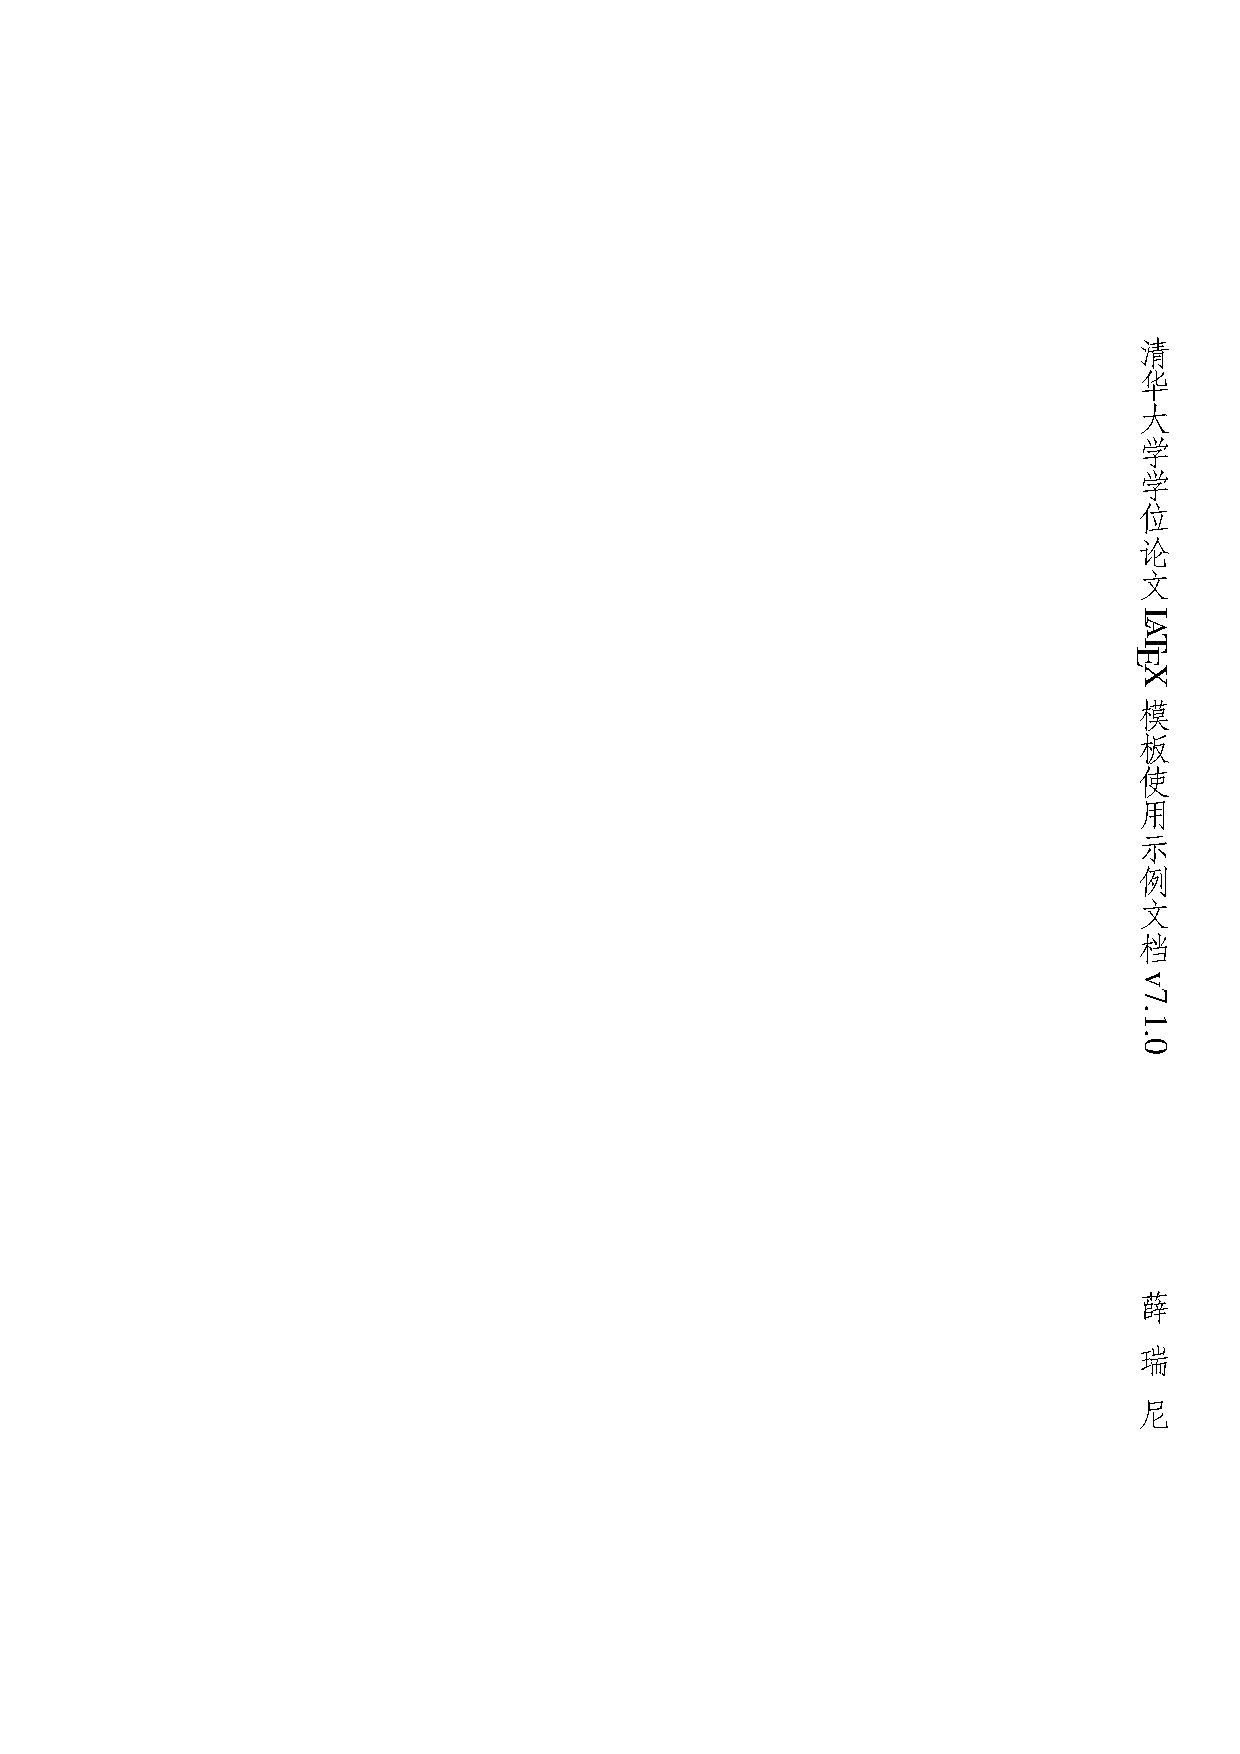
\includepdf[pages=1]{spine.pdf}%
}
\newcommand\thu@spine{%
  \ifthu@cjk@font@fandol
    \thu@input@spine
  \else
    \ifthu@cjk@font@noto
      \thu@input@spine
    \else
      \spine
    \fi
  \fi
}
%    \end{macrocode}
% \end{macro}
%
%
% \subsection{其它}
% \label{sec:other}
%
% 借用 \cls{ltxdoc} 和 \cls{l3doc} 里面的几个命令方便写文档。
%    \begin{macrocode}
\DeclareRobustCommand\cs[1]{\texttt{\char`\\#1}}
\DeclareRobustCommand\file{\nolinkurl}
\DeclareRobustCommand\env{\textsf}
\DeclareRobustCommand\pkg{\textsf}
\DeclareRobustCommand\cls{\textsf}
%    \end{macrocode}
%
%    \begin{macrocode}
\sloppy
%</cls>
%    \end{macrocode}
%
%
% \iffalse
%    \begin{macrocode}
%<*dtx-style>
\ProvidesPackage{dtx-style}
\RequirePackage{hypdoc}
\RequirePackage{ifthen}
\RequirePackage{fontspec}[2017/01/20]
\RequirePackage{amsmath}
\RequirePackage{unicode-math}
\RequirePackage{siunitx}
\RequirePackage[UTF8,scheme=chinese]{ctex}
\RequirePackage[
  top=2.5cm, bottom=2.5cm,
  left=4cm, right=2cm,
  headsep=3mm]{geometry}
\RequirePackage{hologo}
\RequirePackage{array,longtable,booktabs}
\RequirePackage{listings}
\RequirePackage{fancyhdr}
\RequirePackage{xcolor}
\RequirePackage{enumitem}
\RequirePackage{etoolbox}
\RequirePackage{metalogo}

% Pretending the `amssymb` has been loaded.
% This should be removed after `markdown` v2.13.0.
\expandafter\def\csname ver@amssymb.sty\endcsname{0000/00/00}
\RequirePackage[tightLists=false]{markdown}
\expandafter\let\csname ver@amssymb.sty\endcsname\relax

\markdownSetup{
  renderers = {
    link = {\href{#2}{#1}},
  }
}

\hypersetup{
  pdflang     = zh-CN,
  pdftitle    = {SUSTechThesis:南方科技大学学位论文模板},
  pdfauthor   = {南方科技大学计算机研究协会 CRA},
  pdfsubject  = {南方科技大学学位论文模板使用说明},
  pdfkeywords = {论文模板; 南方科技大学; 使用说明},
  pdfdisplaydoctitle = true
}%

\ifthenelse{\equal{\@nameuse{g__ctex_fontset_tl}}{mac}}{
  \setmainfont{Palatino}
  \setsansfont[Scale=MatchLowercase]{Helvetica}
  \setmonofont[Scale=MatchLowercase]{Menlo}
  \xeCJKsetwidth{‘’“”}{1em}
}{
  \setmainfont[
    Extension      = .otf,
    UprightFont    = *-regular,
    BoldFont       = *-bold,
    ItalicFont     = *-italic,
    BoldItalicFont = *-bolditalic,
  ]{texgyrepagella}
  \setsansfont[
    Extension      = .otf,
    UprightFont    = *-regular,
    BoldFont       = *-bold,
    ItalicFont     = *-italic,
    BoldItalicFont = *-bolditalic,
  ]{texgyreheros}
  \setmonofont[
    Extension      = .otf,
    UprightFont    = *-regular,
    BoldFont       = *-bold,
    ItalicFont     = *-italic,
    BoldItalicFont = *-bolditalic,
    Scale          = MatchLowercase,
    Ligatures      = CommonOff,
  ]{texgyrecursor}
}
\unimathsetup{
  math-style=ISO,
  bold-style=ISO,
}
\IfFontExistsTF{XITSMath-Regular.otf}{
  \setmathfont[
    Extension    = .otf,
    BoldFont     = XITSMath-Bold,
    StylisticSet = 8,
  ]{XITSMath-Regular}
  \setmathfont[range={cal,bfcal},StylisticSet=1]{XITSMath-Regular.otf}
}{
  \setmathfont[
    Extension    = .otf,
    BoldFont     = *bold,
    StylisticSet = 8,
  ]{xits-math}
  \setmathfont[range={cal,bfcal},StylisticSet=1]{xits-math.otf}
}

\colorlet{thu@macro}{blue!60!black}
\colorlet{thu@env}{blue!70!black}
\colorlet{thu@option}{purple}
\patchcmd{\PrintMacroName}{\MacroFont}{\MacroFont\bfseries\color{thu@macro}}{}{}
\patchcmd{\PrintDescribeMacro}{\MacroFont}{\MacroFont\bfseries\color{thu@macro}}{}{}
\patchcmd{\PrintDescribeEnv}{\MacroFont}{\MacroFont\bfseries\color{thu@env}}{}{}
\patchcmd{\PrintEnvName}{\MacroFont}{\MacroFont\bfseries\color{thu@env}}{}{}

\def\DescribeOption{%
  \leavevmode\@bsphack\begingroup\MakePrivateLetters%
  \Describe@Option}
\def\Describe@Option#1{\endgroup
  \marginpar{\raggedleft\PrintDescribeOption{#1}}%
  \thu@special@index{option}{#1}\@esphack\ignorespaces}
\def\PrintDescribeOption#1{\strut \MacroFont\bfseries\sffamily\color{thu@option} #1\ }
\def\thu@special@index#1#2{\@bsphack
  \begingroup
    \HD@target
    \let\HDorg@encapchar\encapchar
    \edef\encapchar usage{%
      \HDorg@encapchar hdclindex{\the\c@HD@hypercount}{usage}%
    }%
    \index{#2\actualchar{\string\ttfamily\space#2}
           (#1)\encapchar usage}%
    \index{#1:\levelchar#2\actualchar
           {\string\ttfamily\space#2}\encapchar usage}%
  \endgroup
  \@esphack}

\lstdefinestyle{lstStyleBase}{%
   basicstyle=\small\ttfamily,
   aboveskip=\medskipamount,
   belowskip=\medskipamount,
   lineskip=0pt,
   boxpos=c,
   showlines=false,
   extendedchars=true,
   upquote=true,
   tabsize=2,
   showtabs=false,
   showspaces=false,
   showstringspaces=false,
   numbers=none,
   linewidth=\linewidth,
   xleftmargin=4pt,
   xrightmargin=0pt,
   resetmargins=false,
   breaklines=true,
   breakatwhitespace=false,
   breakindent=0pt,
   breakautoindent=true,
   columns=flexible,
   keepspaces=true,
   gobble=4,
   framesep=3pt,
   rulesep=1pt,
   framerule=1pt,
   backgroundcolor=\color{gray!5},
   stringstyle=\color{green!40!black!100},
   keywordstyle=\bfseries\color{blue!50!black},
   commentstyle=\slshape\color{black!60}}

\lstdefinestyle{lstStyleShell}{%
   style=lstStyleBase,
   frame=l,
   rulecolor=\color{purple},
   language=bash}

\lstdefinestyle{lstStyleLaTeX}{%
   style=lstStyleBase,
   frame=l,
   rulecolor=\color{violet},
   language=[LaTeX]TeX}

\lstnewenvironment{latex}{\lstset{style=lstStyleLaTeX}}{}
\lstnewenvironment{shell}{\lstset{style=lstStyleShell}}{}

\setlist{nosep}

\DeclareDocumentCommand{\option}{m}{\textsf{#1}}
\DeclareDocumentCommand{\env}{m}{\texttt{#1}}
\DeclareDocumentCommand{\pkg}{s m}{%
  \textsf{#2}\IfBooleanF#1{\thu@special@index{package}{#2}}}
\DeclareDocumentCommand{\cls}{s m}{%
  \textsf{#2}\IfBooleanF#1{\thu@special@index{package}{#2}}}
\DeclareDocumentCommand{\file}{s m}{%
  \nolinkurl{#2}\IfBooleanF#1{\thu@special@index{file}{#2}}}
\newcommand{\myentry}[1]{%
  \marginpar{\raggedleft\color{purple}\bfseries\strut #1}}
\newcommand{\note}[2][Note]{{%
  \color{magenta}{\bfseries #1}\emph{#2}}}

\DeclareDocumentCommand{\githubuser}{m}{\href{https://github.com/#1}{@#1}}

\def\thuthesis{\textsc{Thu}\-\textsc{Thesis}}
\def\sustechthesis{\textsc{SUSTech}\-\textsc{Thesis}}
%</dtx-style>
%    \end{macrocode}
% \fi
%
% \Finale
%
\endinput
% \iffalse
%  Local Variables:
%  mode: doctex
%  TeX-master: t
%  End:
% \fi
